\chapter{Results and Discussion}
\label{results}
The simulation, set-up as defined in the previous chapter, was run on a regular PC with an Intel Core i5 (\nth{8} Generation) chipset, running on AC power.


\section{Runtimes}
The total runtime for the simulation period (1 month) was \unit[2187]{s} or \unit[36.45]{min}.
As seen in Figures \ref{fig:run_vs_p} and \ref{fig:runtimes}, the number of internal time steps and thus the local simulation runtimes increase with increasing precipitation intensities and vice versa, thus automatically increasing temporal resolution where necessary and avoiding excessive computations where it is not necessary.
\begin{figure}[H]
    \centering
    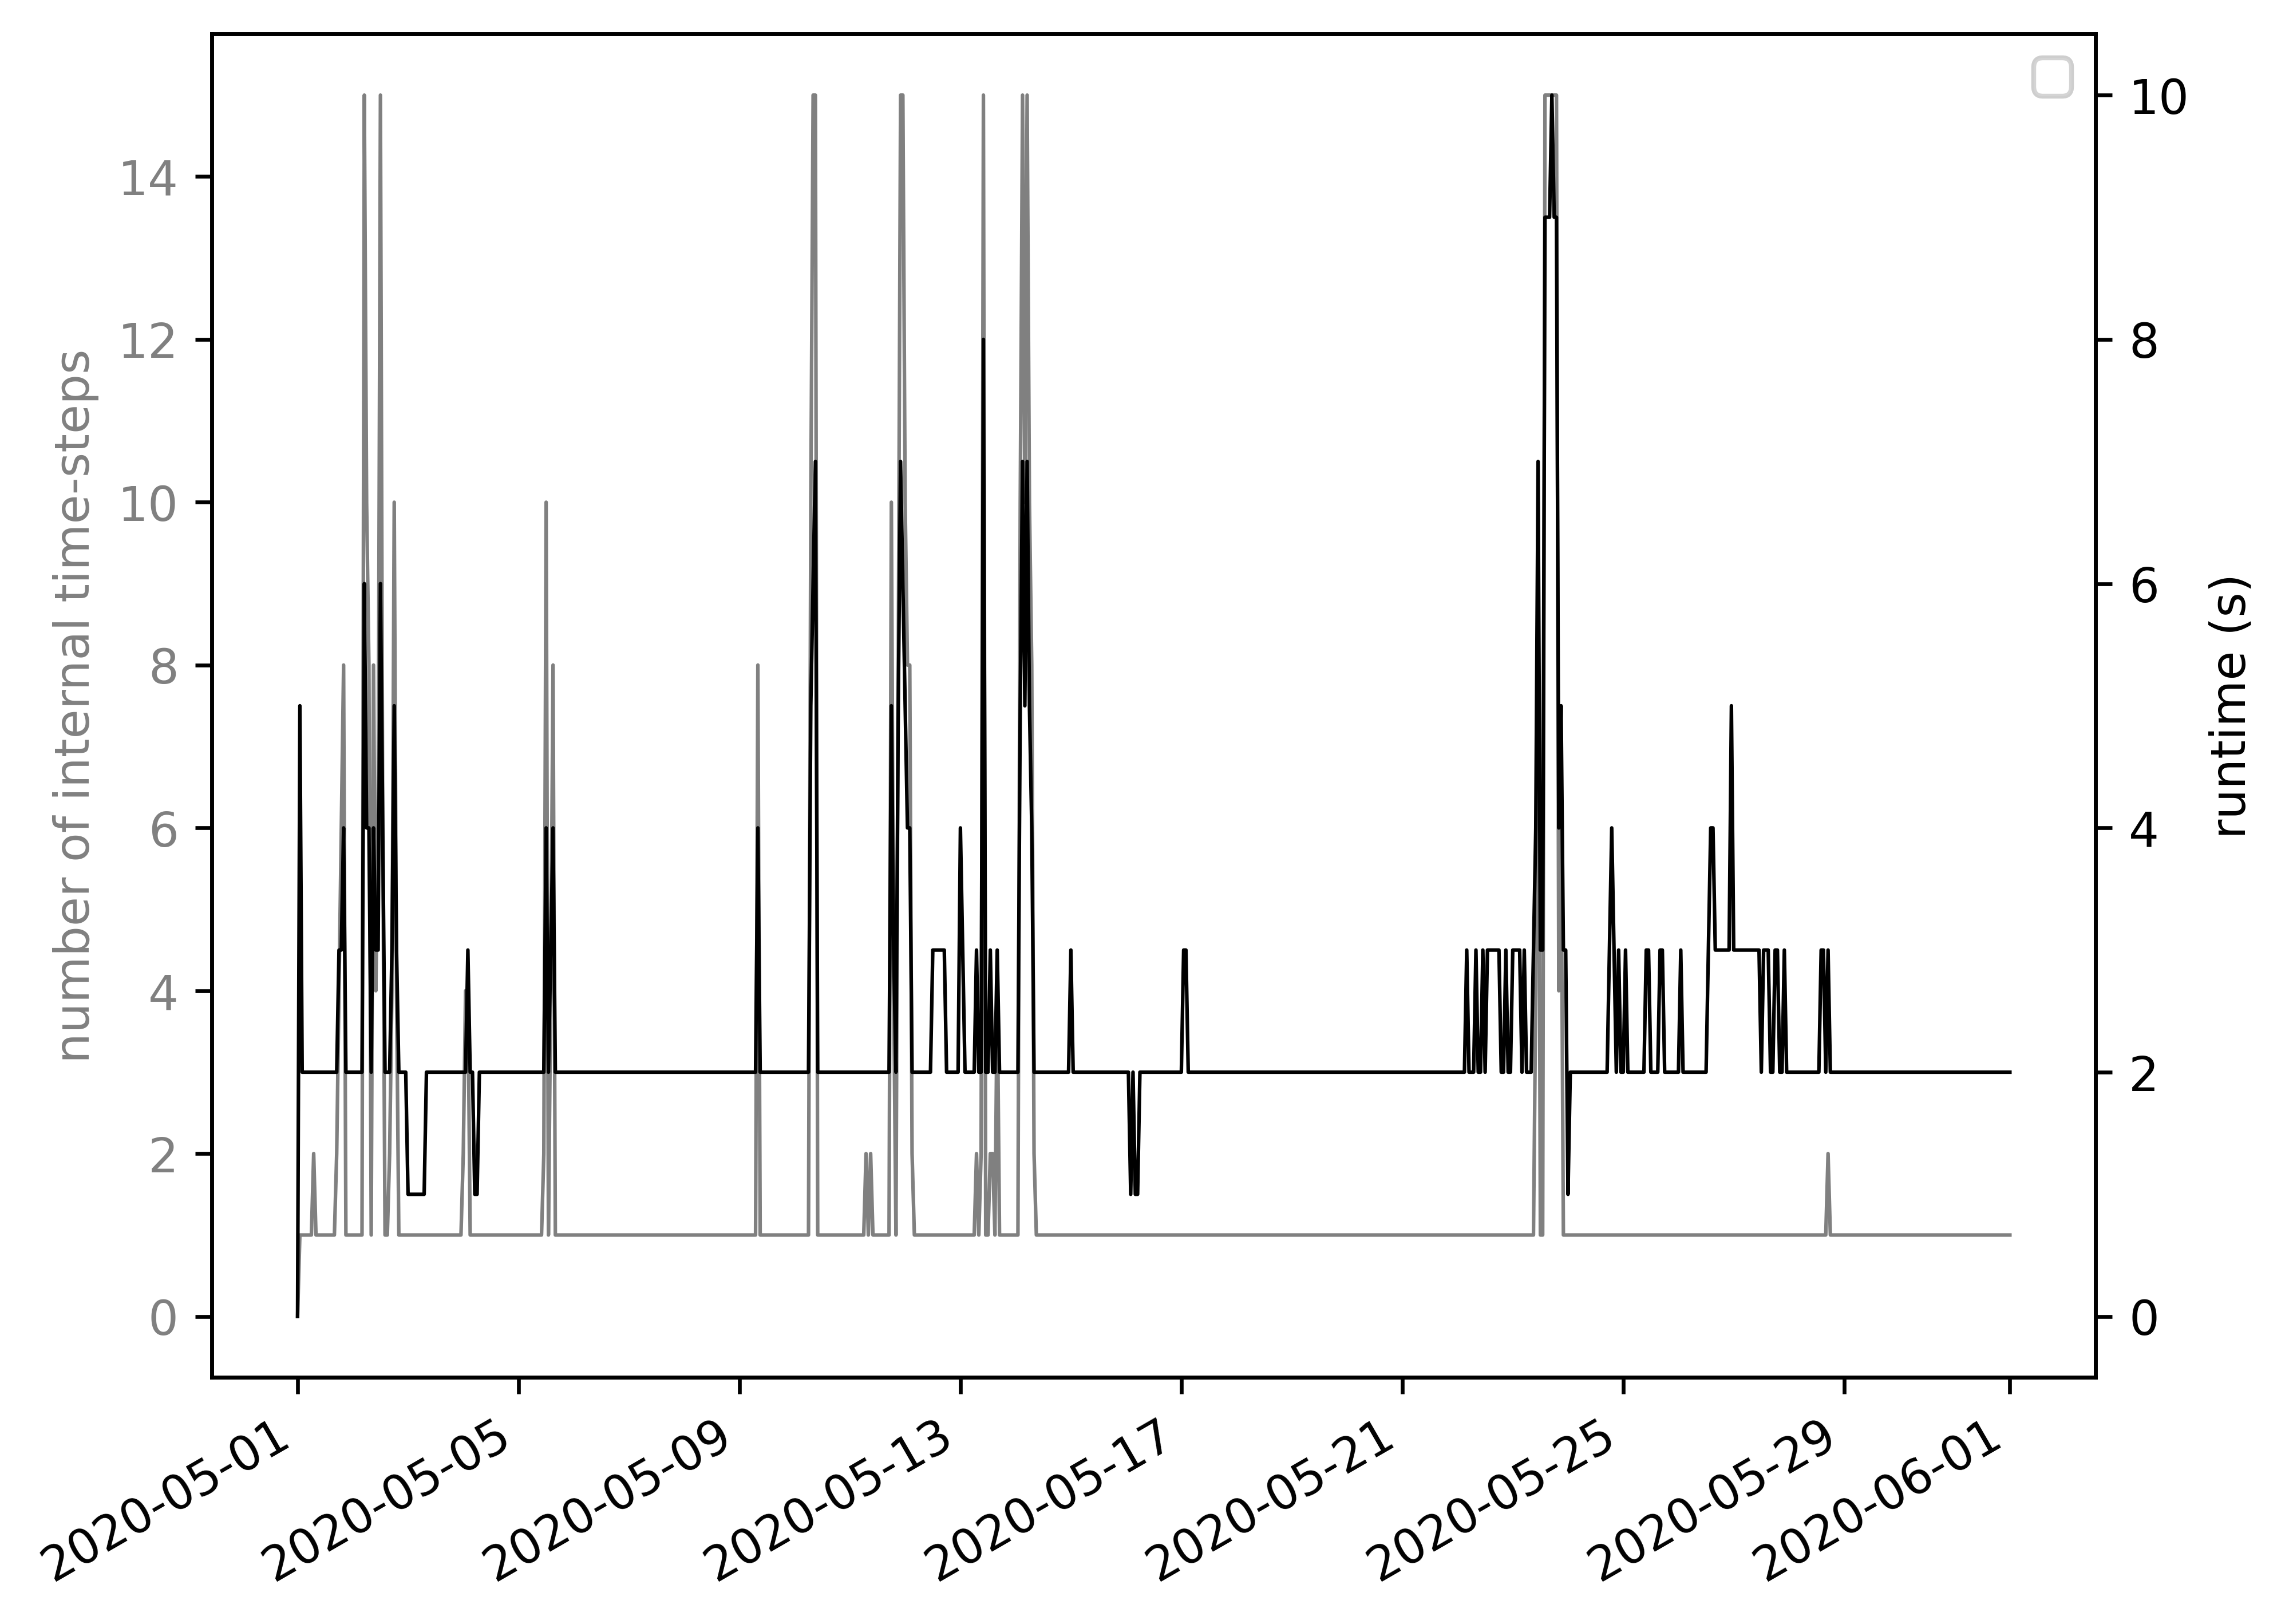
\includegraphics[width=\linewidth]{PICTURES/models_res/runtimes}
    \caption{Runtimes (s) and number of time-steps per local simulation period over the global simulation period.}
    \label{fig:runtimes}
\end{figure}
\begin{figure}[H]
    \centering
    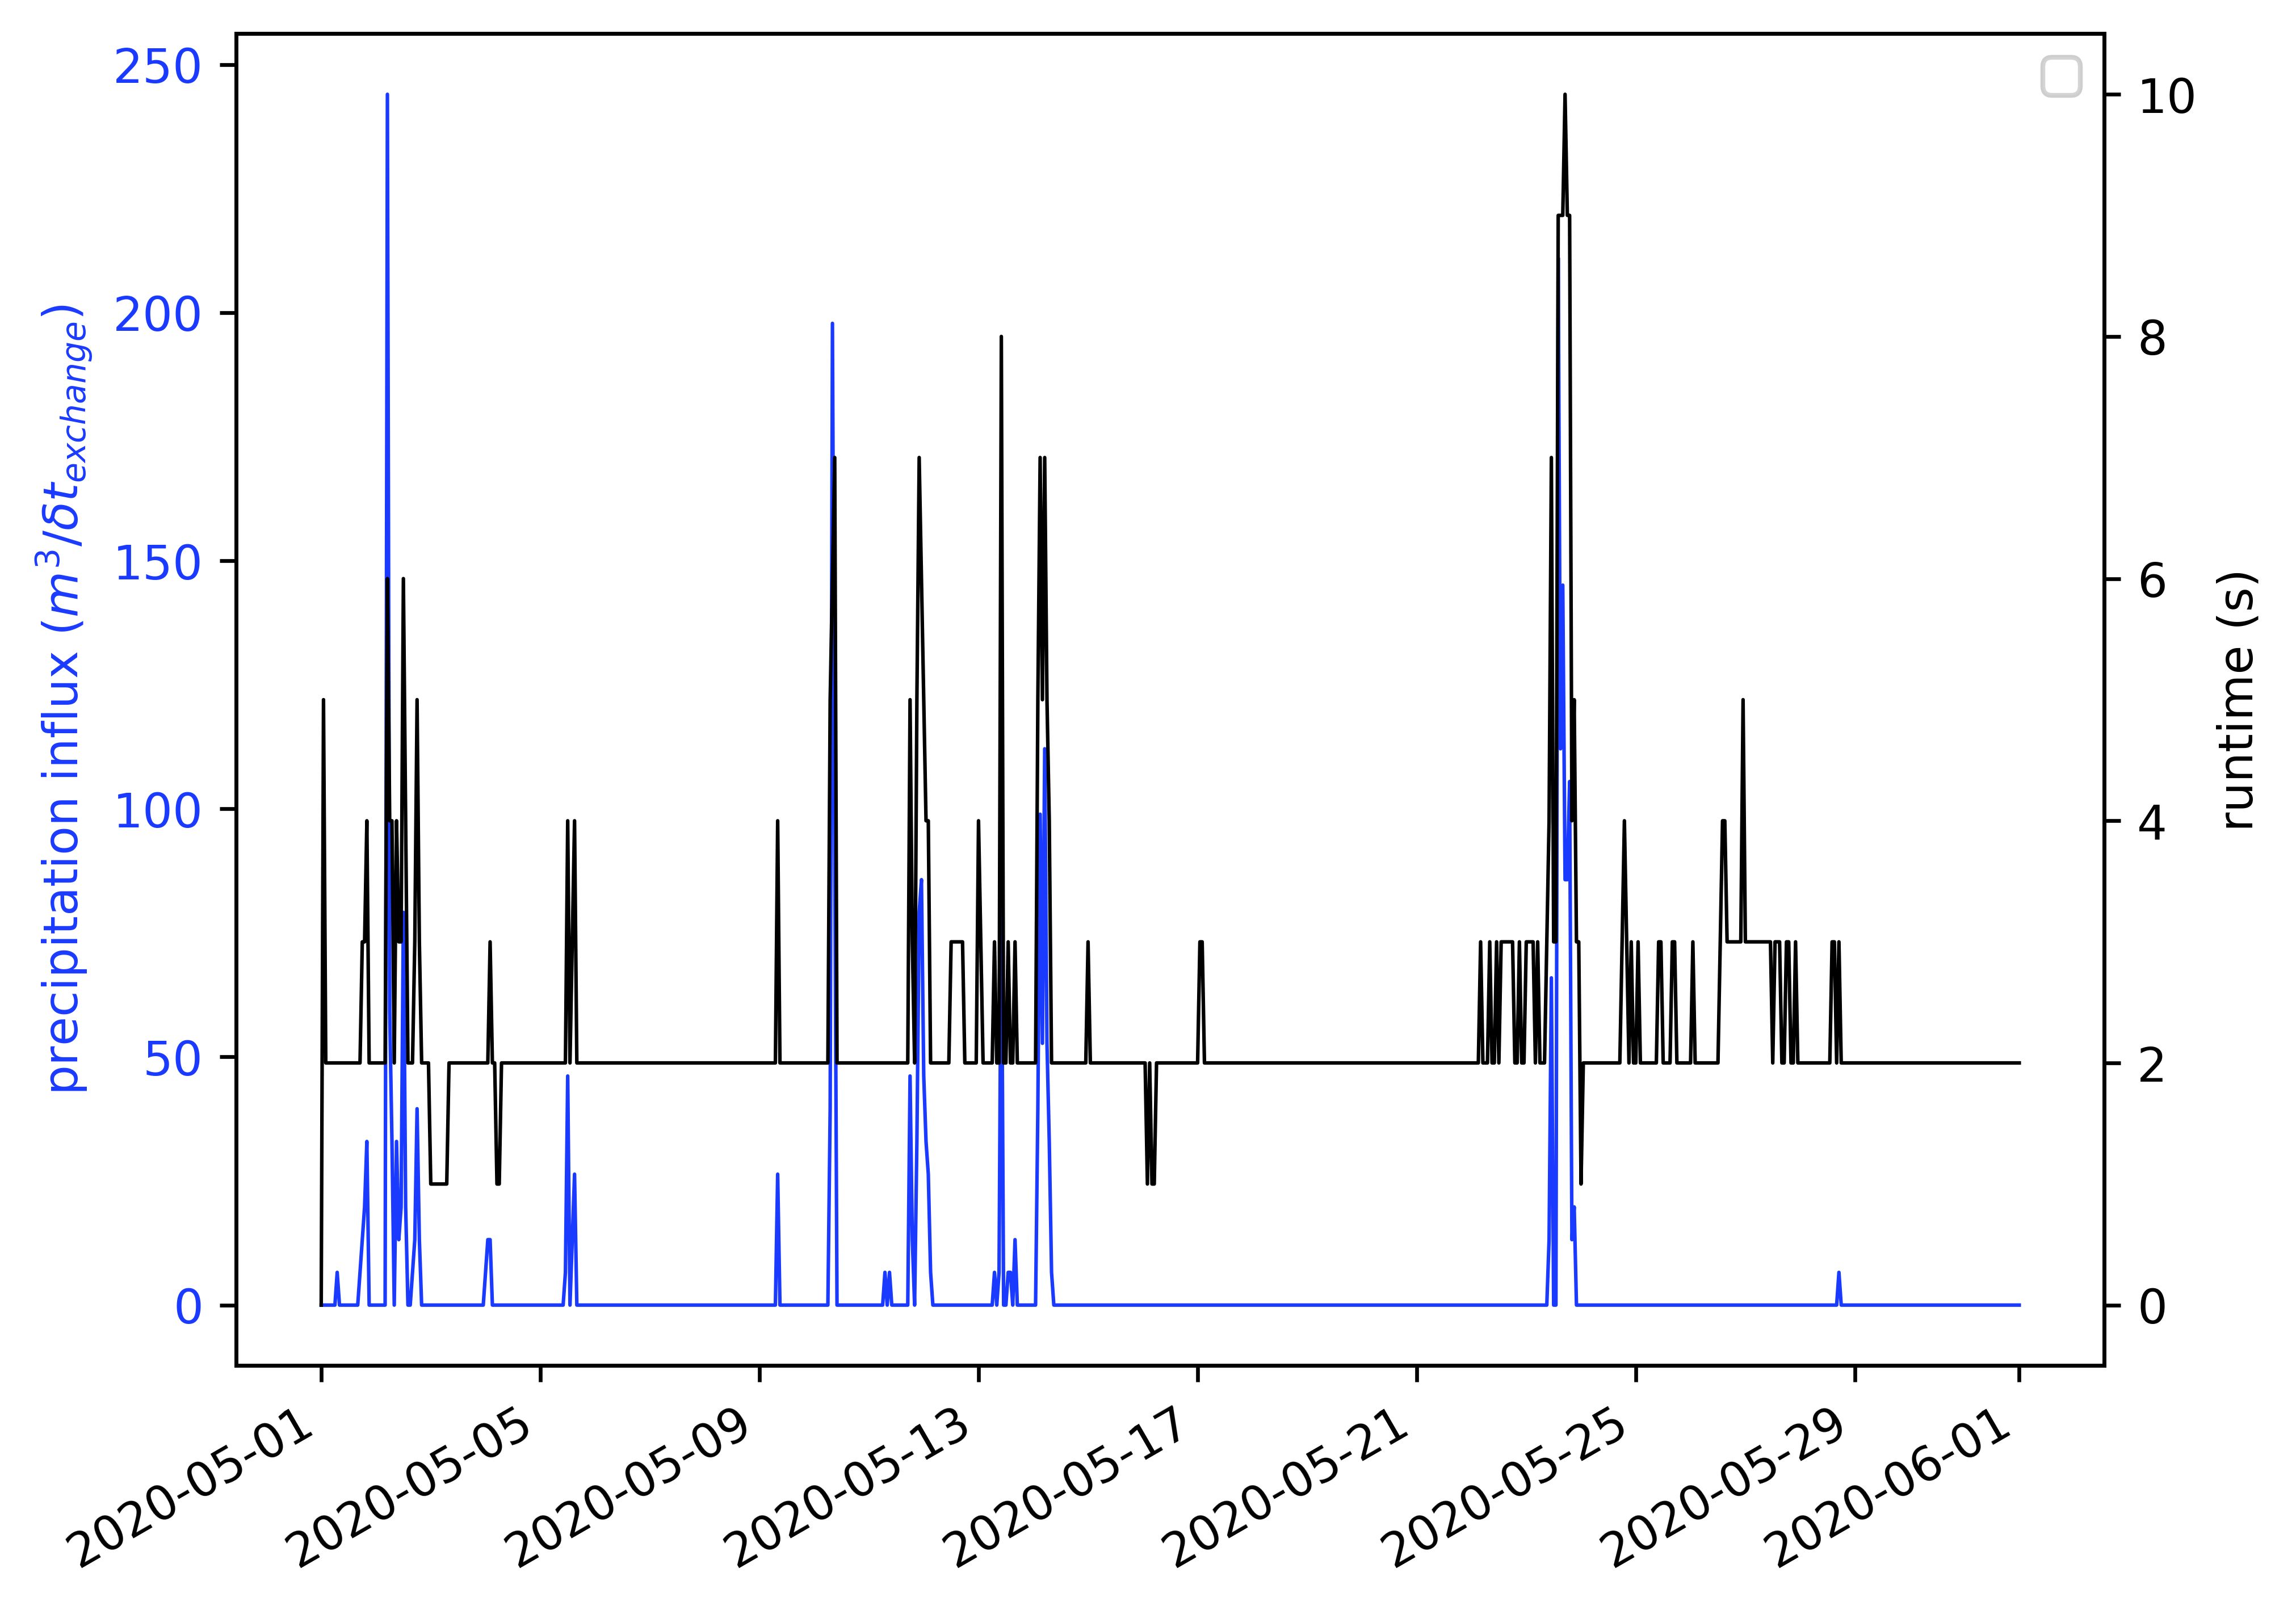
\includegraphics[width=\linewidth]{PICTURES/models_res/run_vs_p}
    \caption{Correlating precipitation intensities with Runtimes (s).}
    \label{fig:run_vs_p}
\end{figure}


\section{Mass Balance}
\label{mass_balance}
Figure \ref{fig:mass_balance_total} illustrates the mass balance of the GWSWEX model and the coupling scheme. It is safe to say that a good mass balance is achieved. The mass balance is calculated for each local simulation period as follows:
\begin{gather}
    \nonumber Q_{in} = P - ET \\
    \nonumber Q_{out} = SM_{dis} + GW_{dis} + SW_{dis}
\end{gather}

where
\begin{tabbing}
    $P$ \hspace{.4in}\= = precipitation influx in $m^3$,\\
    $ET$ \>= evapotranspiration outflux in $m^3$, \\ 
    $SM_{dis}$ \>= discharges in the SM storage term in $m^3$,\\
    $GW_{dis}$ \>= discharges in the GW storage term in $m^3$, and\\
    $SW_{dis}$ \>= discharges in the SW storage term in $m^3$.\\
\end{tabbing}


As seen in table \ref{tab:results} and the subsequent figures, the evapotranspiration outflux, owing to its volume, and precipitation influx follows it. \\

\begin{table}[H]
\caption{Consolidated summary of the simulation results}
\label{tab:results}
\centering
\begin{tabular}{lr}
\hline\noalign{\smallskip}
quantity & flux (in: +ve, out: -ve)  \\
\noalign{\smallskip}\hline\noalign{\smallskip}
evapotranspiration  & \SI{-5654.71}{\cubic\metre} \\
precipitation  & +\SI{2901.39}{\cubic\metre} \\
\hline\noalign{\smallskip}
IN, GWSWEX & \SI{-2753.32}{\cubic\metre} \\
\hline\noalign{\smallskip}
SM discharge & \SI{-3892.95}{\cubic\metre} \\
GW discharge & +\SI{1117.94}{\cubic\metre} \\
SW discharge & +\SI{7.51}{\cubic\metre} \\
\hline\noalign{\smallskip}
OUT, GWSWEX & \SI{-2767.52}{\cubic\metre} \\
\noalign{\smallskip}\hline
Error & \SI{-14.19}{\cubic\metre} (0.51\%) \\
\noalign{\smallskip}\hline
\end{tabular}
\end{table}

\subsection{Addressing the Discrepancy}
\begin{figure}[H]
    \centering
    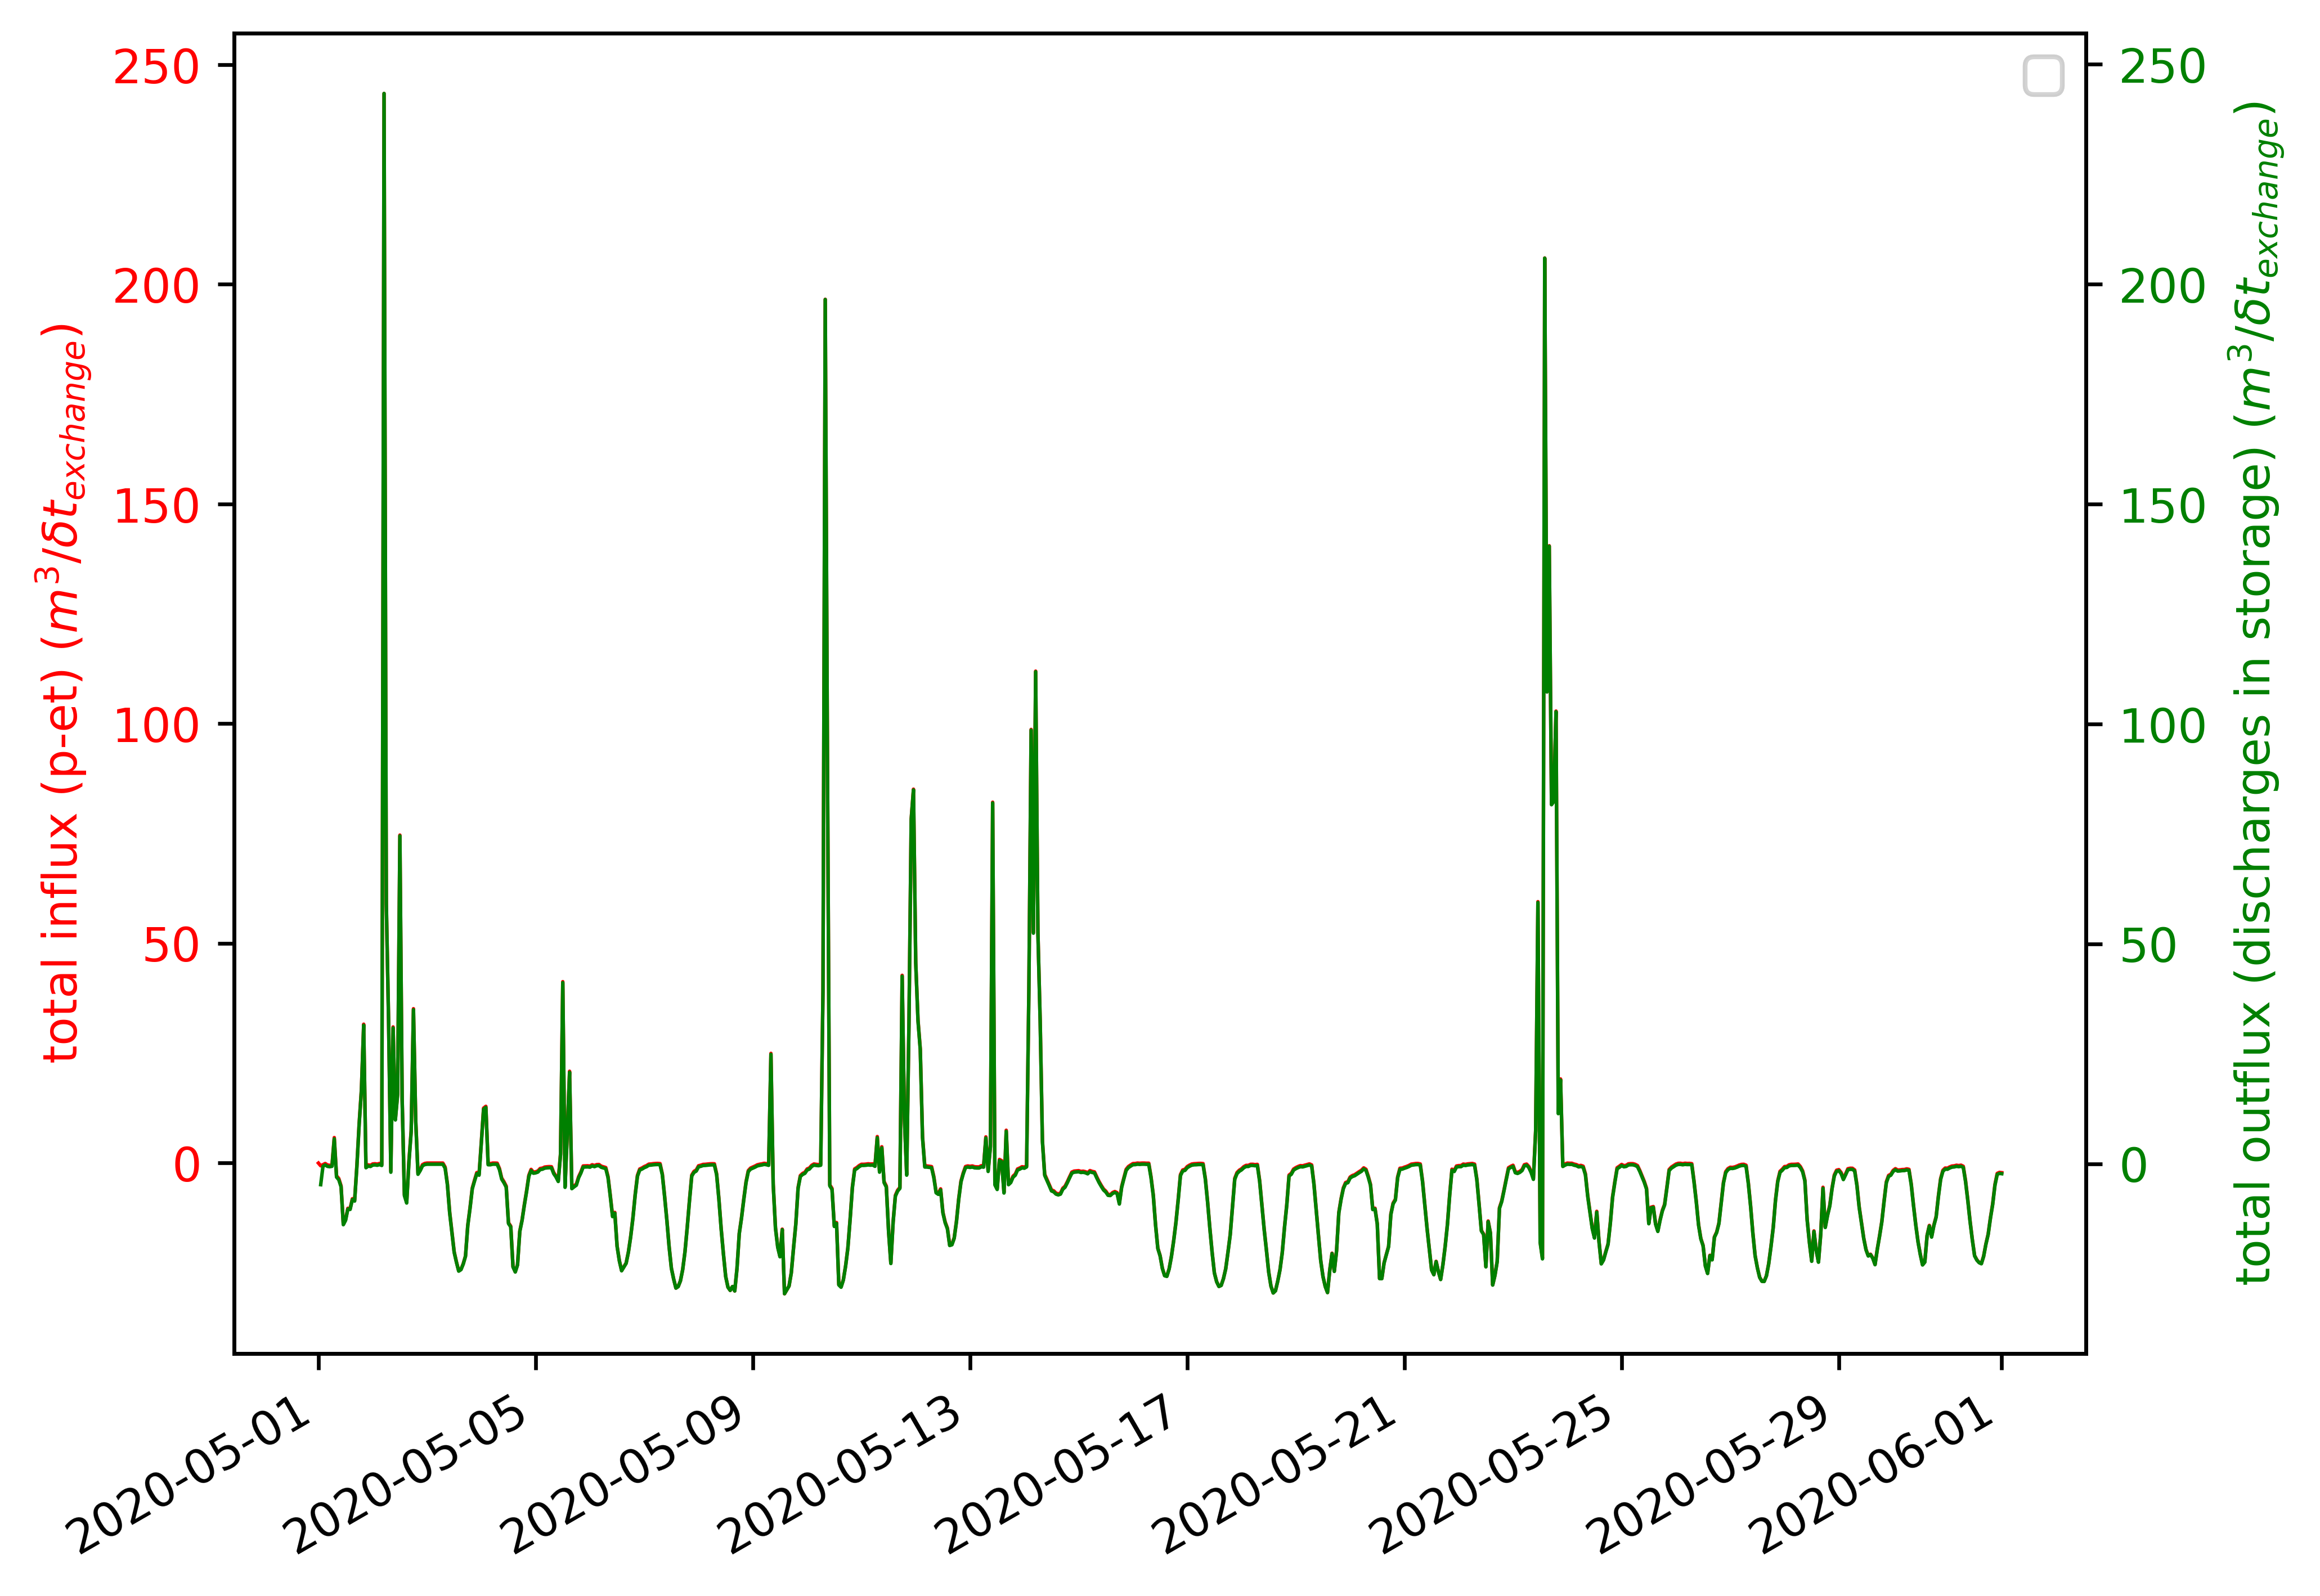
\includegraphics[width=\linewidth]{PICTURES/models_res/mass_balance}
    \caption{Mass balance.}
    \label{fig:mass_balance_total}
\end{figure}

The mass balance discrepancy can be attributed to a known flaw in the coupling scheme/SW model. It is documented that D-Flow FM relaxes negative lateral discharges with a factor of 0.5 when the storage is deemed \textit{inadequate}. However, it is not clearly defined what amount of storage is adequate to avoid relaxation of negative discharges. Figure \ref{fig:err_delft-fort} illustrates this discrepancy over the simulation period.
\begin{figure}[H]
    \centering
    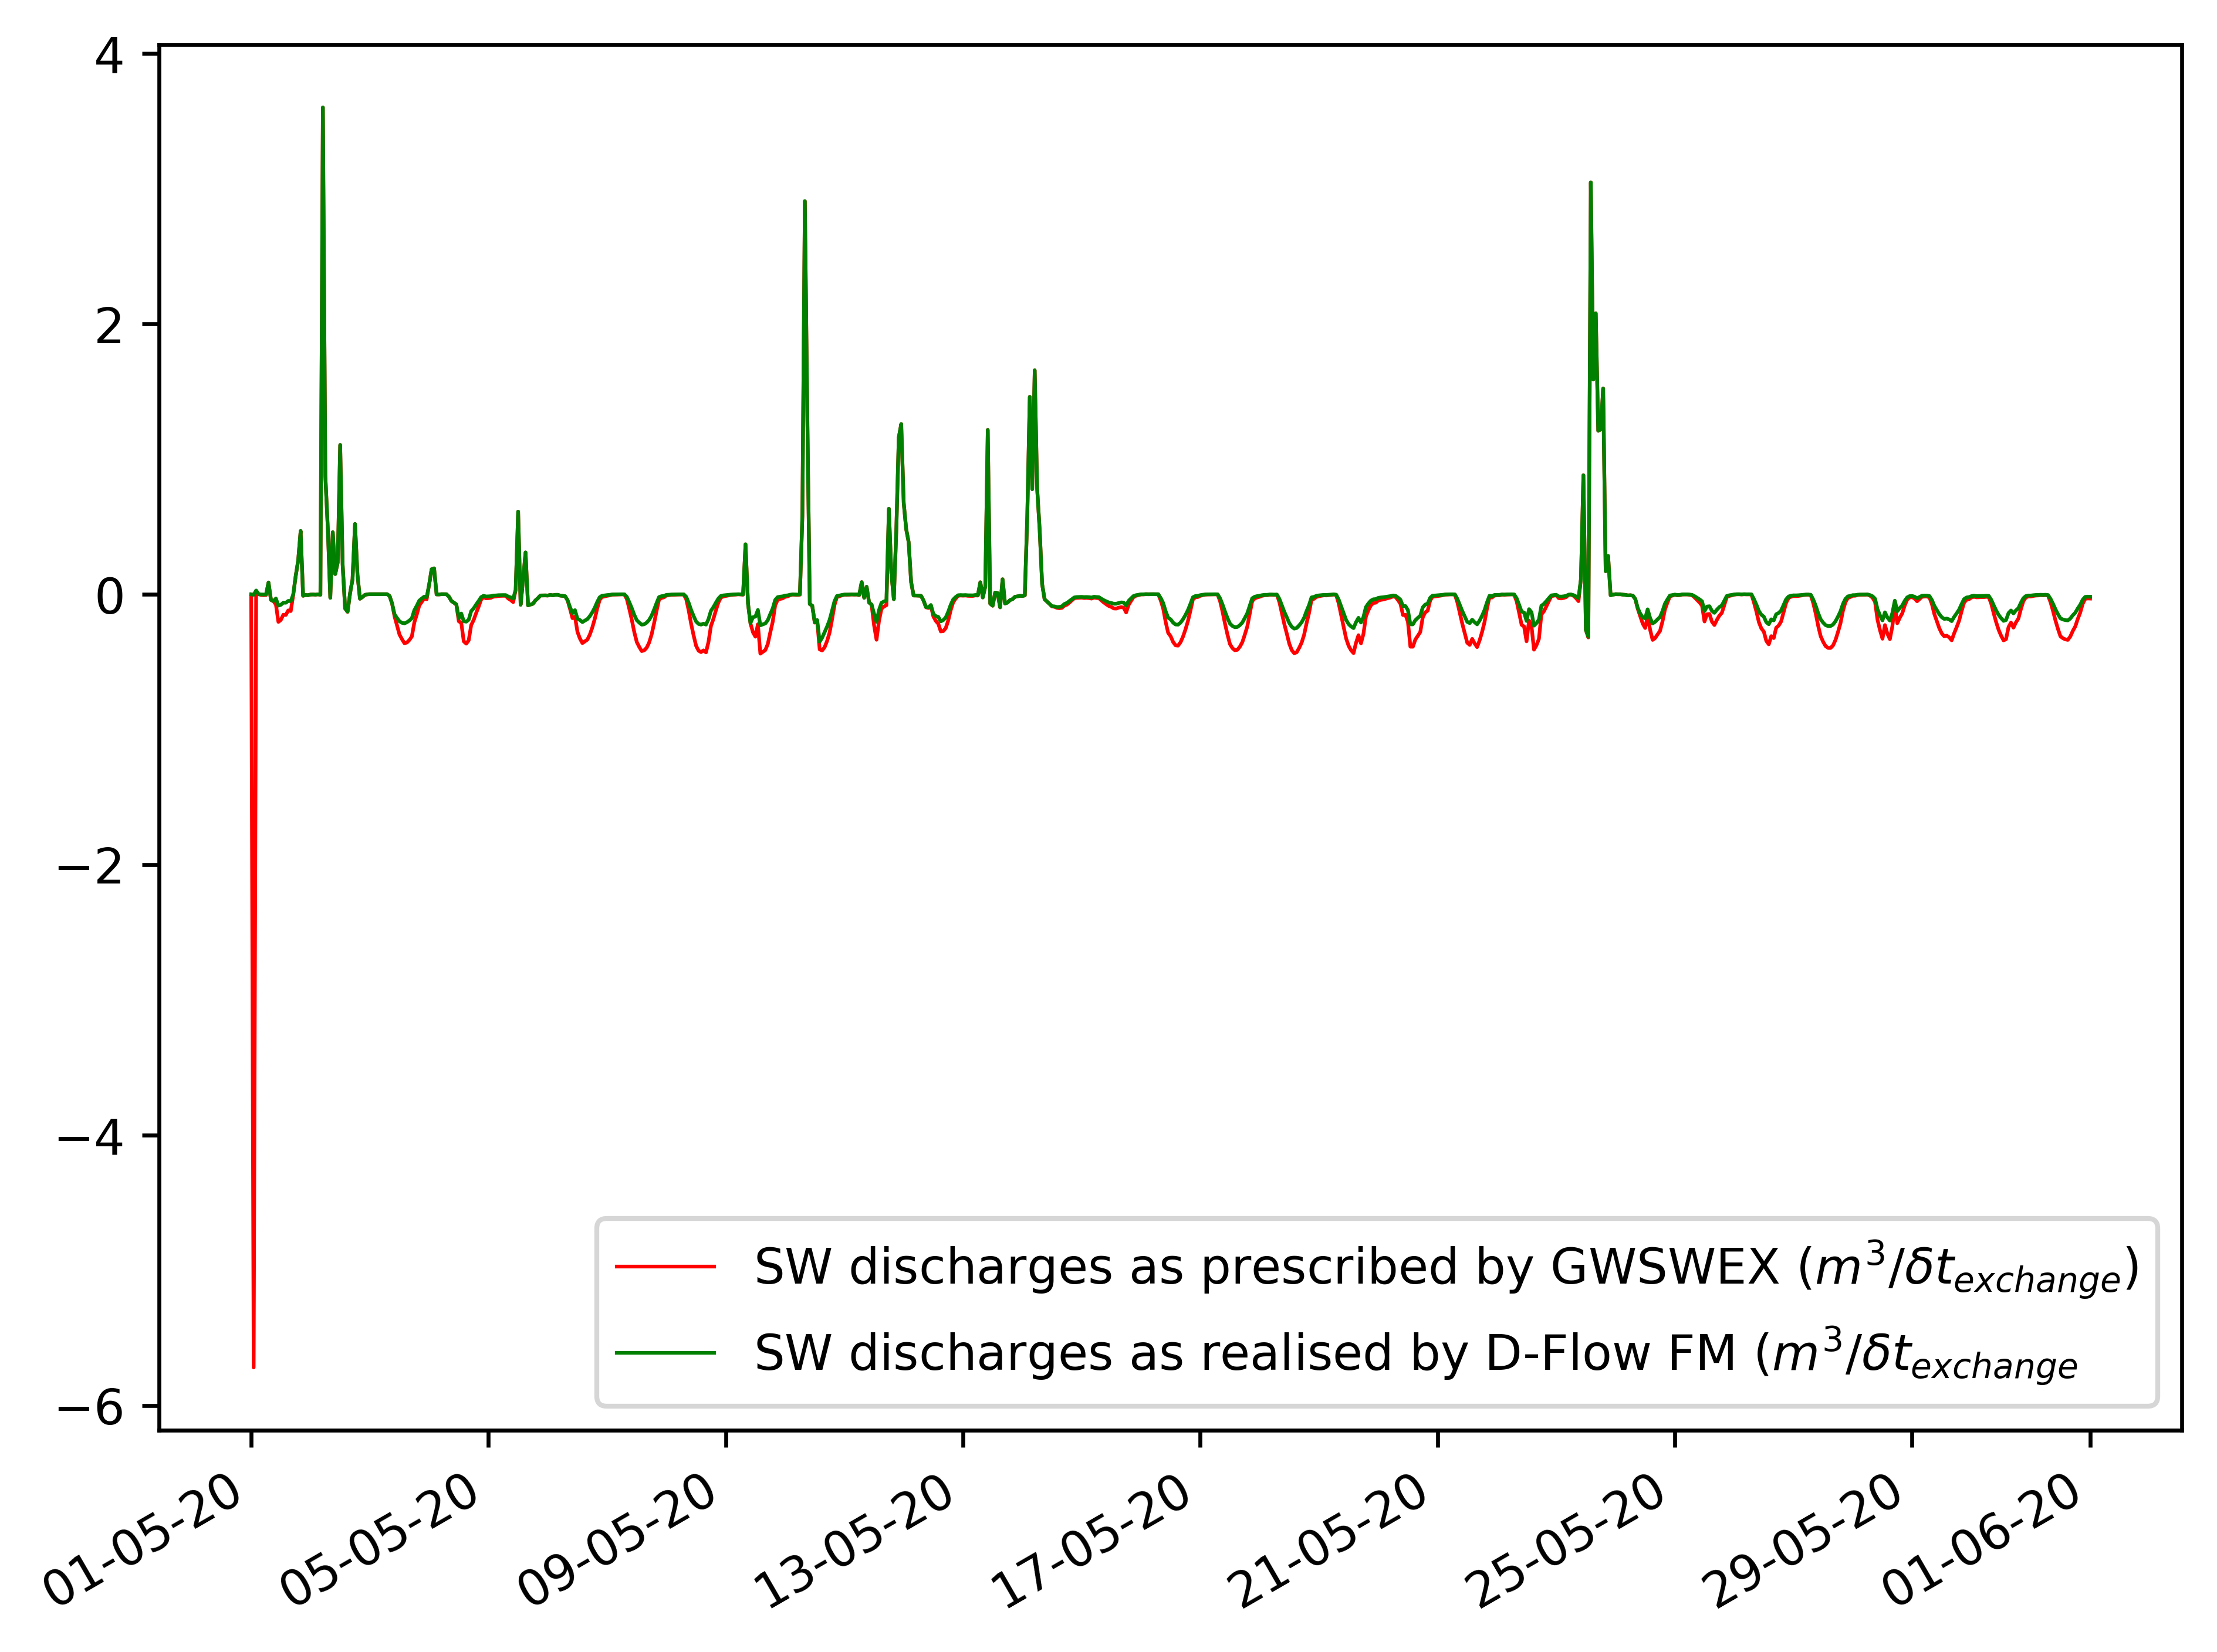
\includegraphics[width=\linewidth]{PICTURES/models_res/err_delft-fort}
    \caption{Discrepancy between prescribed and realised SW storage discharges.}
    \label{fig:err_delft-fort}
\end{figure}

The residual error in the GWSWEX model, as seen in Figure \ref{fig:err_fort} is rather negligible.
\begin{figure}[H]
    \centering
    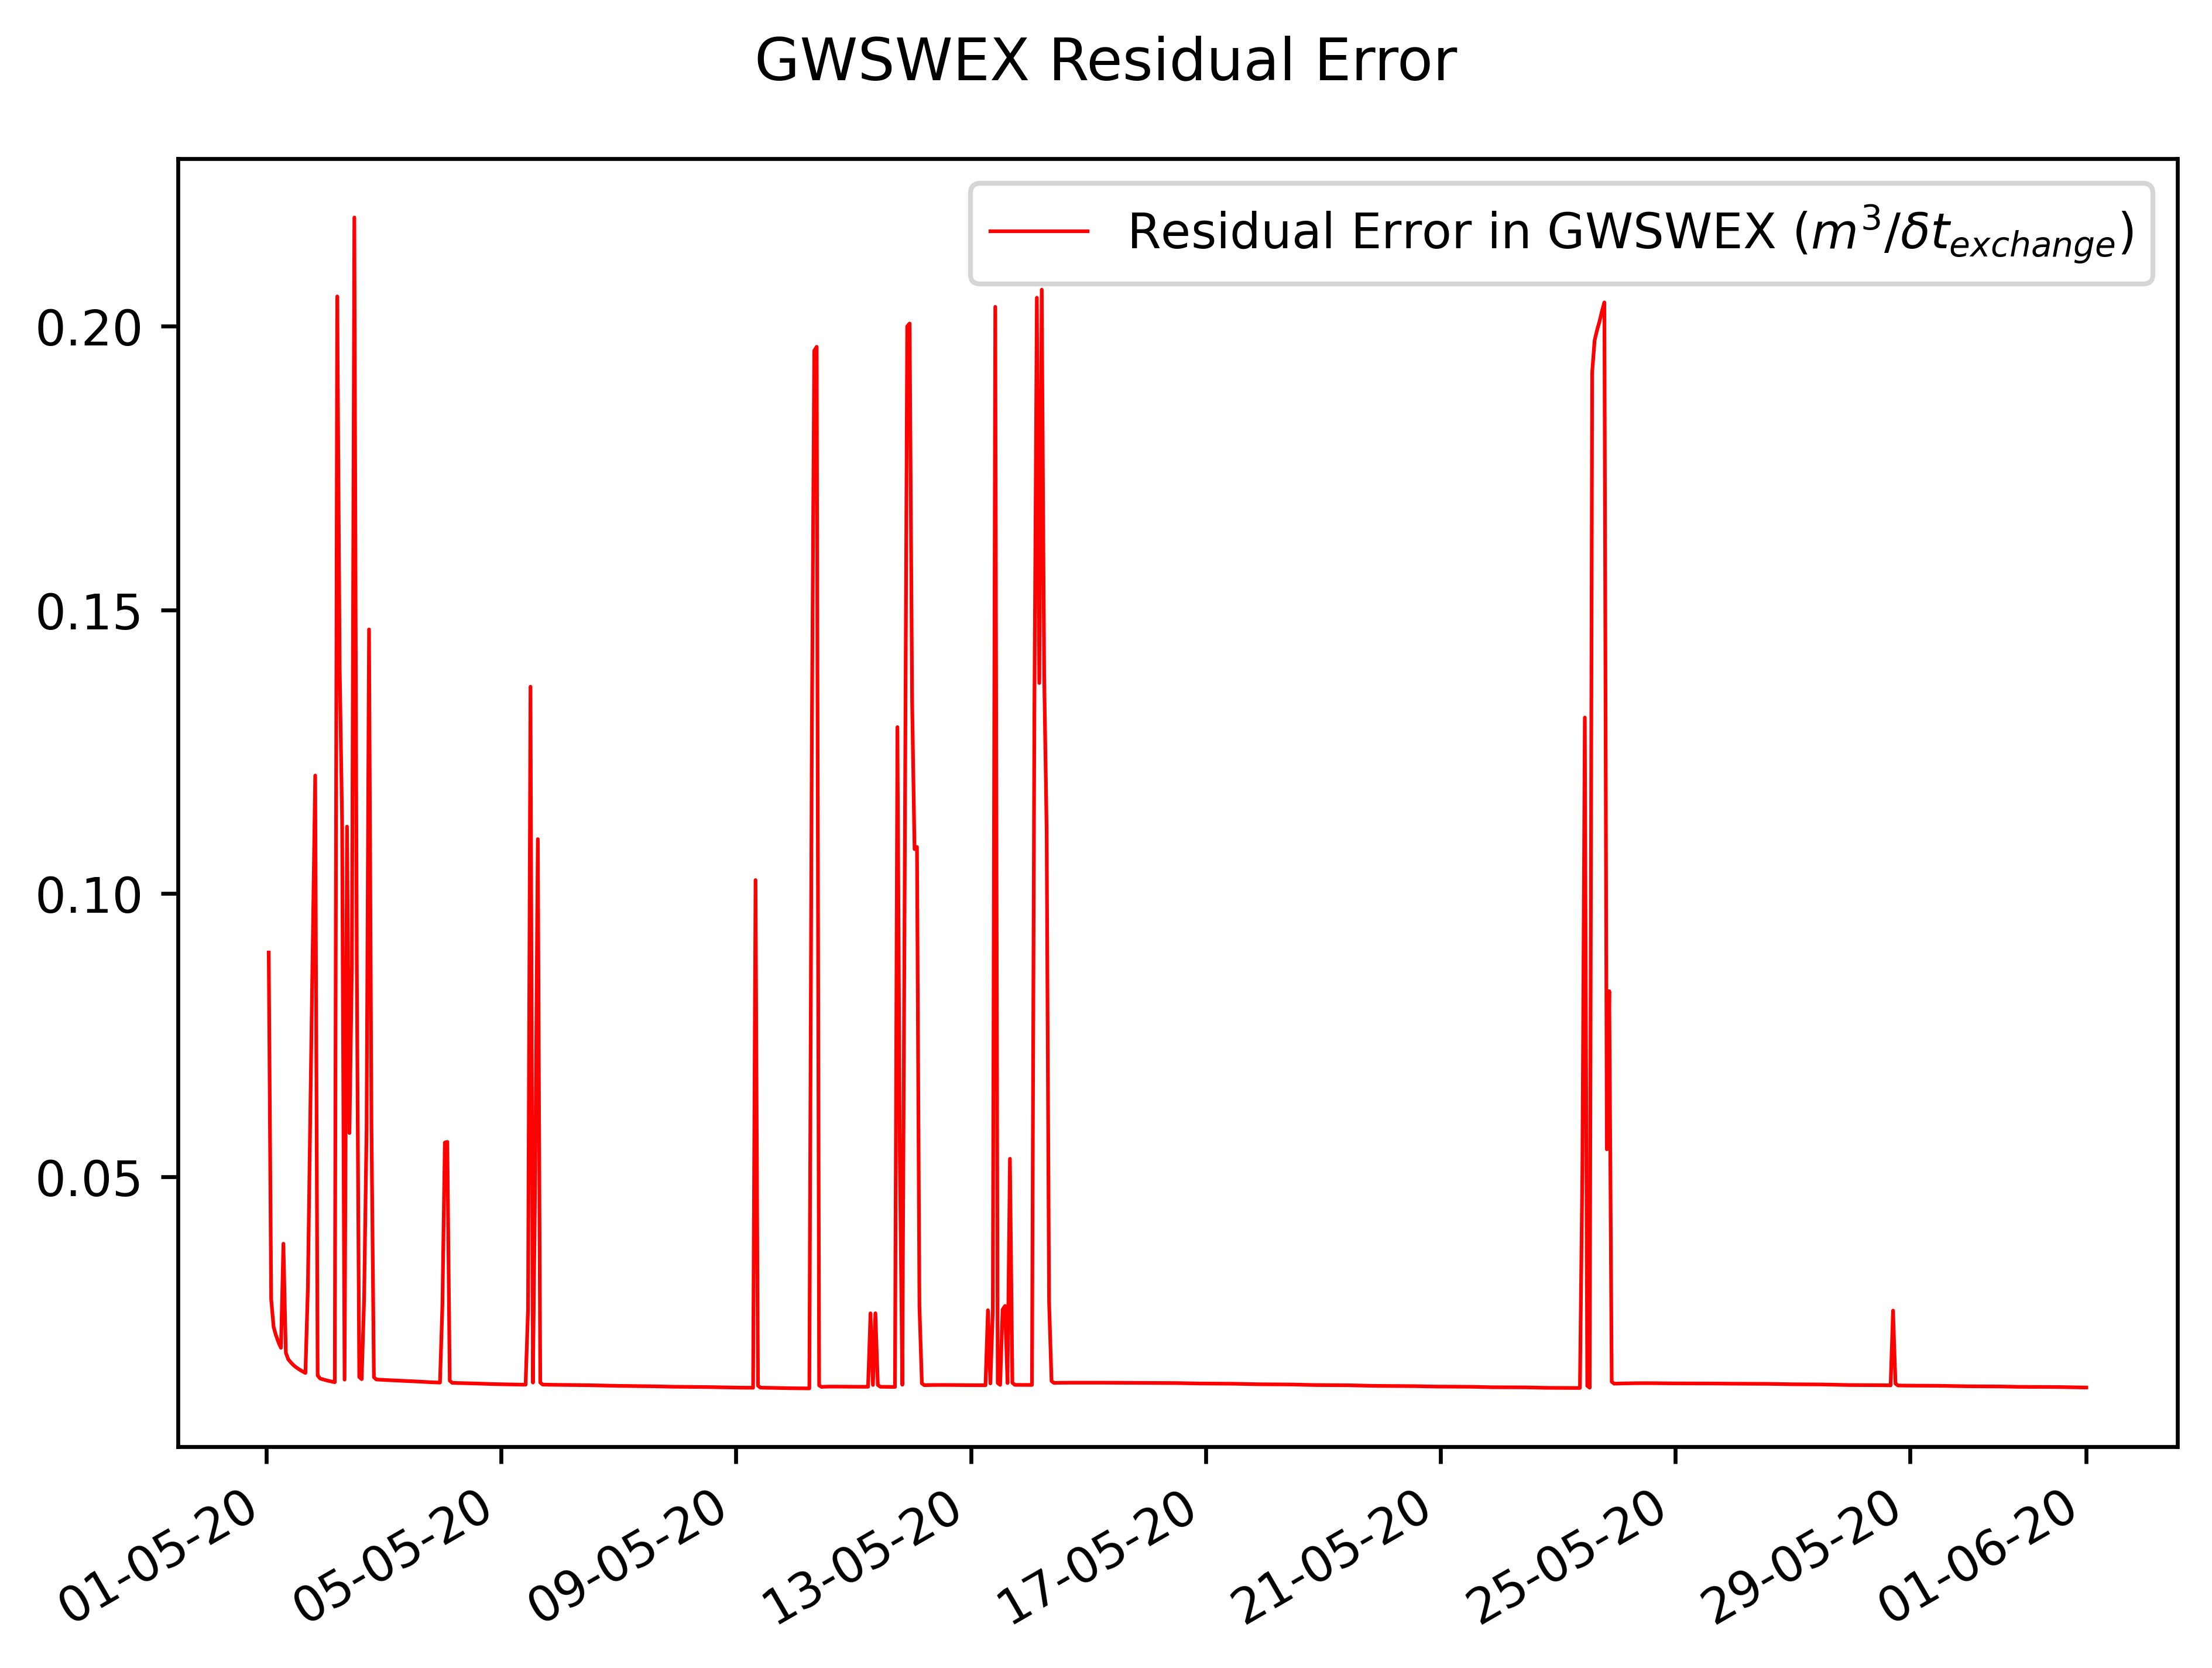
\includegraphics[width=\linewidth]{PICTURES/models_res/err_fort}
    \caption{Residual error in the GWSWEX model.}
    \label{fig:err_fort}
\end{figure}

\subsection{Following Evapotranspiration Outflux}
The following plots compare the ET outflux to the discharges in the three storages in an effort to both elucidate the behaviour of the model and to assess if the outcome is as one might expect.
\\ \\
As observed from Figures \ref{fig:et_vs_sm} and \ref{fig:et_vs_gw}, most of the ET outflux is satisfied by reduction in SM storage, especially until 26-05-2020, following which contribution from GW storage towards satisfying the ET outflux increases. This shift may have occurred as SM storage of a good portion of the model area, especially around the dewatering stream, has been reduced to $SM_\textrm{min}$ as seen in Figure \ref{fig:sm_res}. Increasing the GWSWEX model parameter, $m$, shall bring about this shift quicker and vice versa. One can observe, here, the consequence of this model parameter that defines the irreducible part of the SM storage - $SM_\textrm{min}$.
\\ \\
As was expected, contribution from the SW storage was negligible towards satisfying the ET outfluxes, as seen in Figure \ref{fig:et_vs_sw}.


\begin{figure}[H]
    \centering
    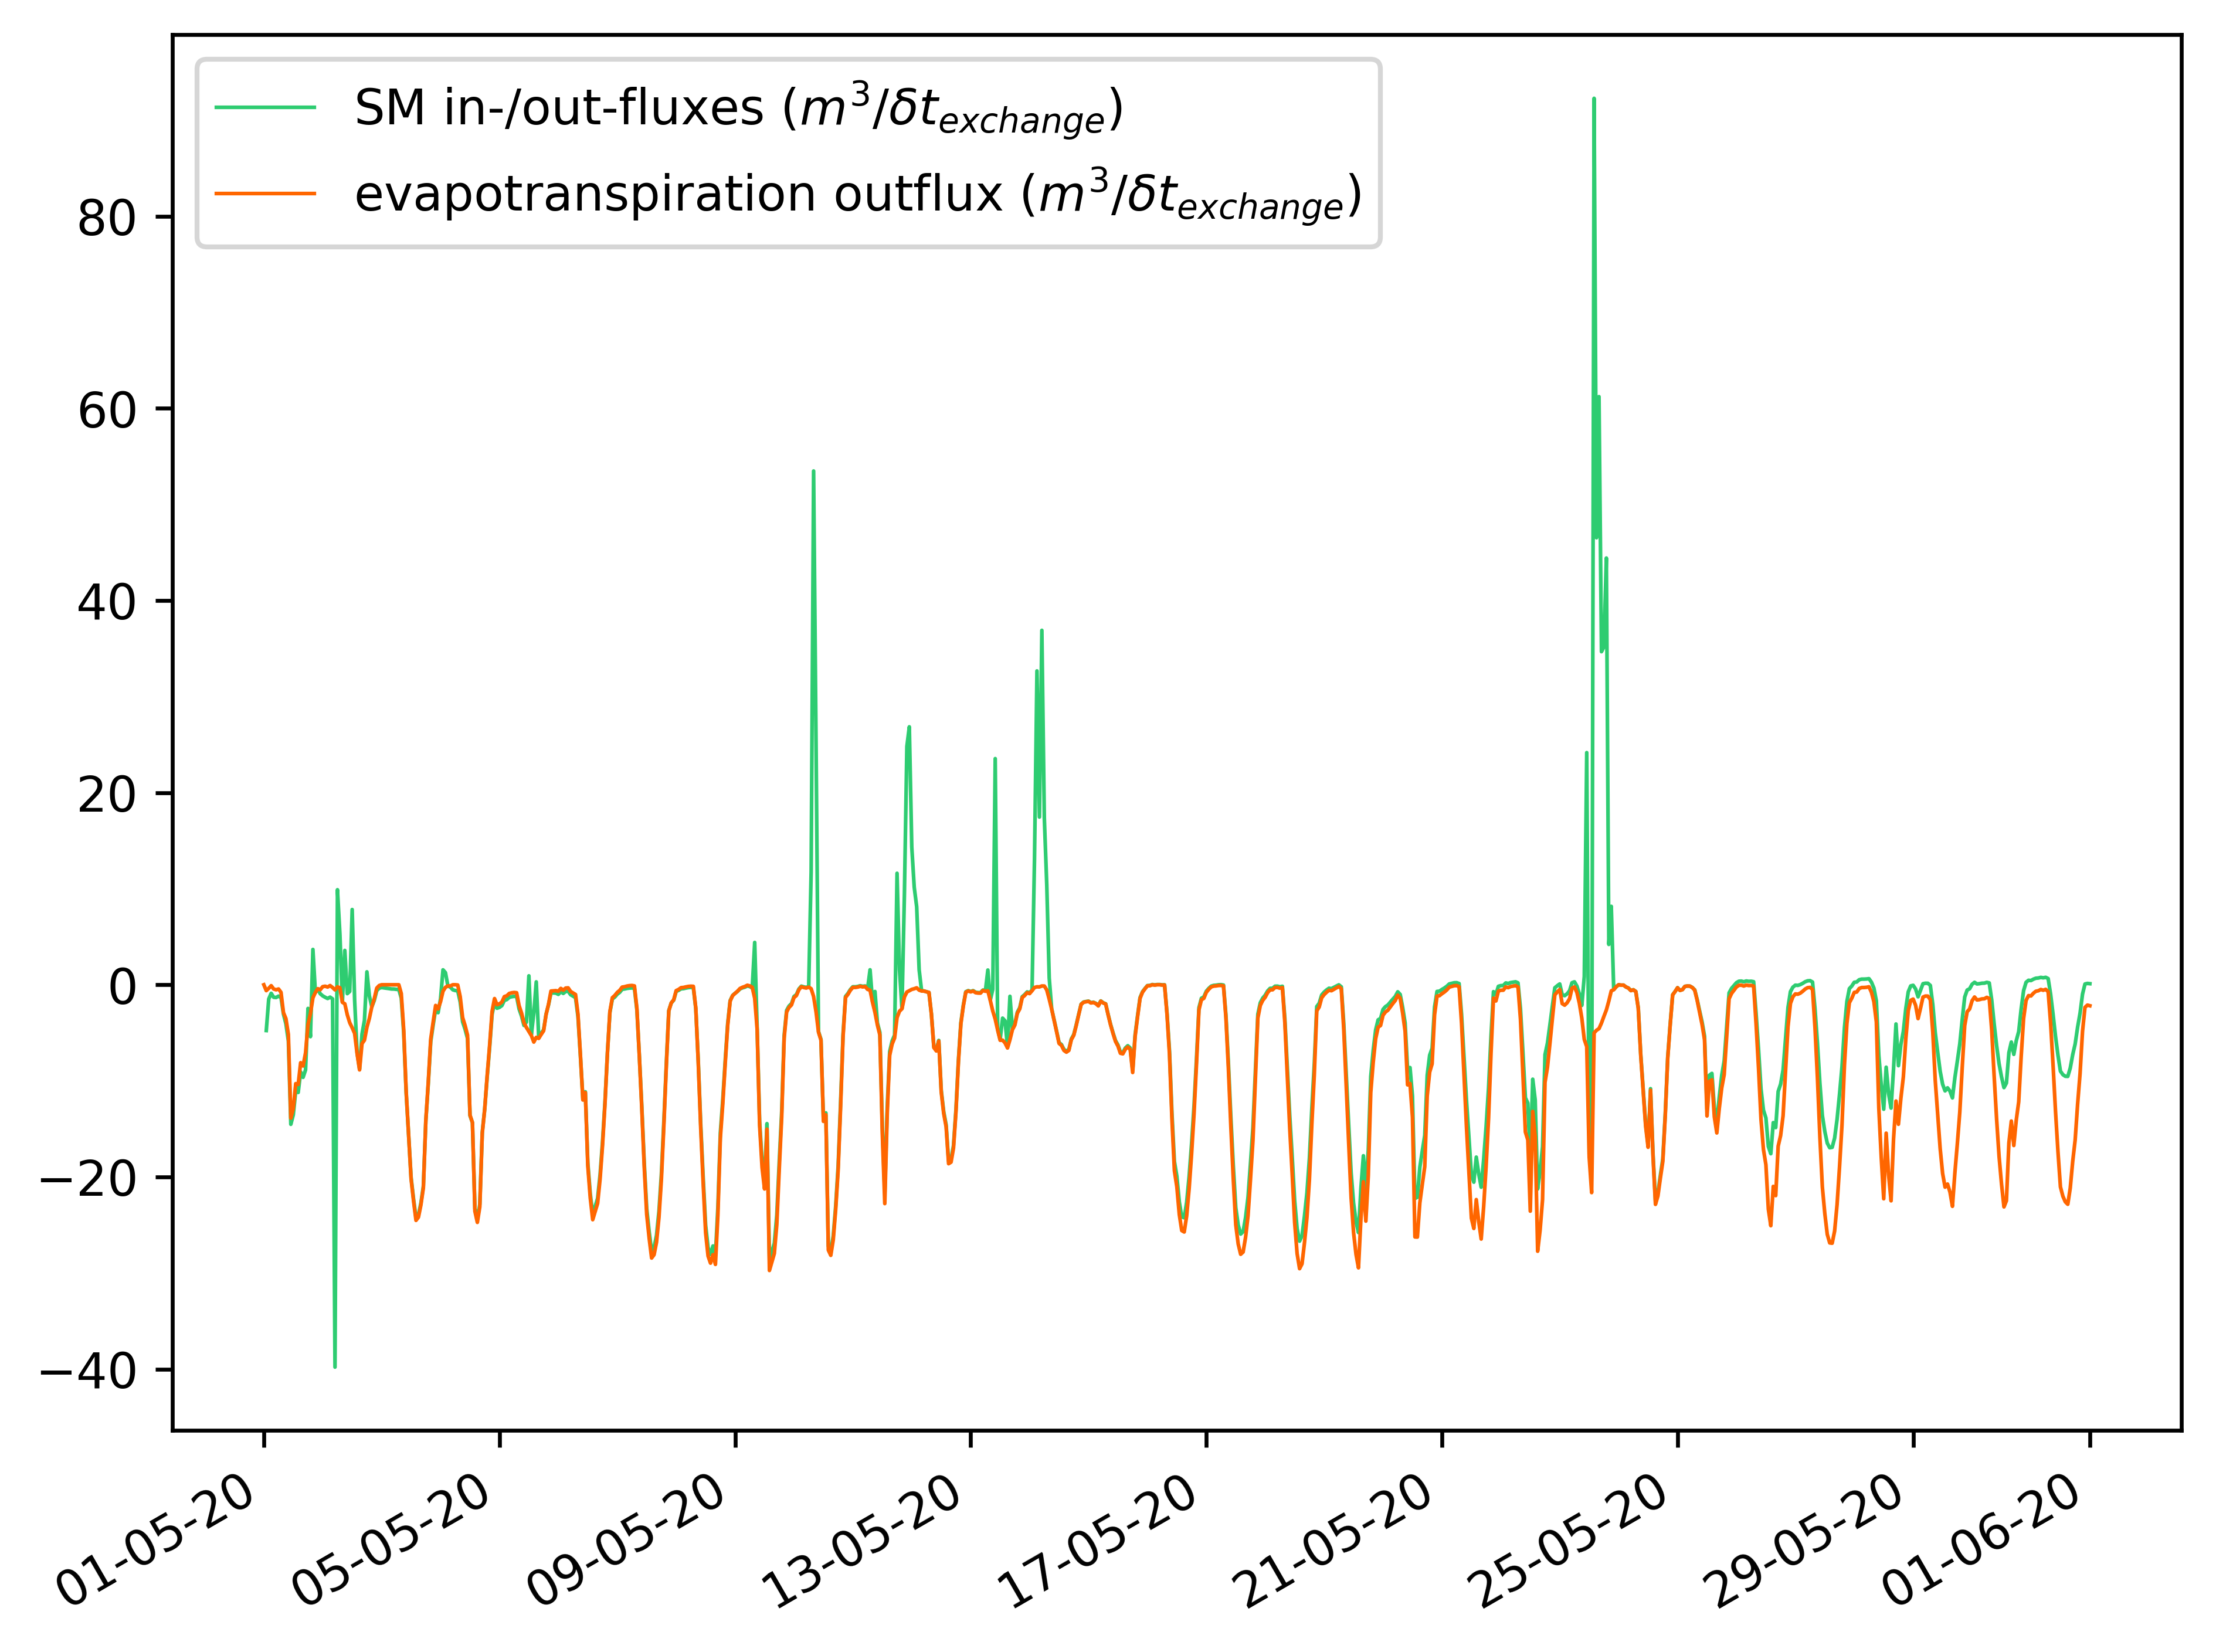
\includegraphics[height=0.42\textheight]{PICTURES/models_res/et_vs_sm}
    \caption{Comparing ET outfluxes with SM storage changes.}
    \label{fig:et_vs_sm}
\end{figure}
\begin{figure}[H]
    \centering
    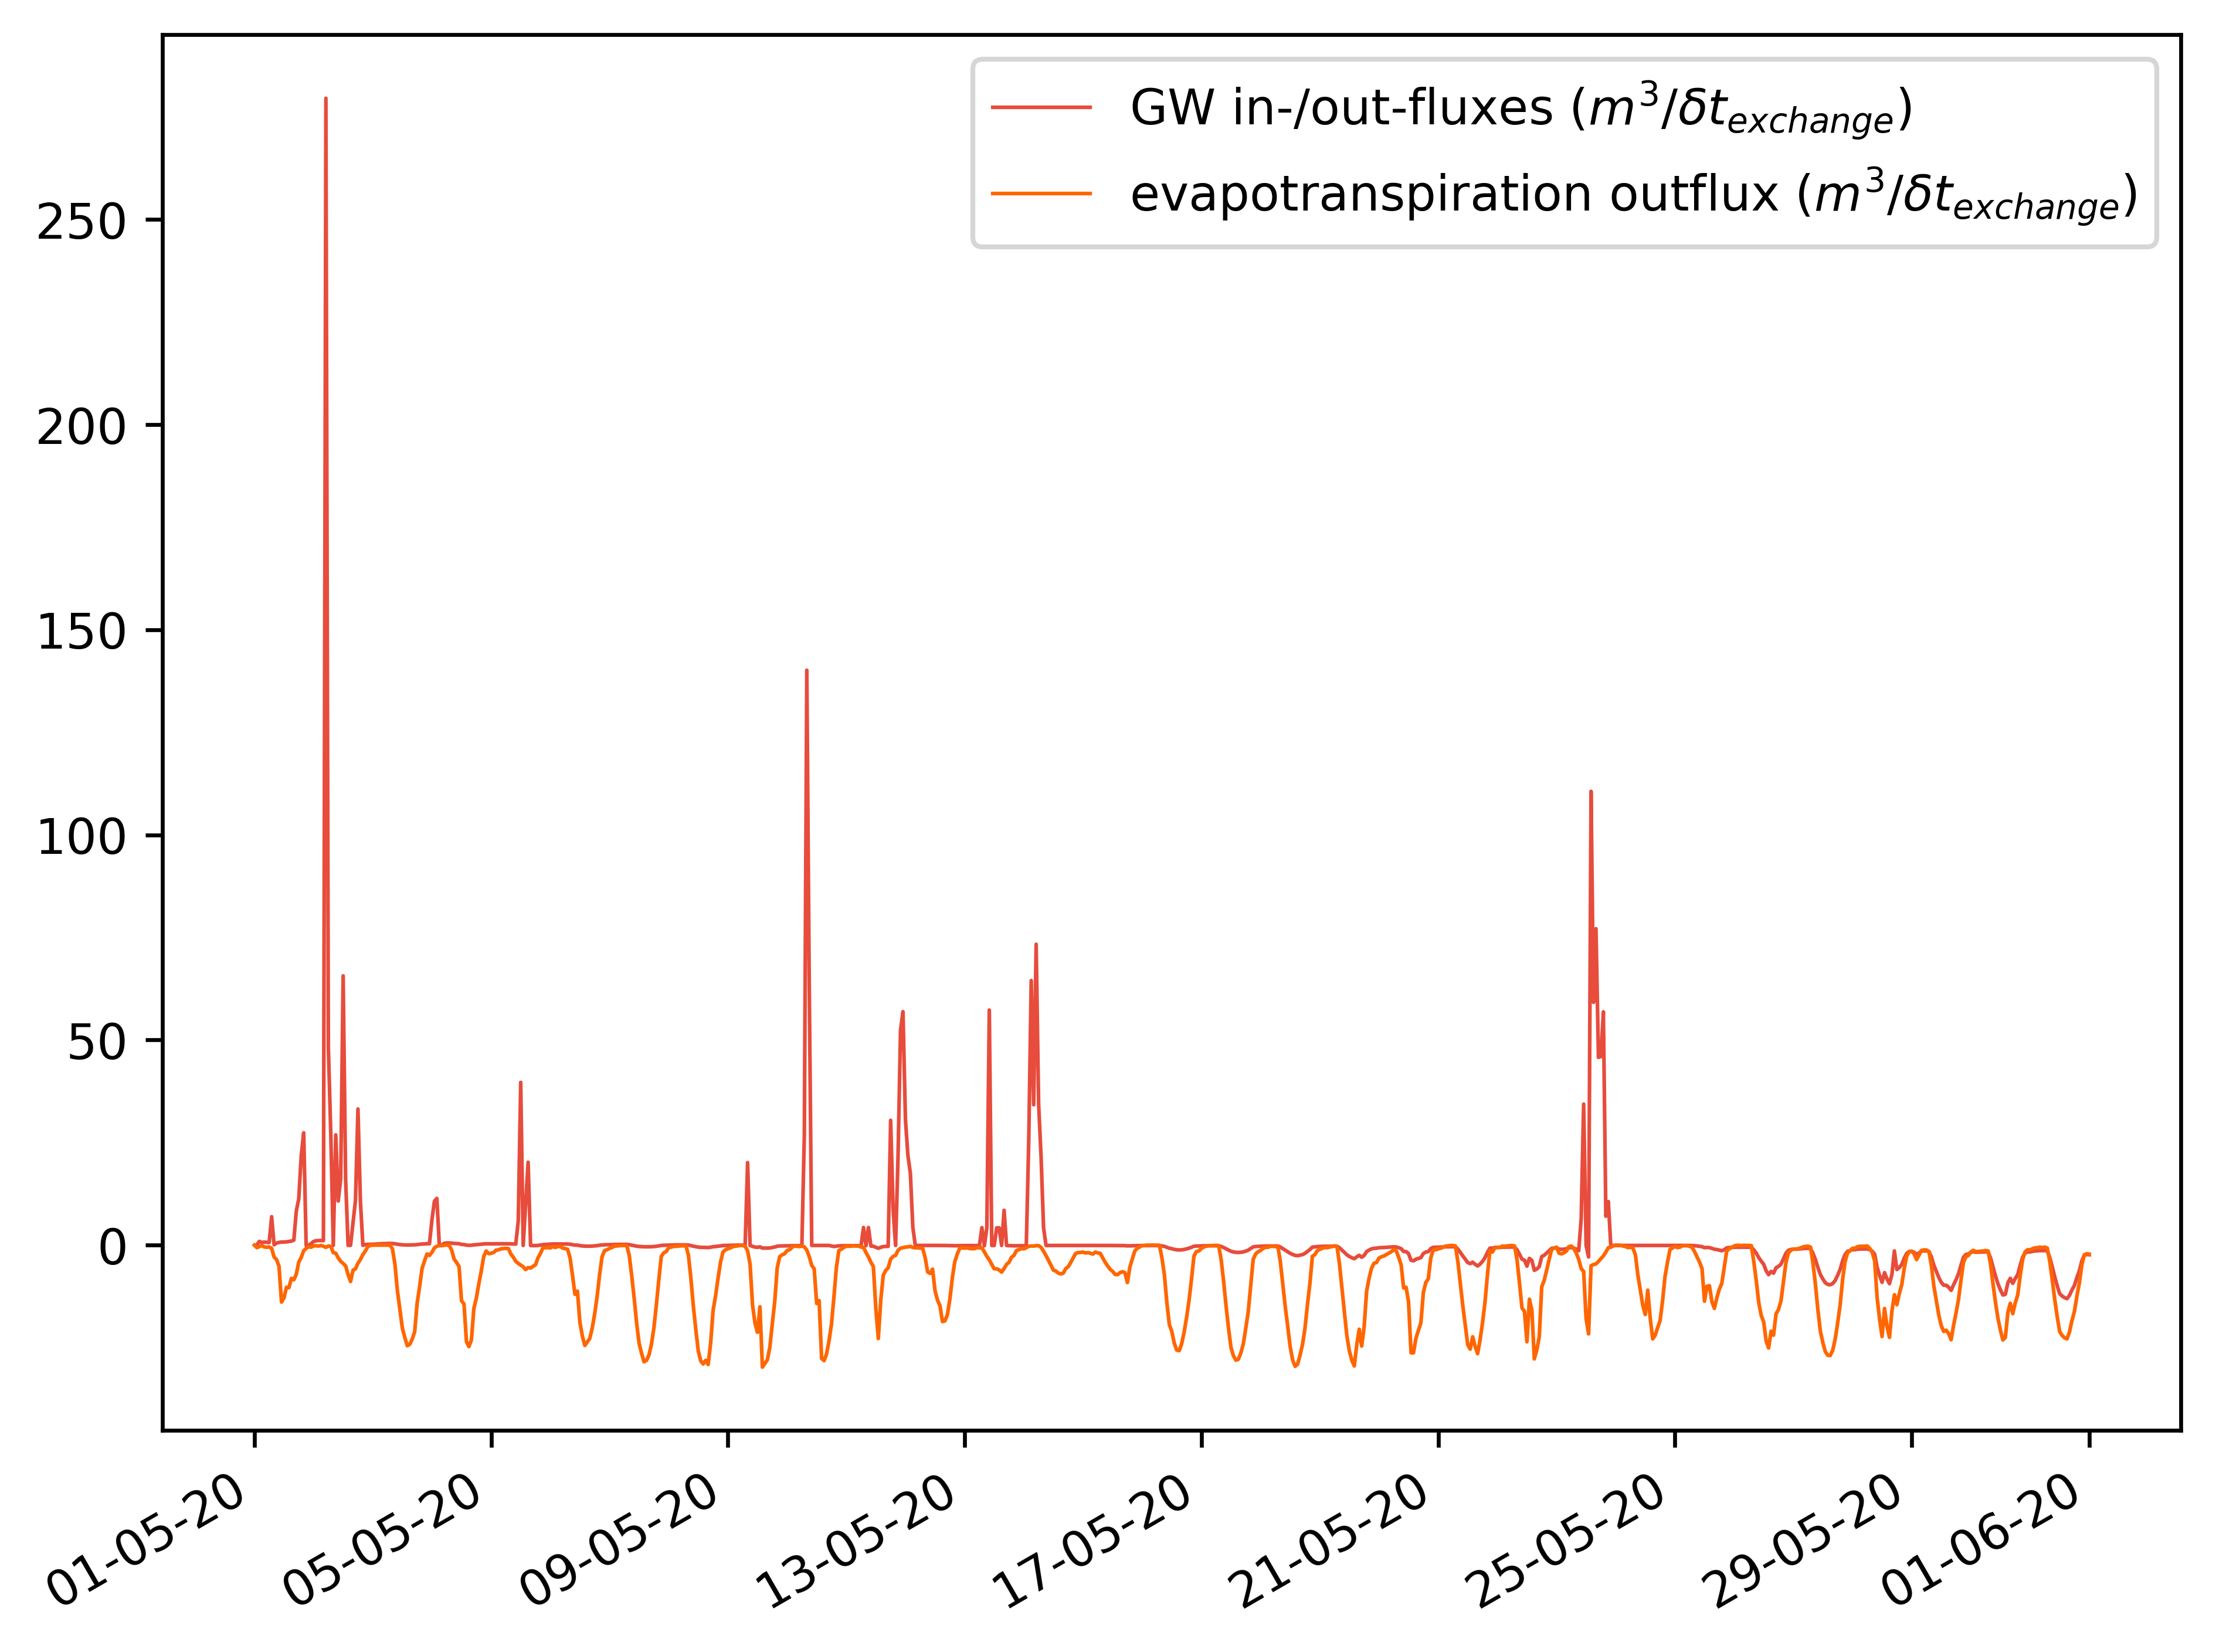
\includegraphics[height=0.42\textheight]{PICTURES/models_res/et_vs_gw}
    \caption{Comparing ET outfluxes with GW storage changes.}
    \label{fig:et_vs_gw}
\end{figure}
\begin{figure}[H]
    \centering
    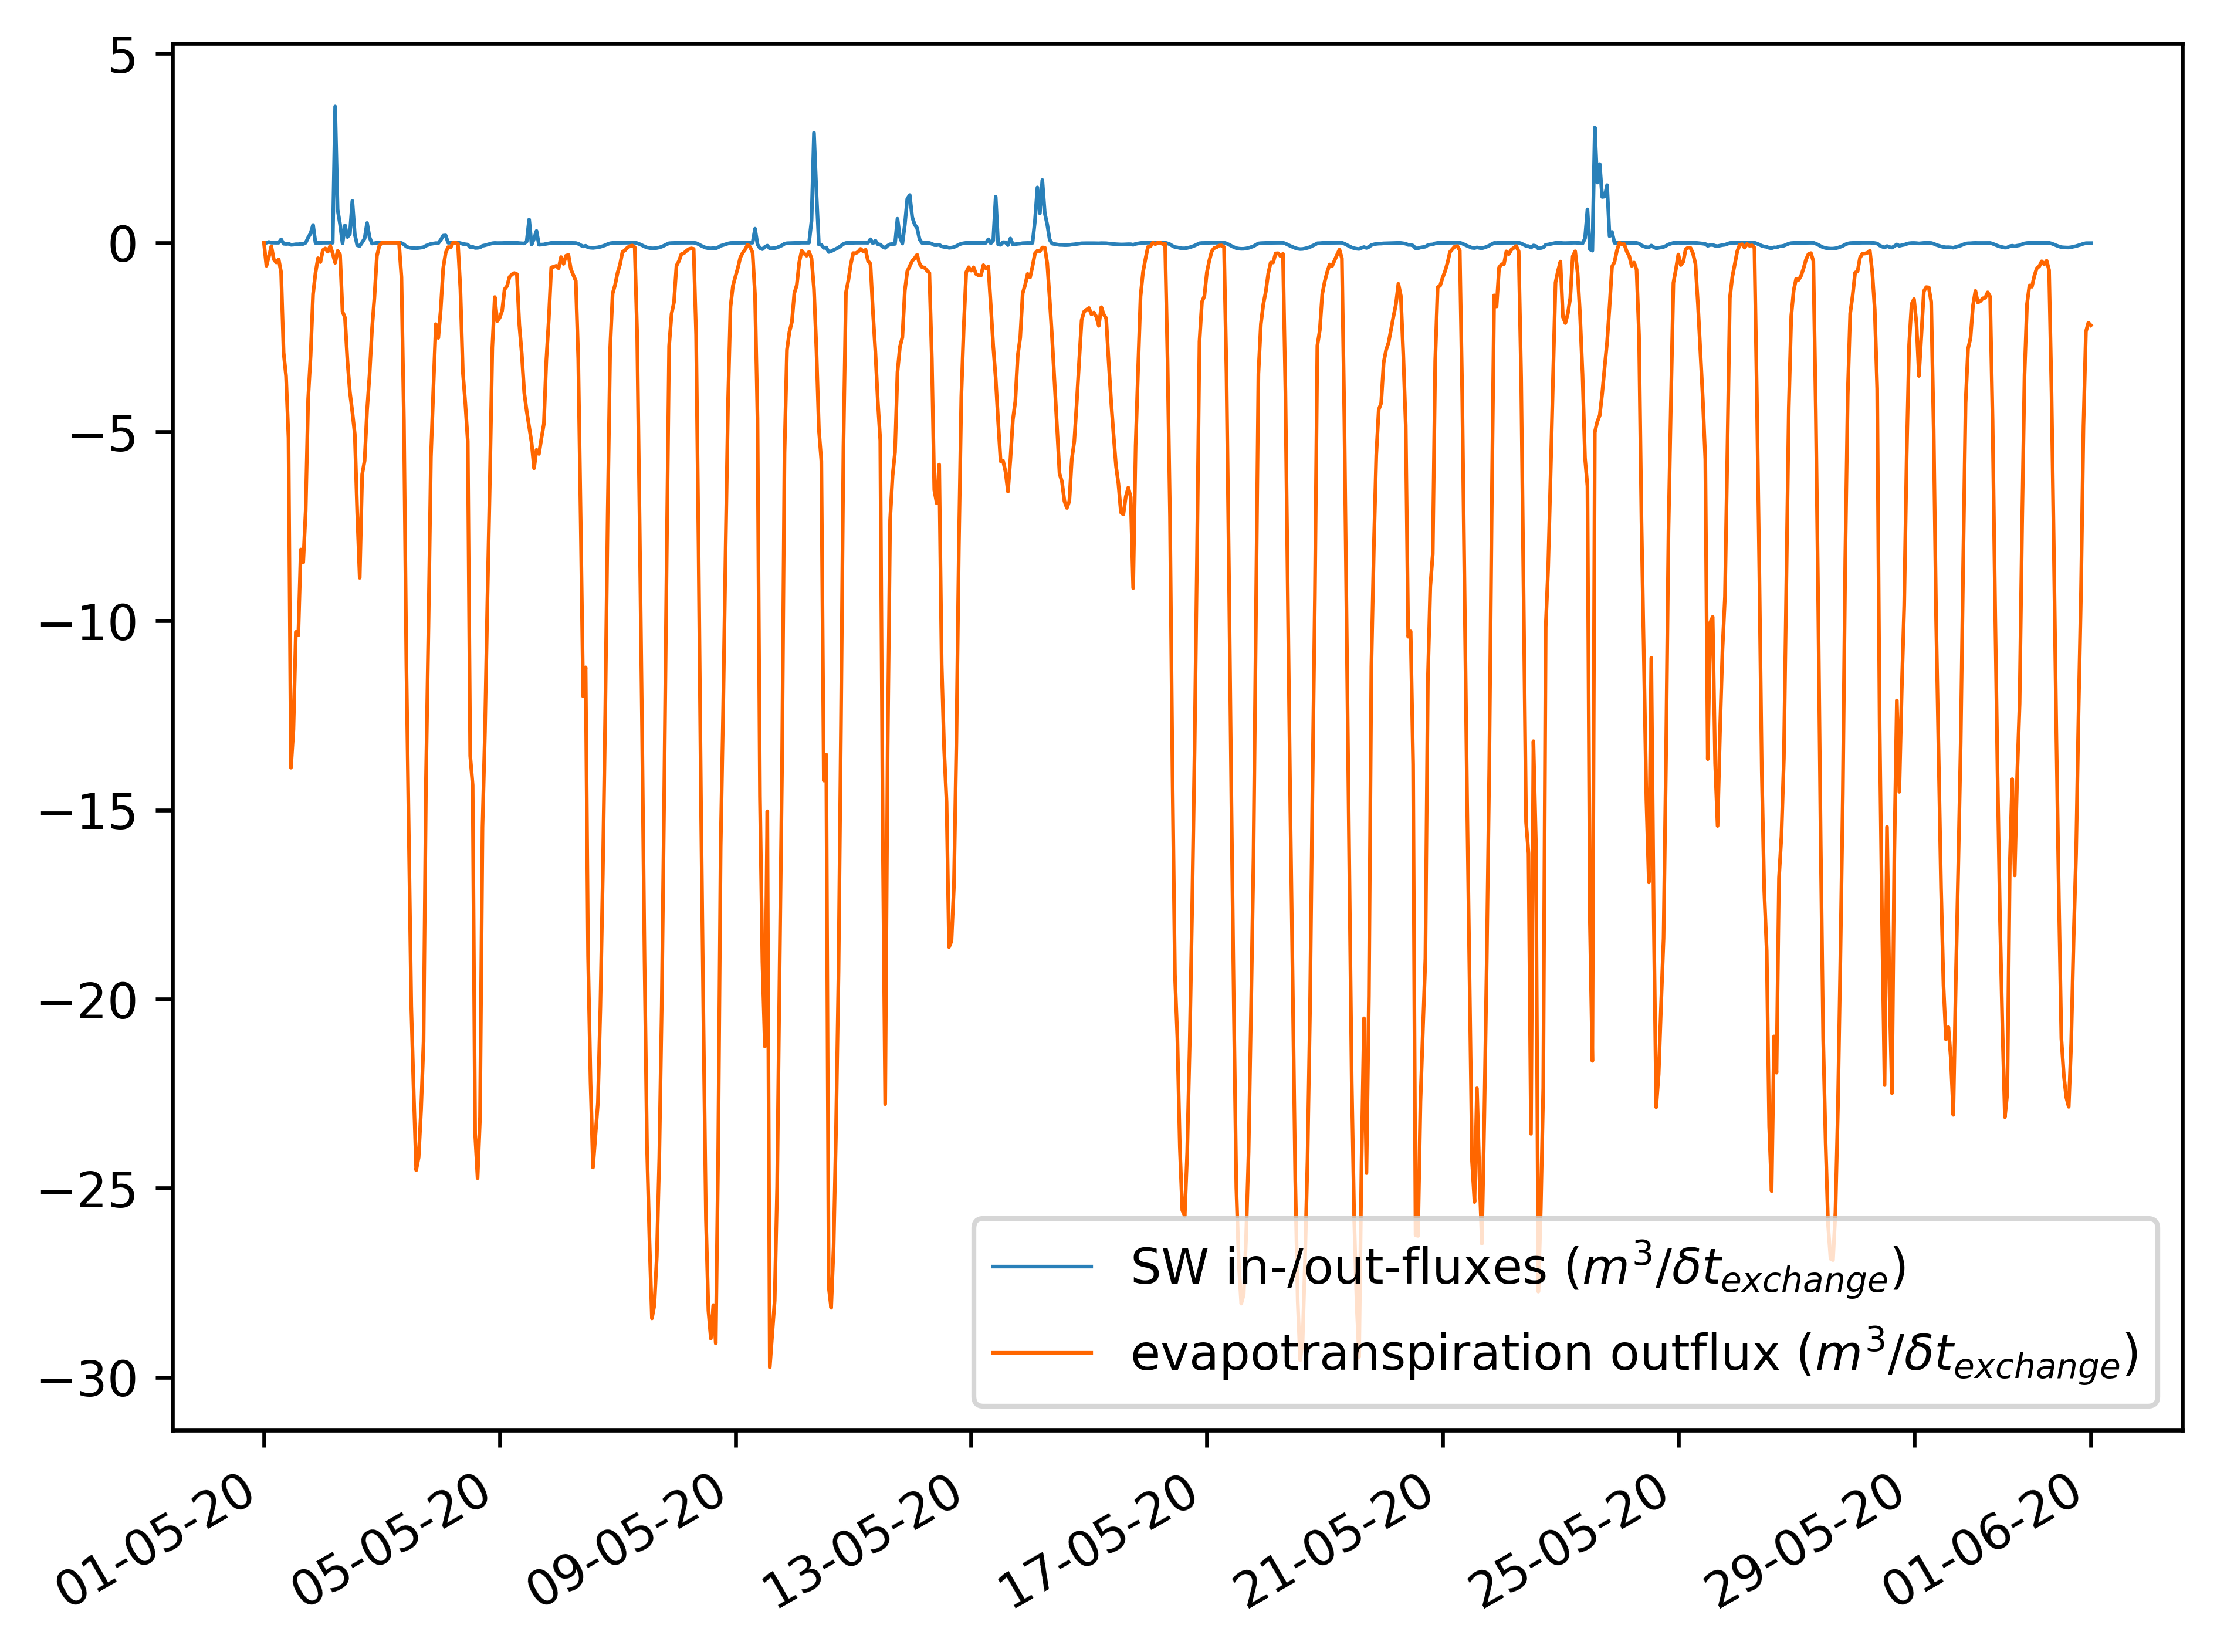
\includegraphics[width=\linewidth]{PICTURES/models_res/et_vs_sw}
    \caption{Comparing ET outfluxes with SW storage changes.}
    \label{fig:et_vs_sw}
\end{figure}


\subsection{Following Precipitation Influx}
The following plots follow the translation of precipitation influx into storage changes.
\\ \\
As seen from Figure \ref{fig:p_vs_gw}, a major portion of the precipitation influx is consistently translated into an influx into the GW storage. The model parameters that control the nature of this translation are $k$ and $\alpha$. Additionally, the SM storage in the previous time-step strongly defines this translation. While $k$ controls the maximum allowable rate of influx into the GW storage, $\alpha$ controls the non-linearity of the influx as discussed in Section \ref{GWSWEX_vs_Richards}.
\\ \\
A good portion of the precipitation influx is translated into an influx into the SM storage term as well. The nature of this translation is defined by the model parameters $\beta$, $n$, and $m$. Furthermore, it is also strongly defined by the SM storage in the previous time-step. While $\beta$ controls the non-linearity, $n$ defines the maximum allowable SM storage, and $m$ defines $SM_\textrm{min}$, beyond which the SM storage is not reducible, as discussed in Section \ref{GWSWEX_vs_Richards}.
\\ \\
As was expected for this simulation period, not much of the precipitation influx was translated into influxes to the SW storage term. The nature of this translation is controlled by the nature of translations of precipitation influxes into the GW and SM terms, as discussed in \ref{fig:GWSWEX_flow}.

\begin{figure}[H]
\centering
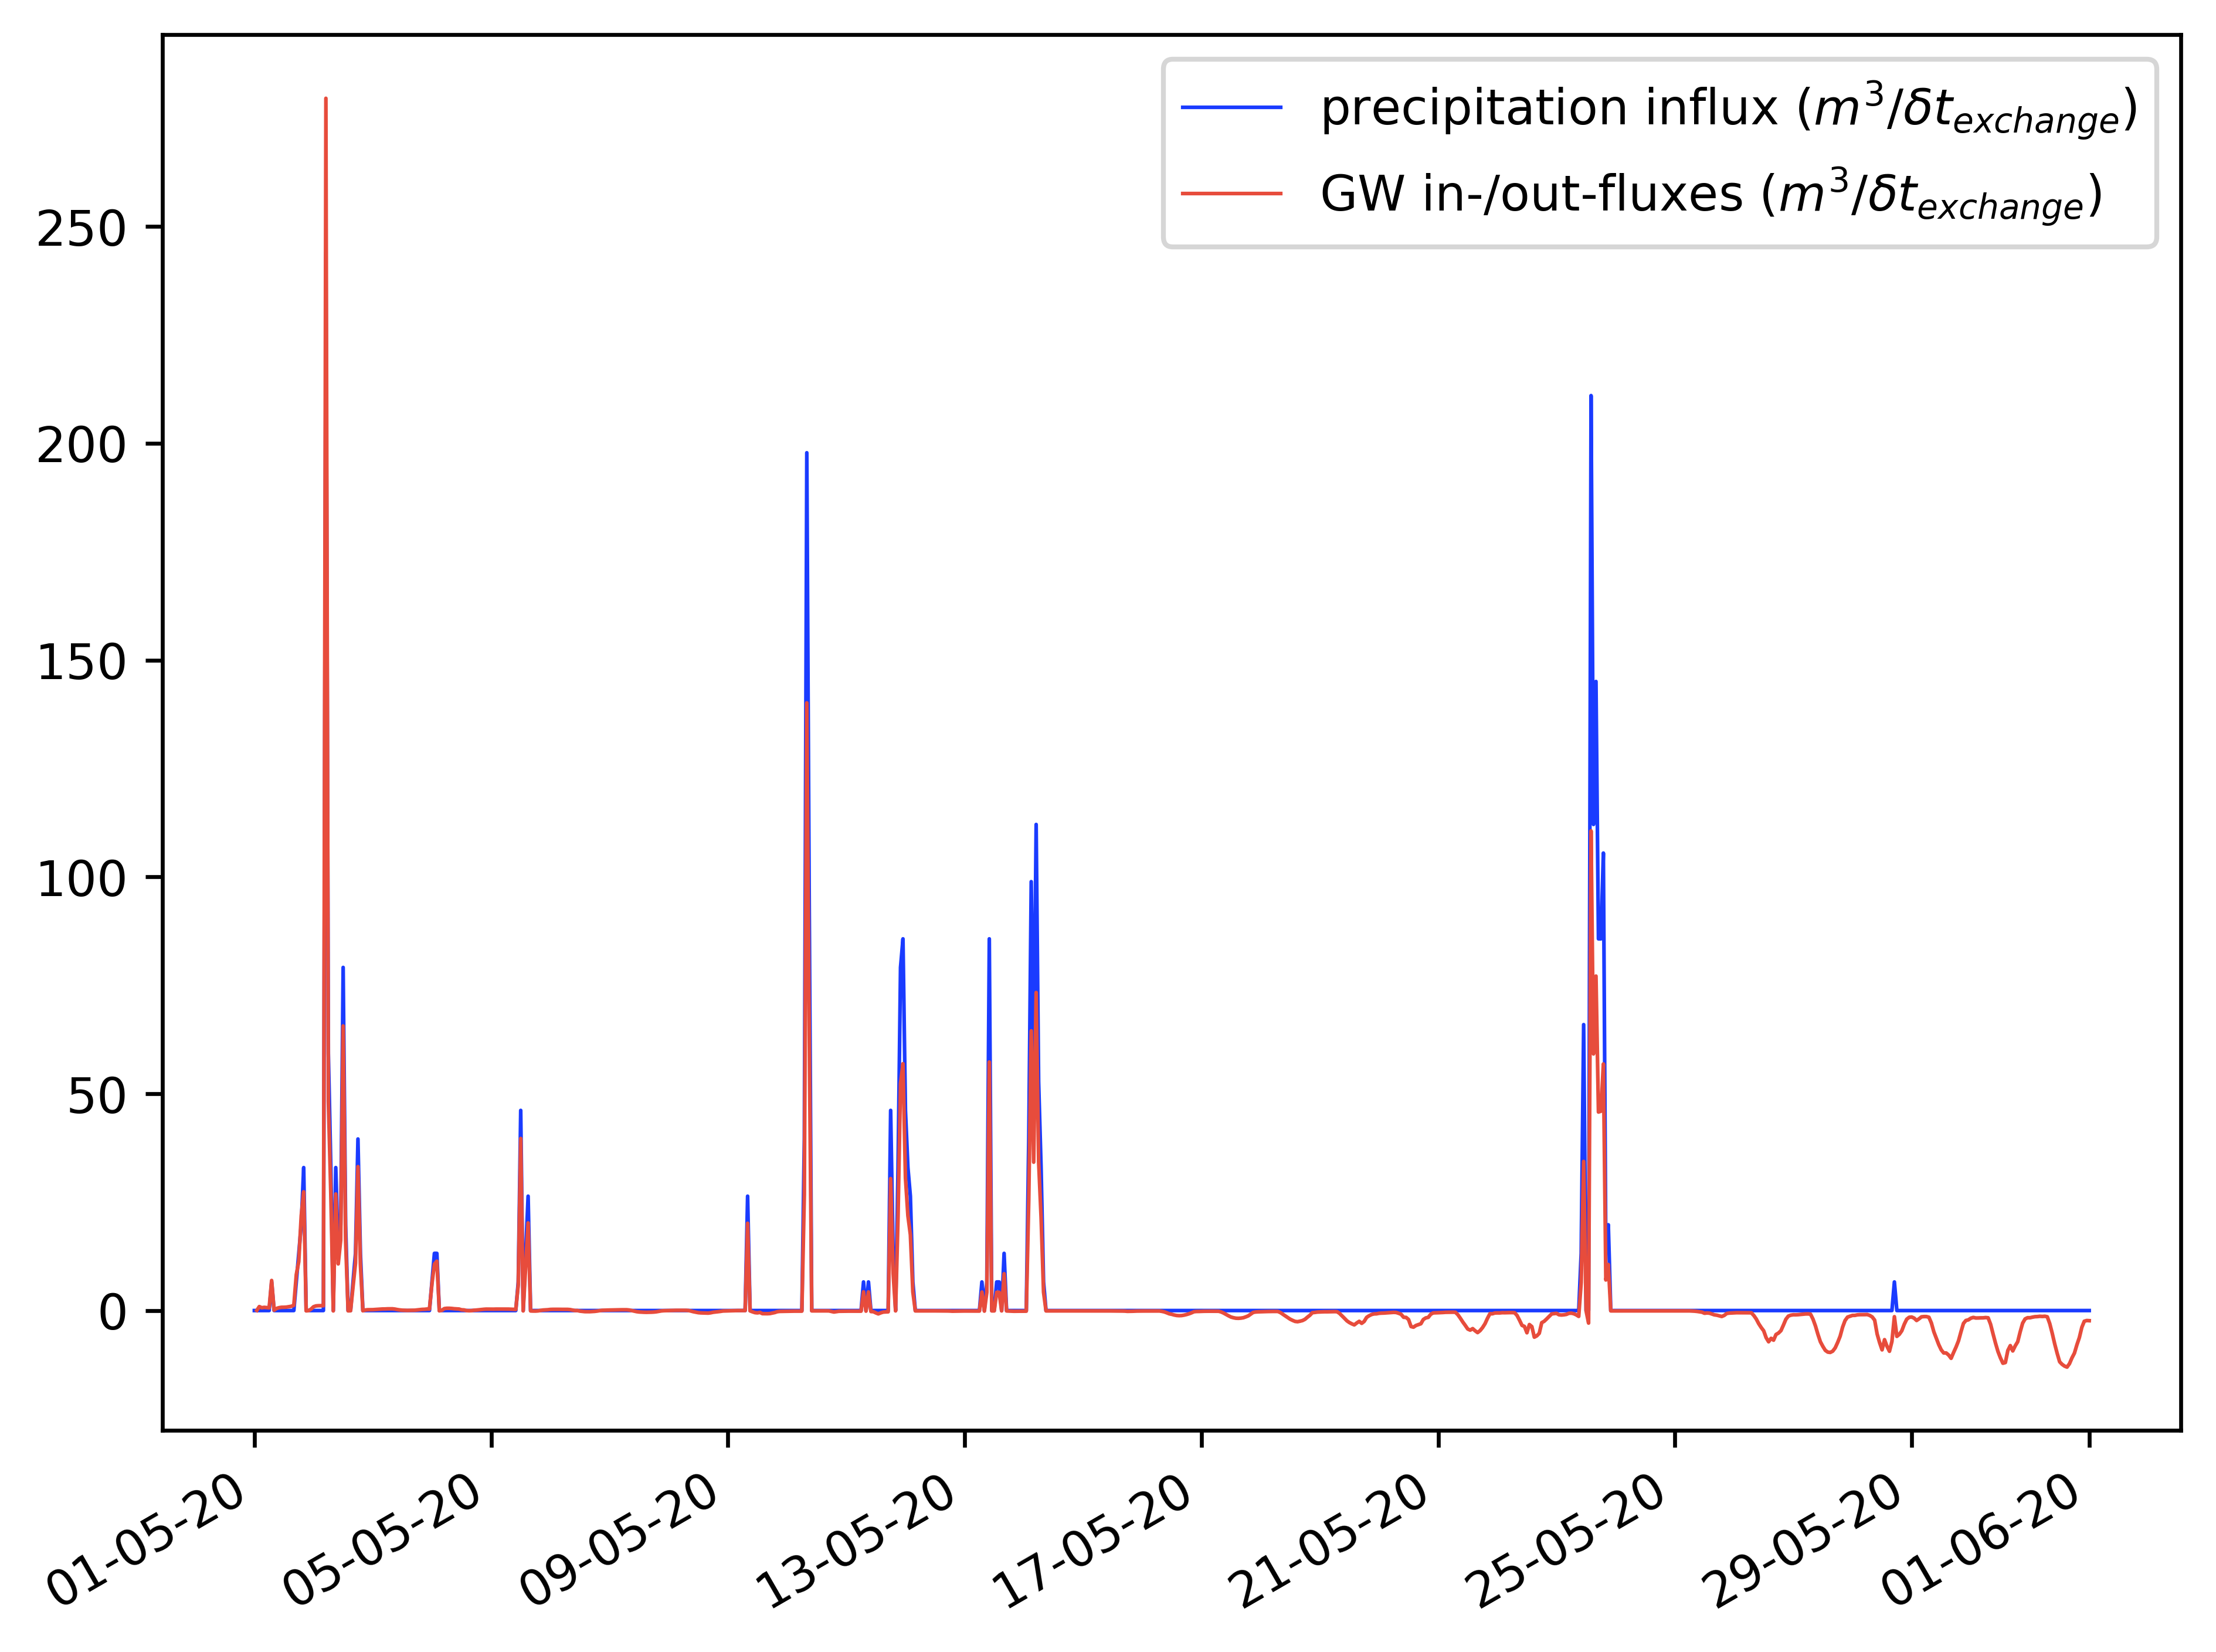
\includegraphics[width=\linewidth]{PICTURES/models_res/p_vs_gw}
\caption{Comparing P influxes with GW storage changes.}\label{fig:p_vs_gw}
\end{figure}
\begin{figure}[H]
\centering
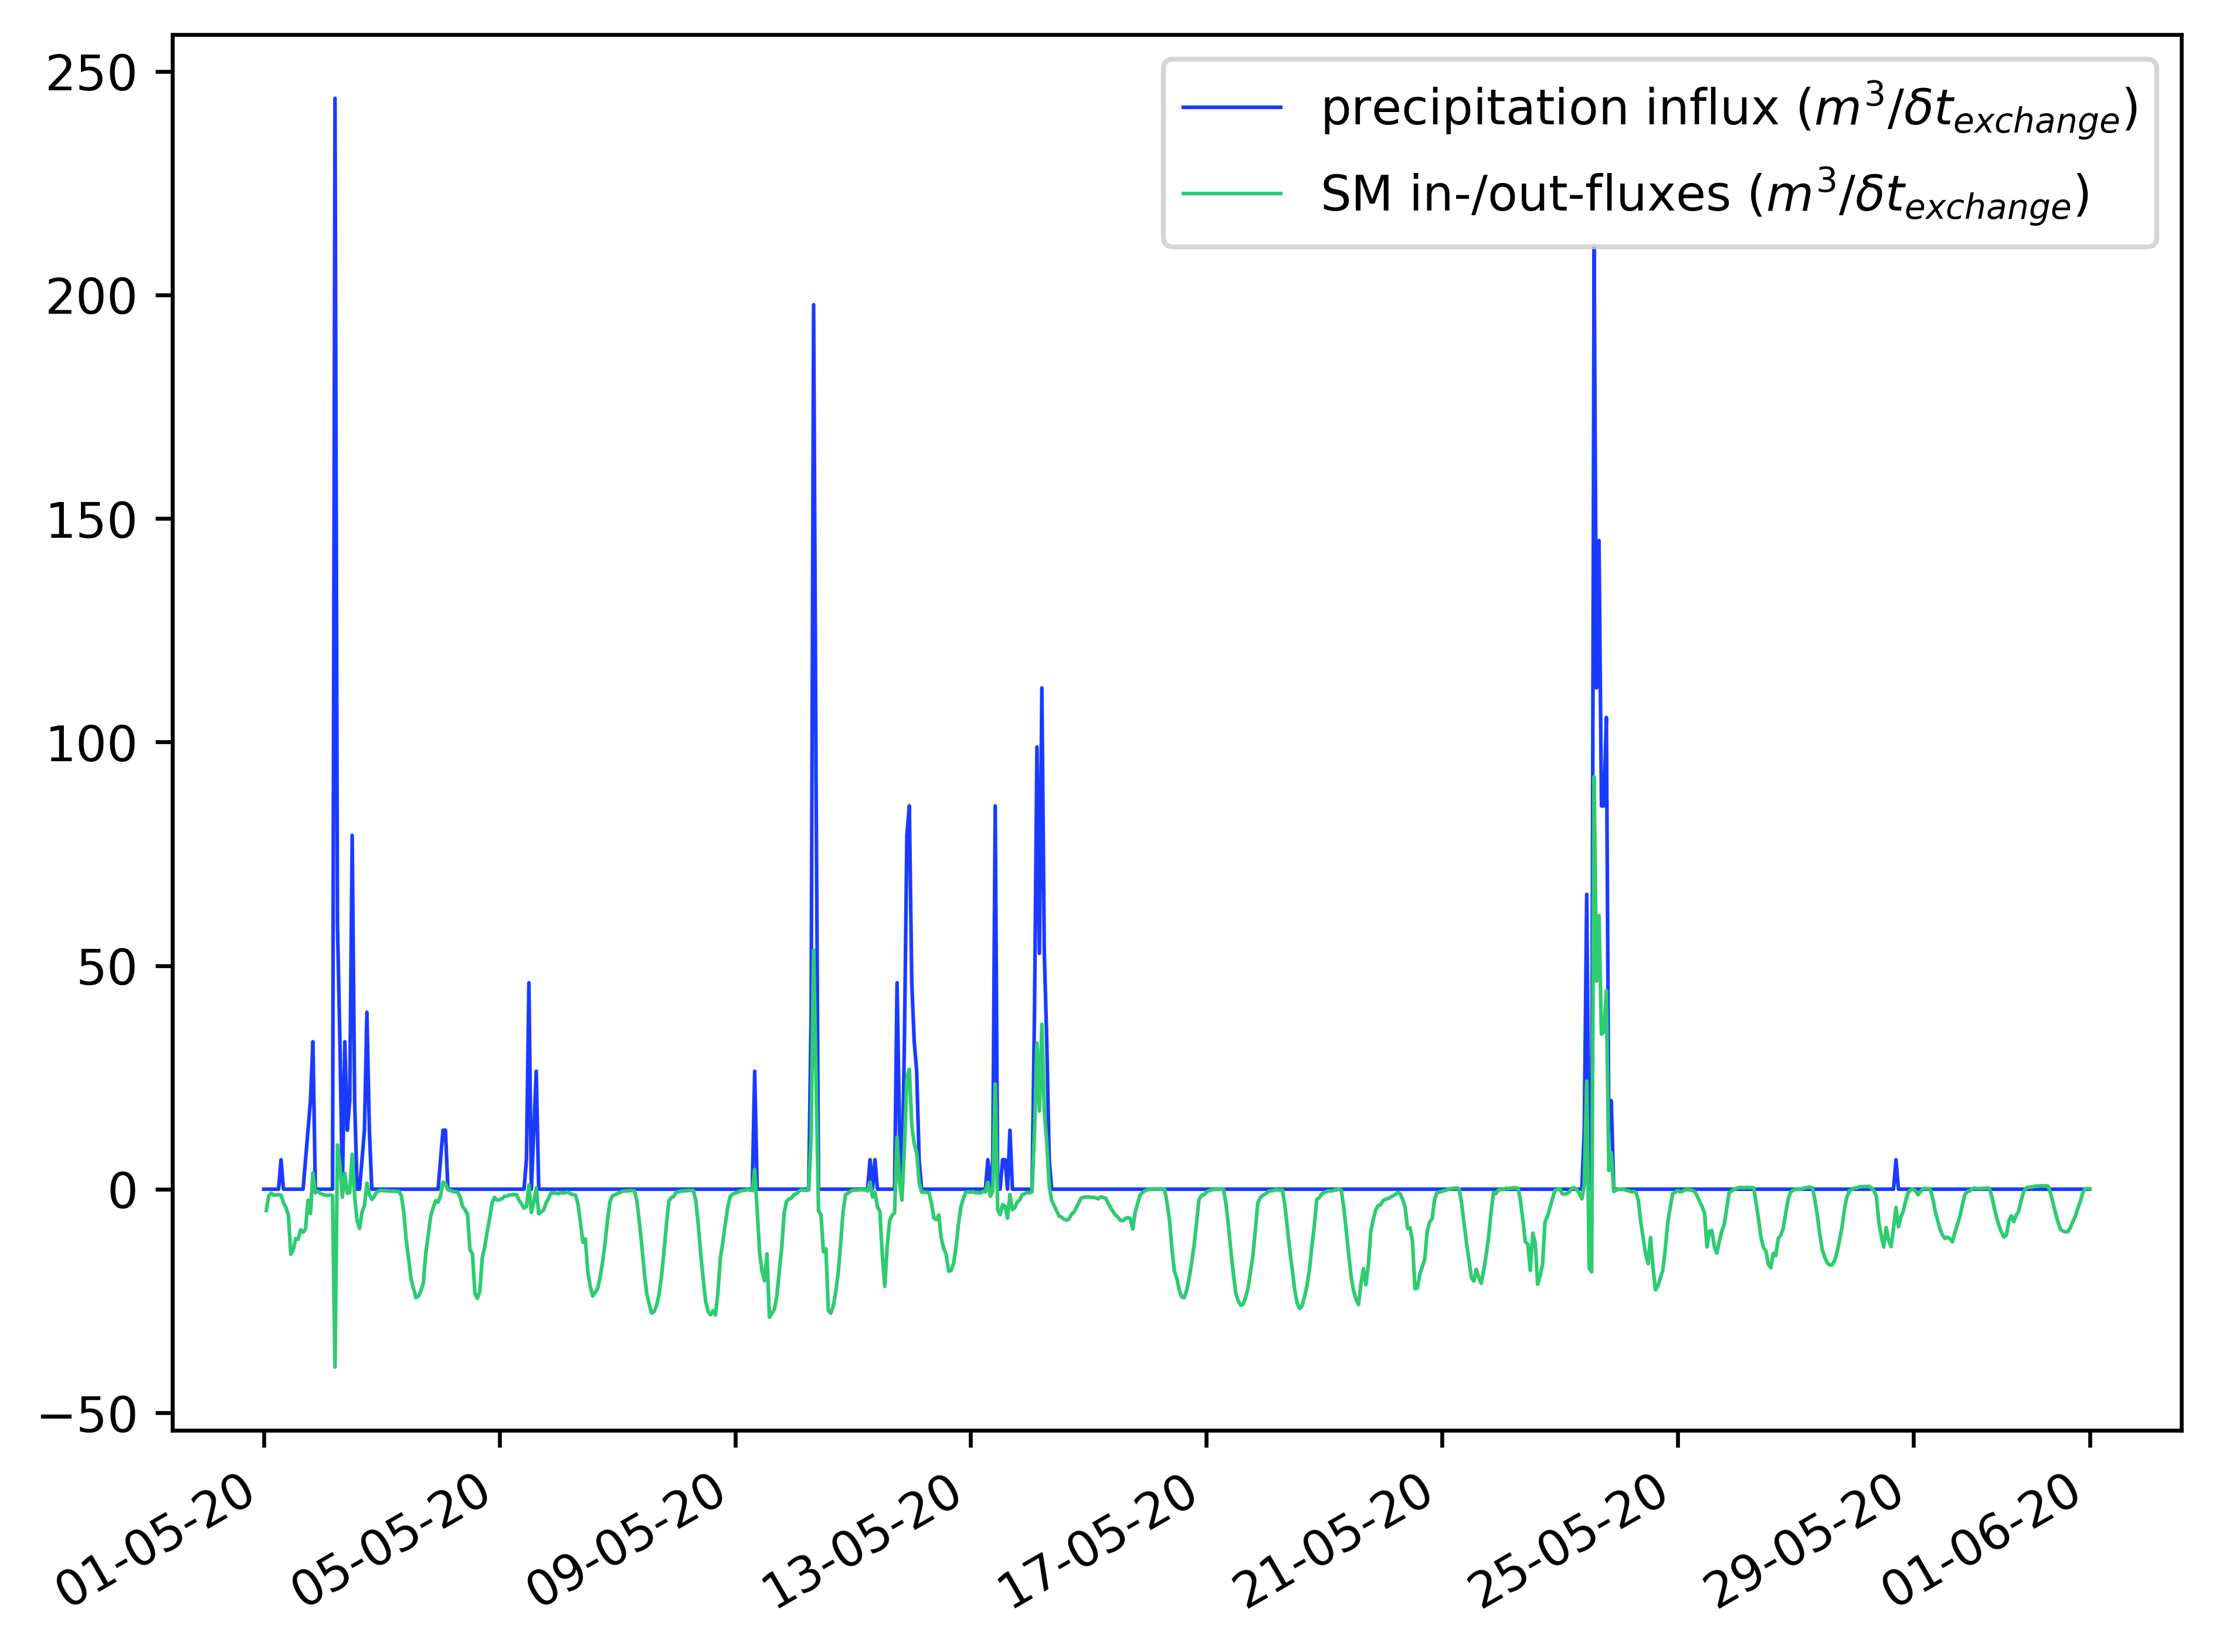
\includegraphics[height=0.42\textheight]{PICTURES/models_res/p_vs_sm}
\caption{Comparing P influxes with SM storage changes.}\label{fig:p_vs_sm}
\end{figure}
\begin{figure}[H]
\centering
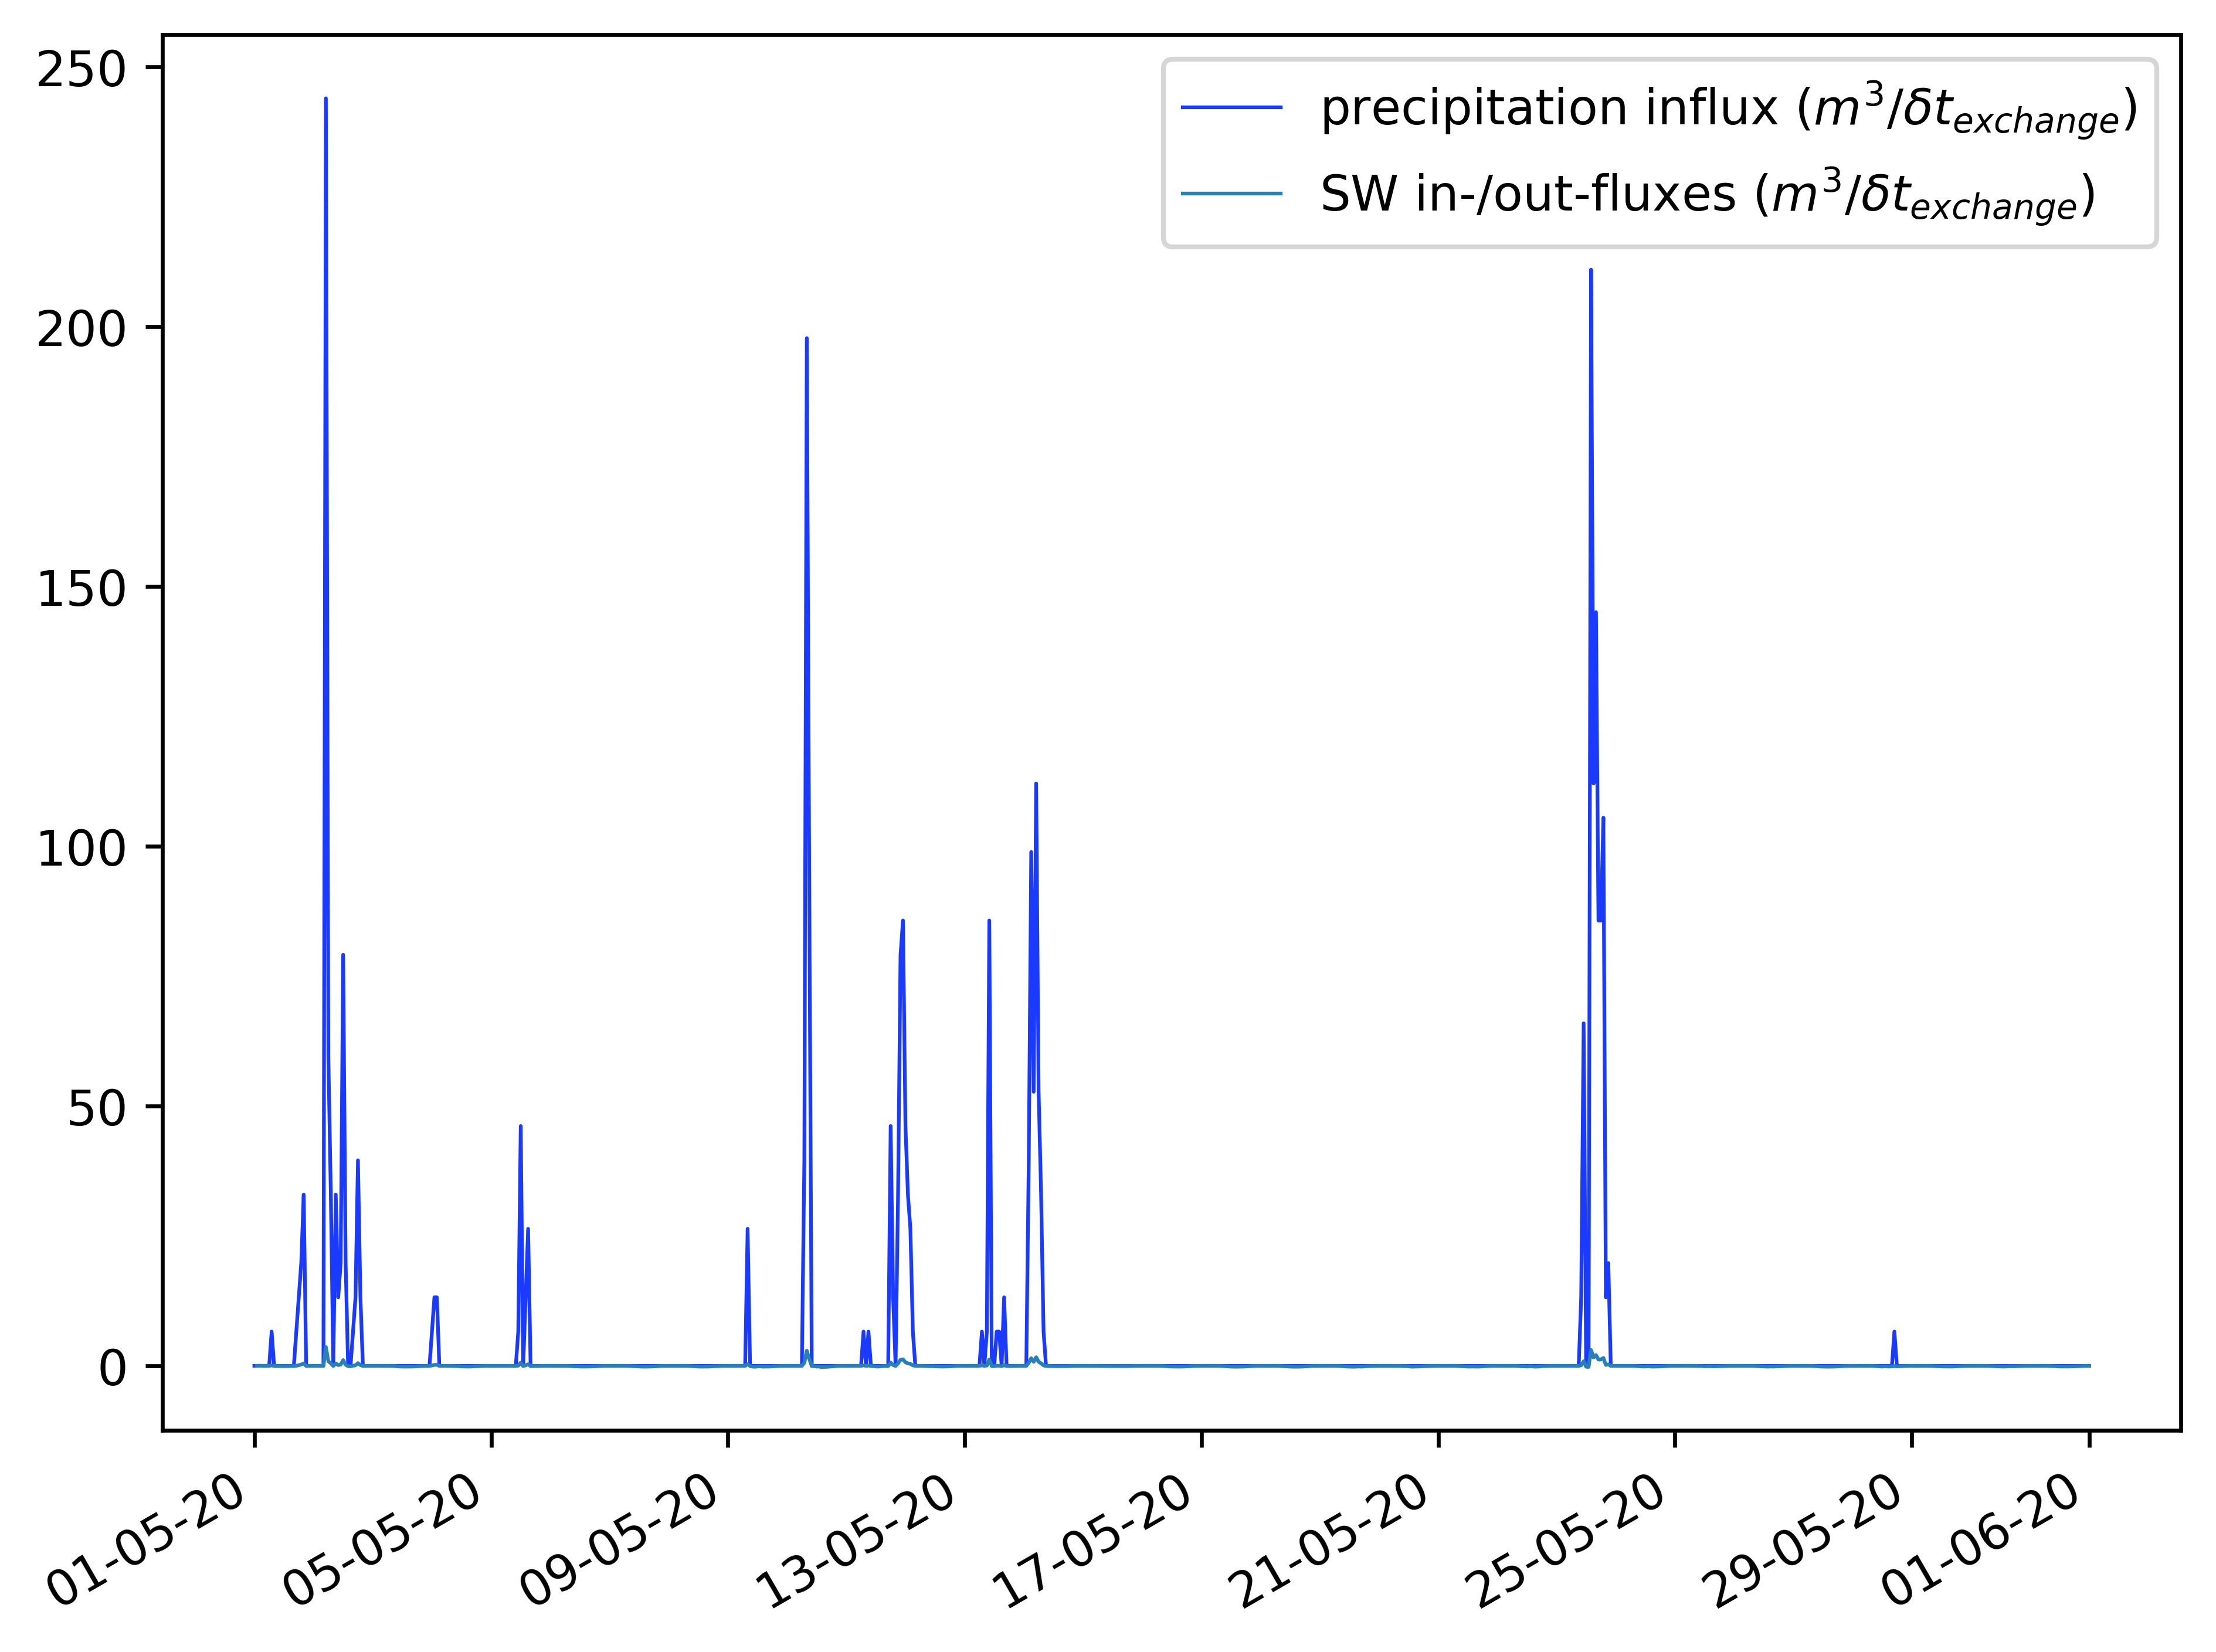
\includegraphics[height=0.42\textheight]{PICTURES/models_res/p_vs_sw}
\caption{Comparing P influxes with SW storage changes.}\label{fig:p_vs_sw}
\end{figure}

\subsection{Following GW and SM Fluxes}
As discussed in \ref{fig:GWSWEX_flow}, an increase in GW levels imply a reduction in the unsaturated zone and thus the effective pore volume in the unsaturated zone. From this, it is to be expected that a considerable influx into the GW storage must imply a considerable outflux from the SM storage. This may be observed in Figure \ref{fig:sm_vs_gw}.
\begin{figure}[H] 
\centering
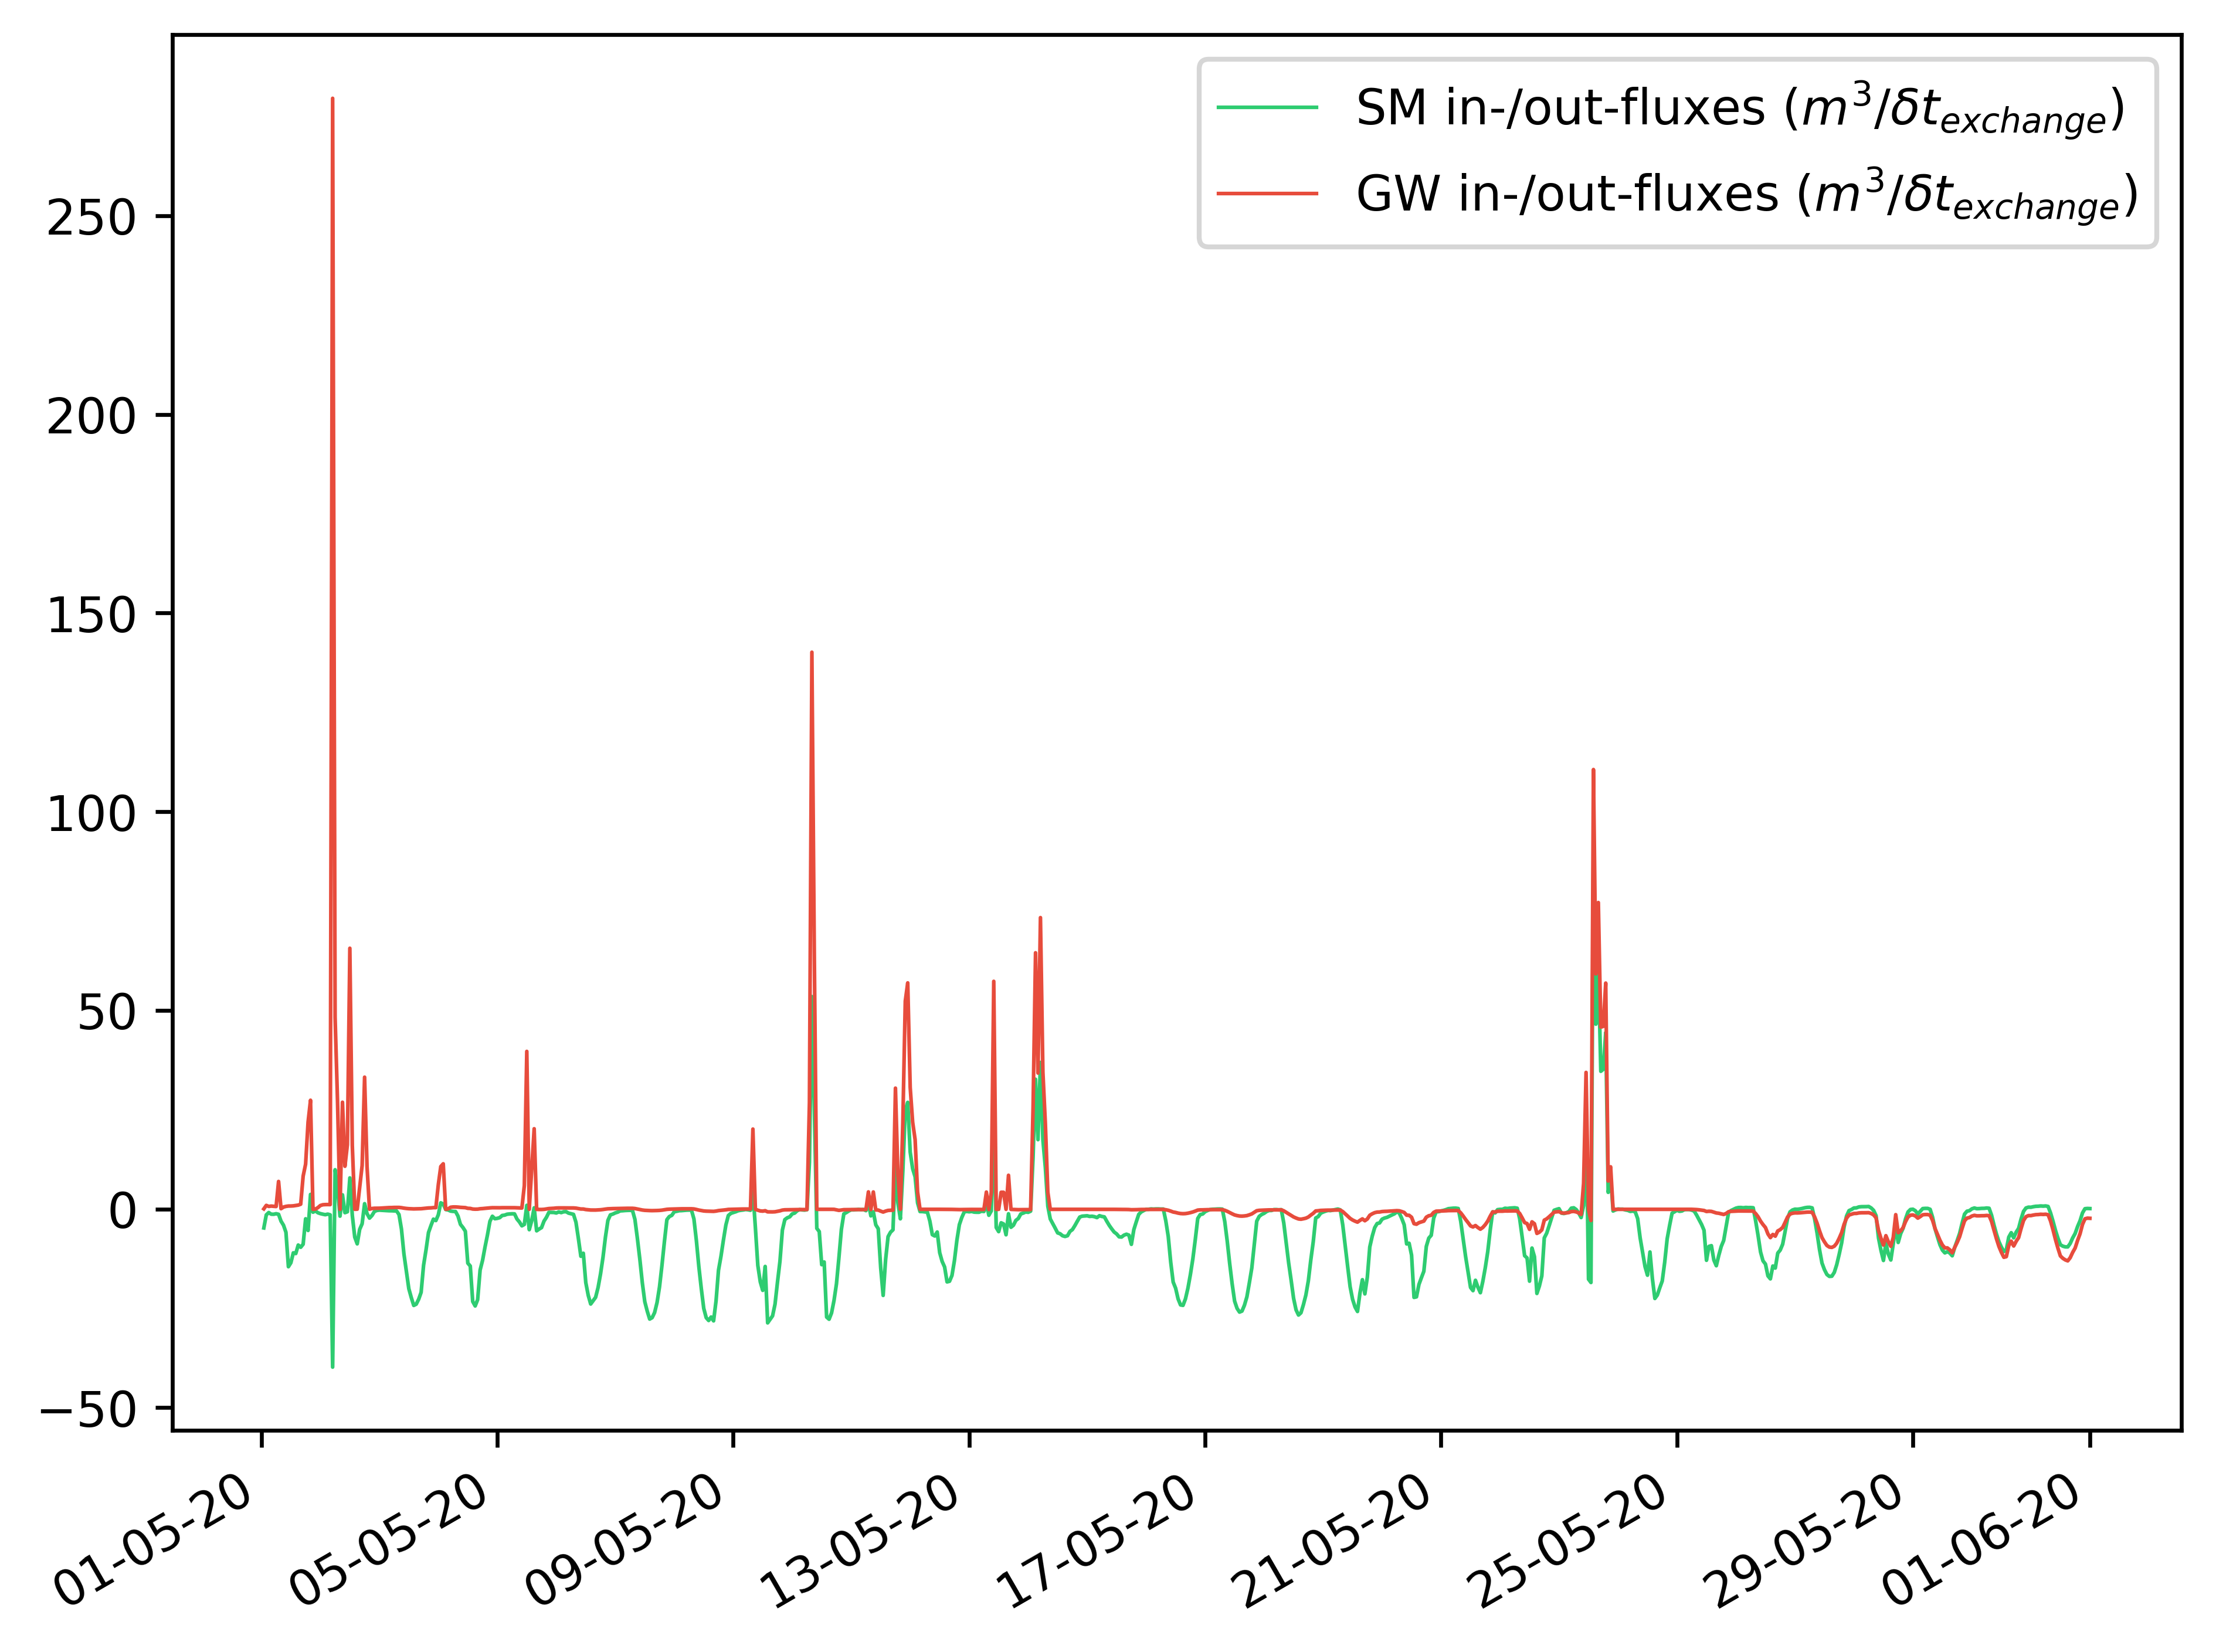
\includegraphics[height=0.42\textheight]{PICTURES/models_res/sm_vs_gw}
\caption{Comparing SM and GW storage changes.}\label{fig:sm_vs_gw}
\end{figure}
Further, to maintain $SM_\textrm{min}$, there outflux from GW is translated into influx into SM, as seen in Figures \ref{fig:sm_vs_gw}, \ref{fig:p_vs_gw}, and \ref{fig:p_vs_sm} starting roughly from 26-05-2020 to the end of the simulation period.

\section{Storages}
Figure \ref{fig:mf6_res} shows the hydraulic heads in the GW model at the end of the simulation. Comparing it with \ref{fig:mf6_ic_strt}, one may notice that the hydraulic heads in the unconfined aquifer has significantly decreased, owing to the dominance of ET outfluxes.
\\ \\
The dominant ET outfluxes have resulted in a reduction in the SM storage as well, as observed in \ref{fig:sm_res}. One may observe that the reduction in SM is stronger along the dewatering stream.

\begin{figure}[H]
\minipage{0.32\textwidth}
  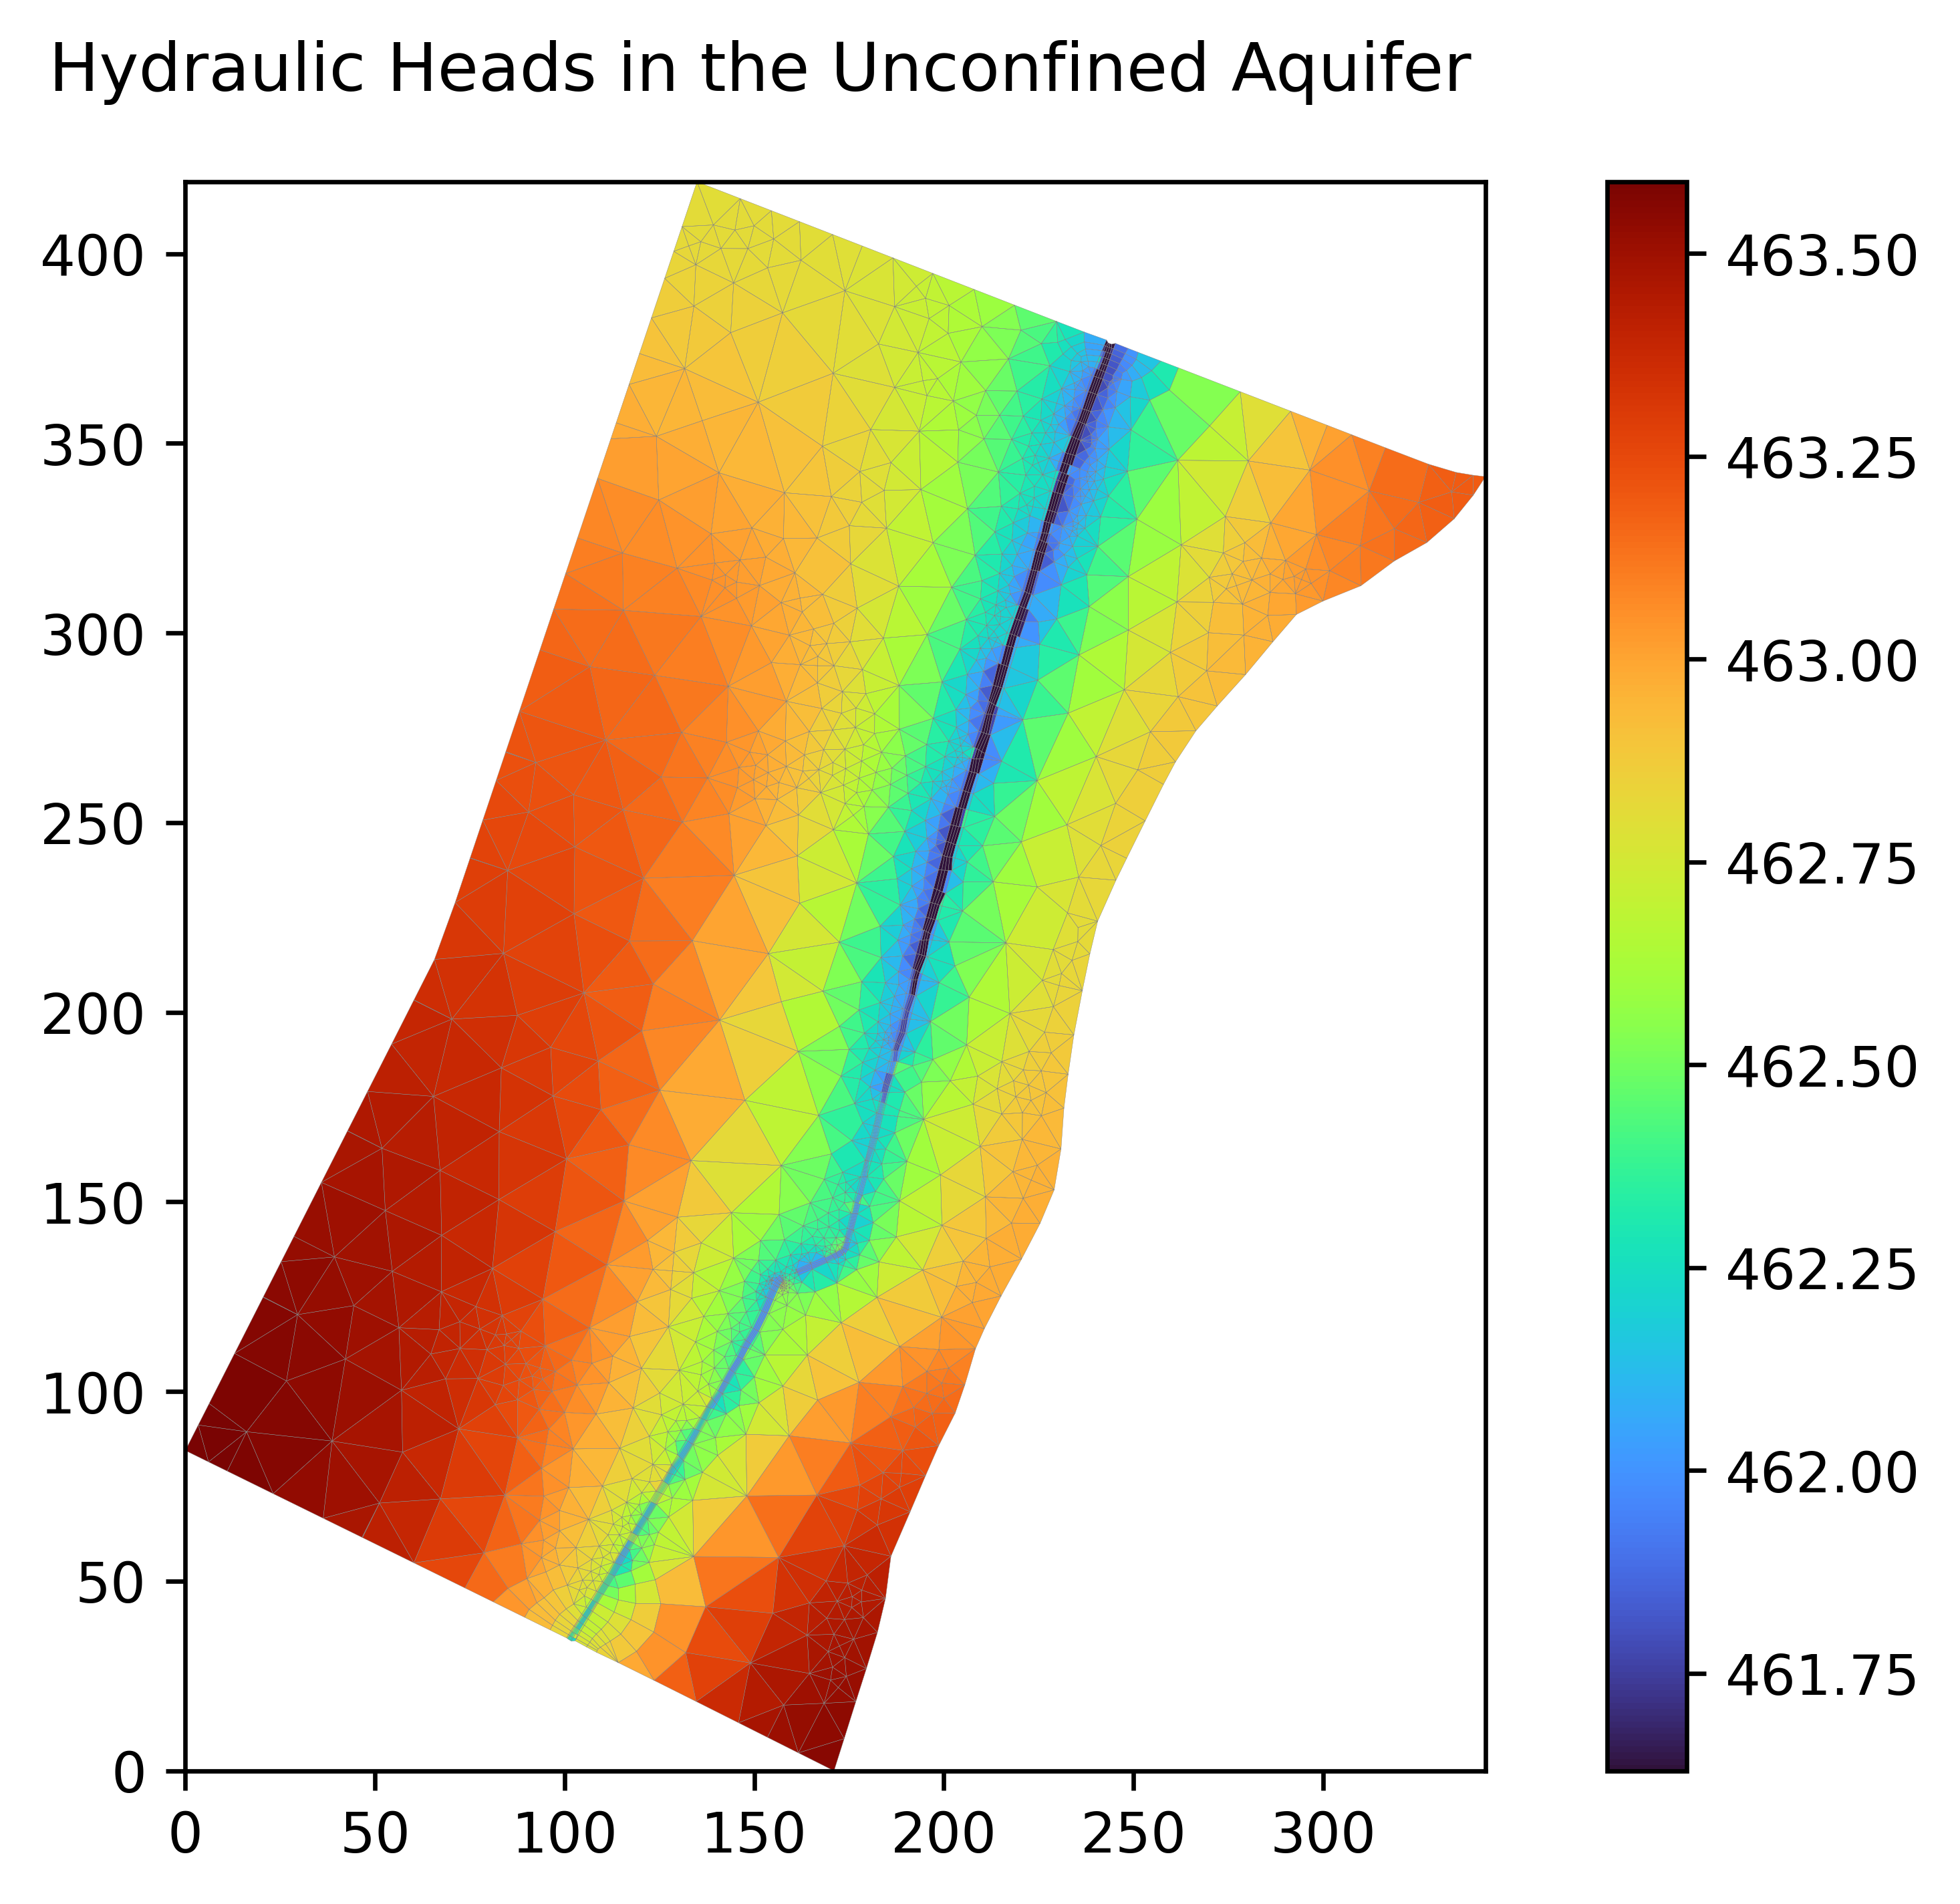
\includegraphics[width=\linewidth]{PICTURES/models_res/h_l1}
\endminipage\hfill
\minipage{0.32\textwidth}
  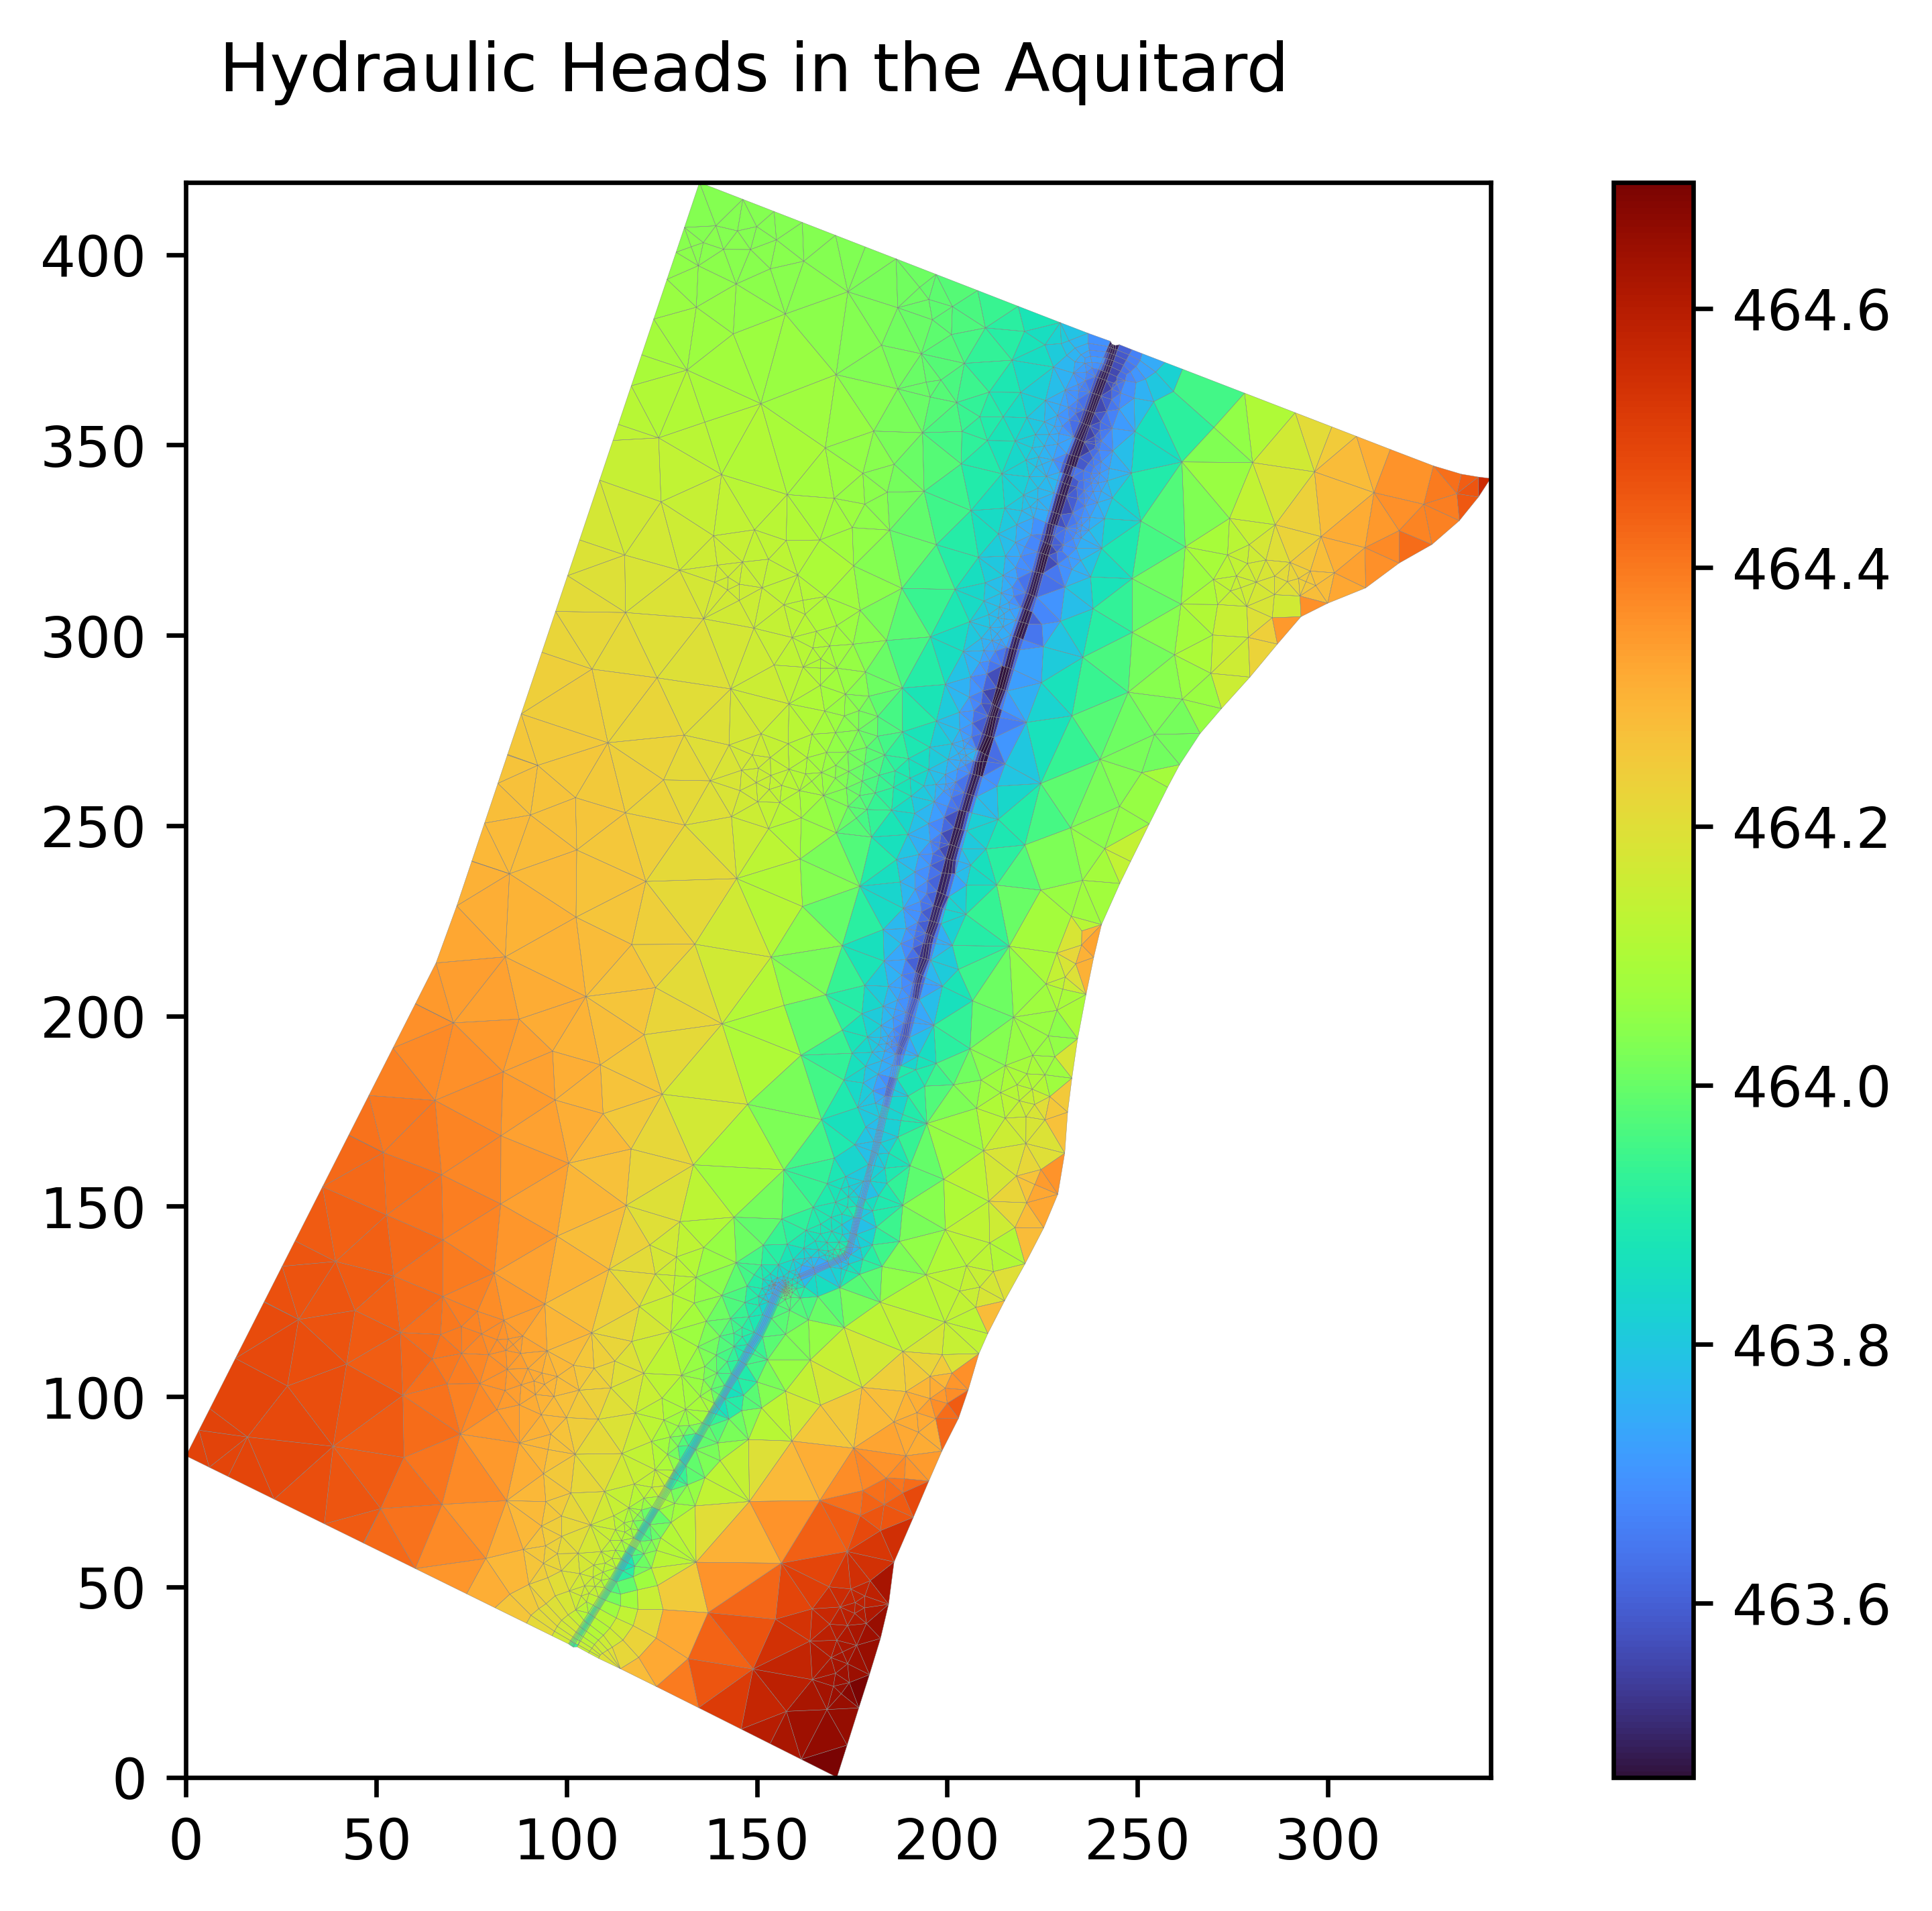
\includegraphics[width=\linewidth]{PICTURES/models_res/h_l2}
\endminipage\hfill
\minipage{0.32\textwidth}
  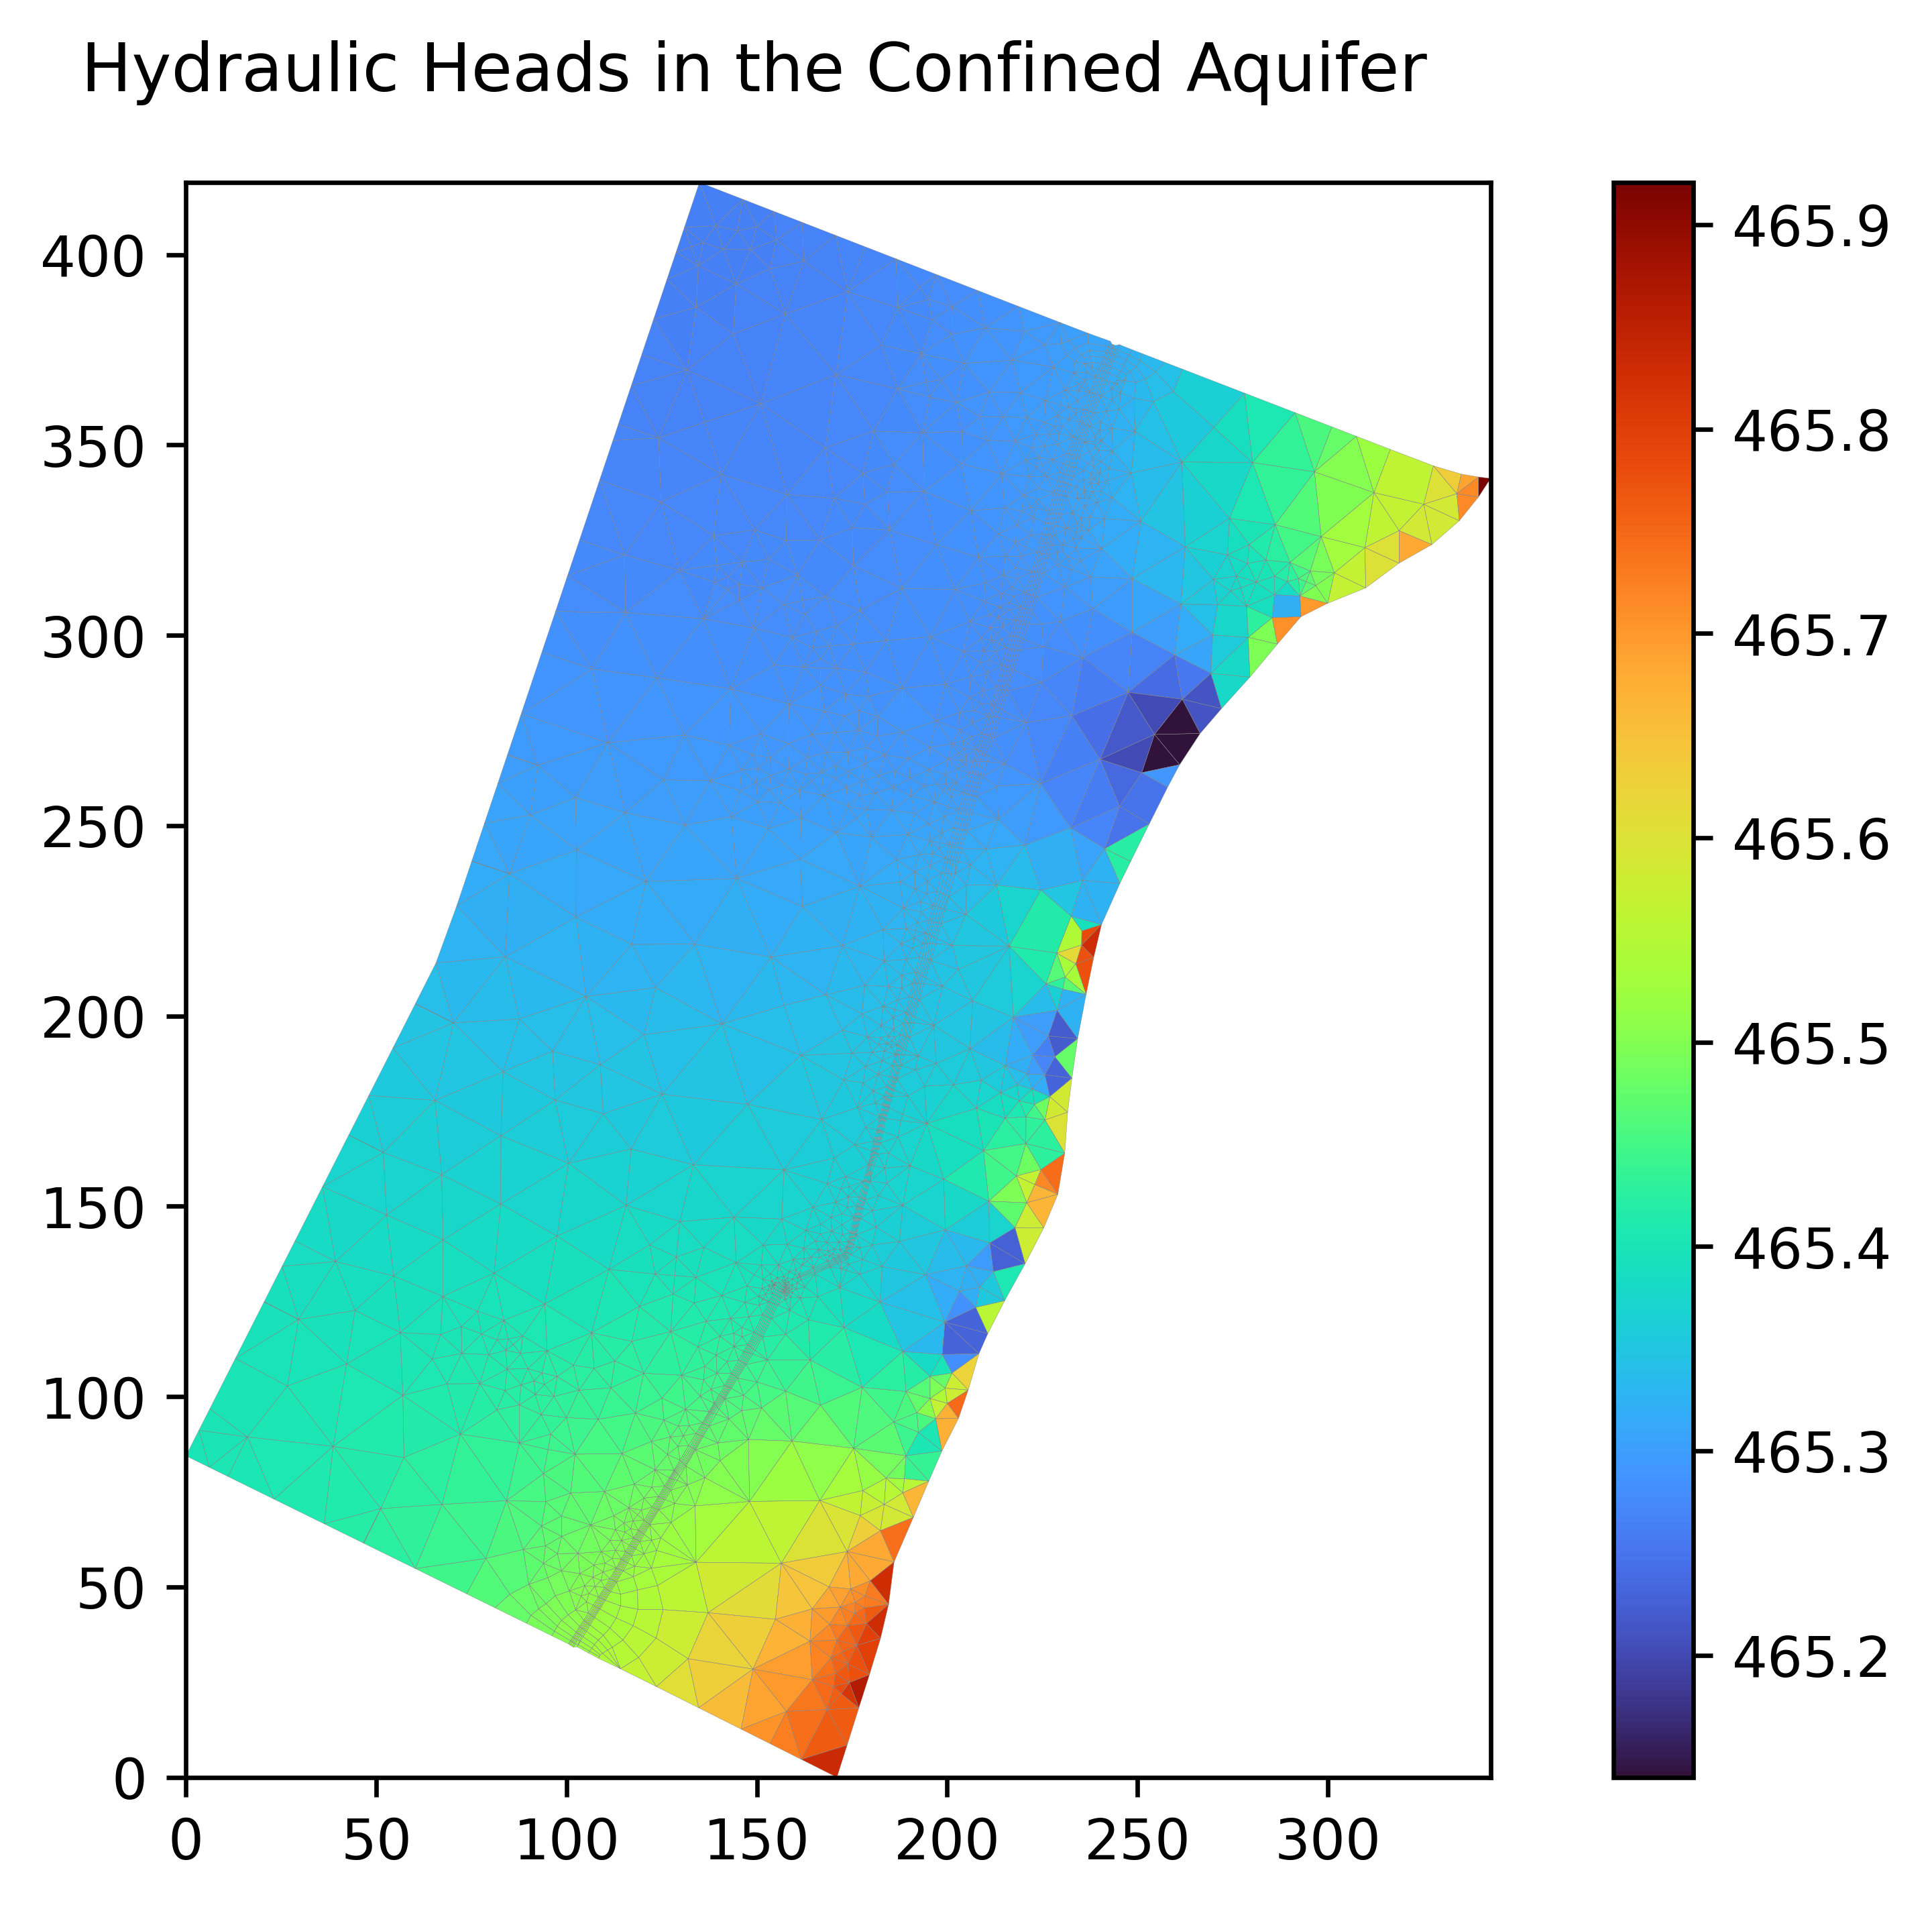
\includegraphics[width=\linewidth]{PICTURES/models_res/h_l3}
\endminipage
\caption{Starting heads in the GW Model.}\label{fig:mf6_res}
\end{figure}

\begin{figure}[H]
\minipage{0.5\textwidth}
  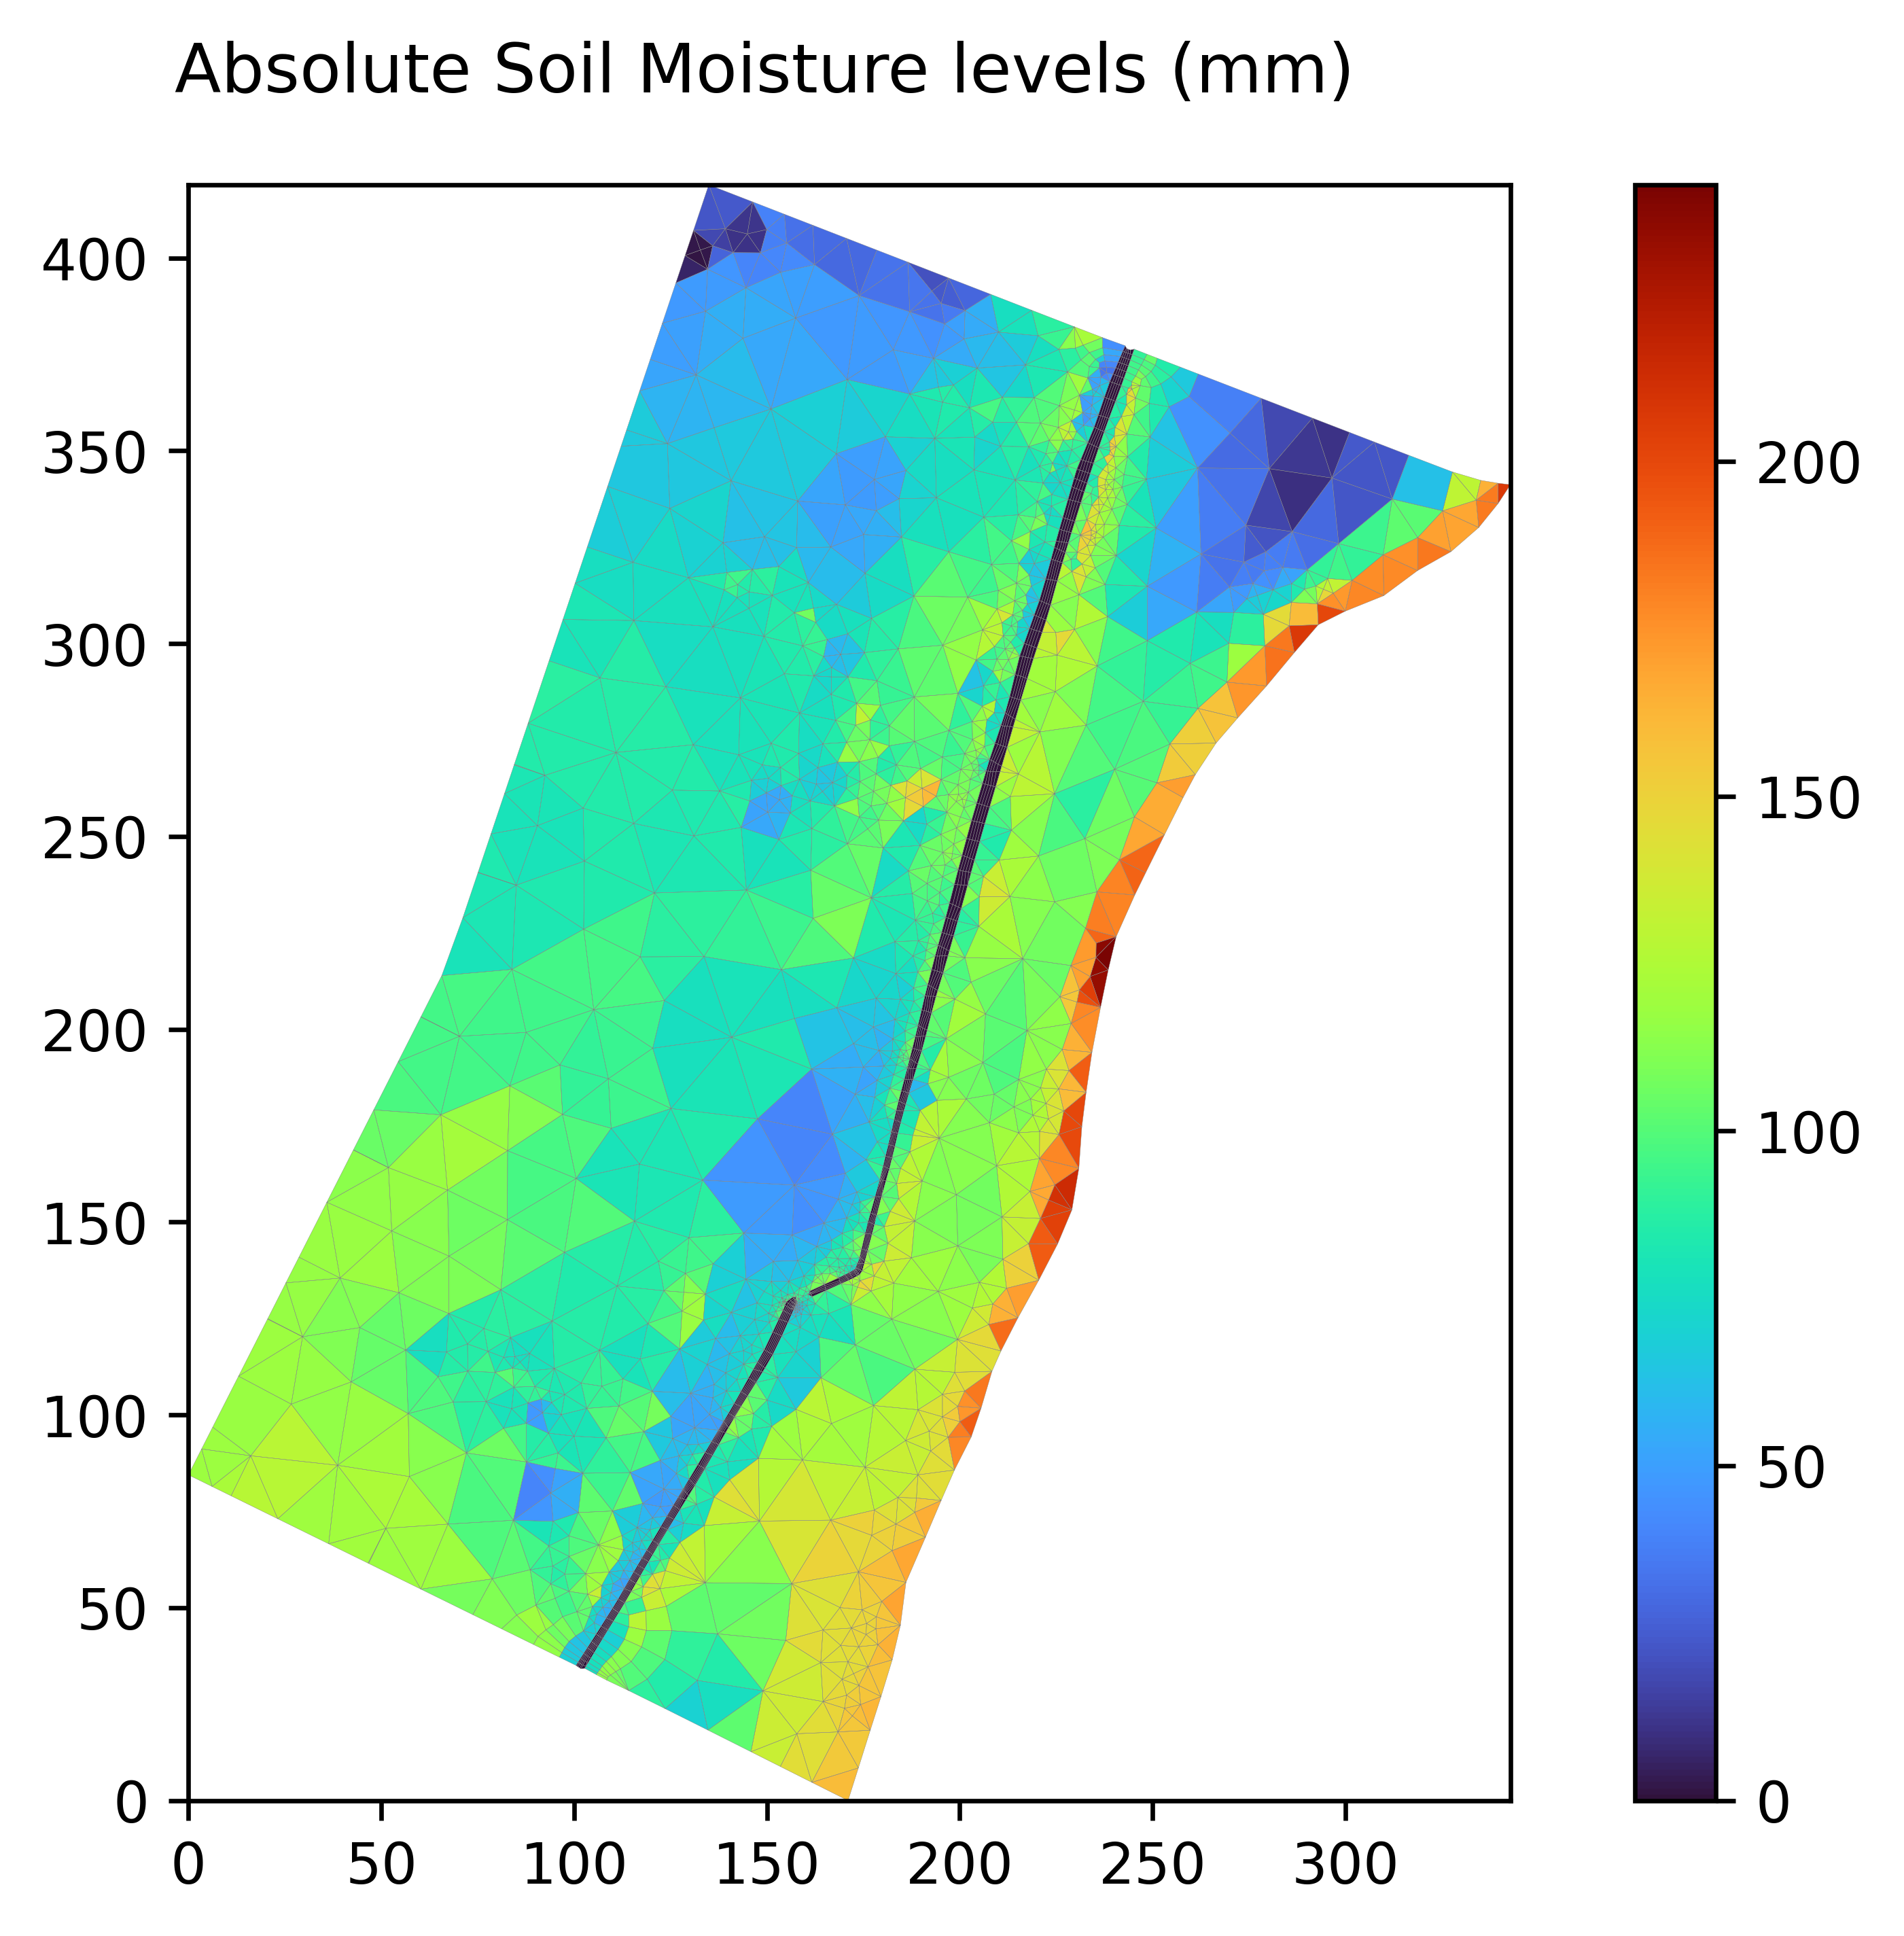
\includegraphics[width=0.9\linewidth]{PICTURES/models_res/sm_res}
\endminipage\hfill
\minipage{0.5\textwidth}
  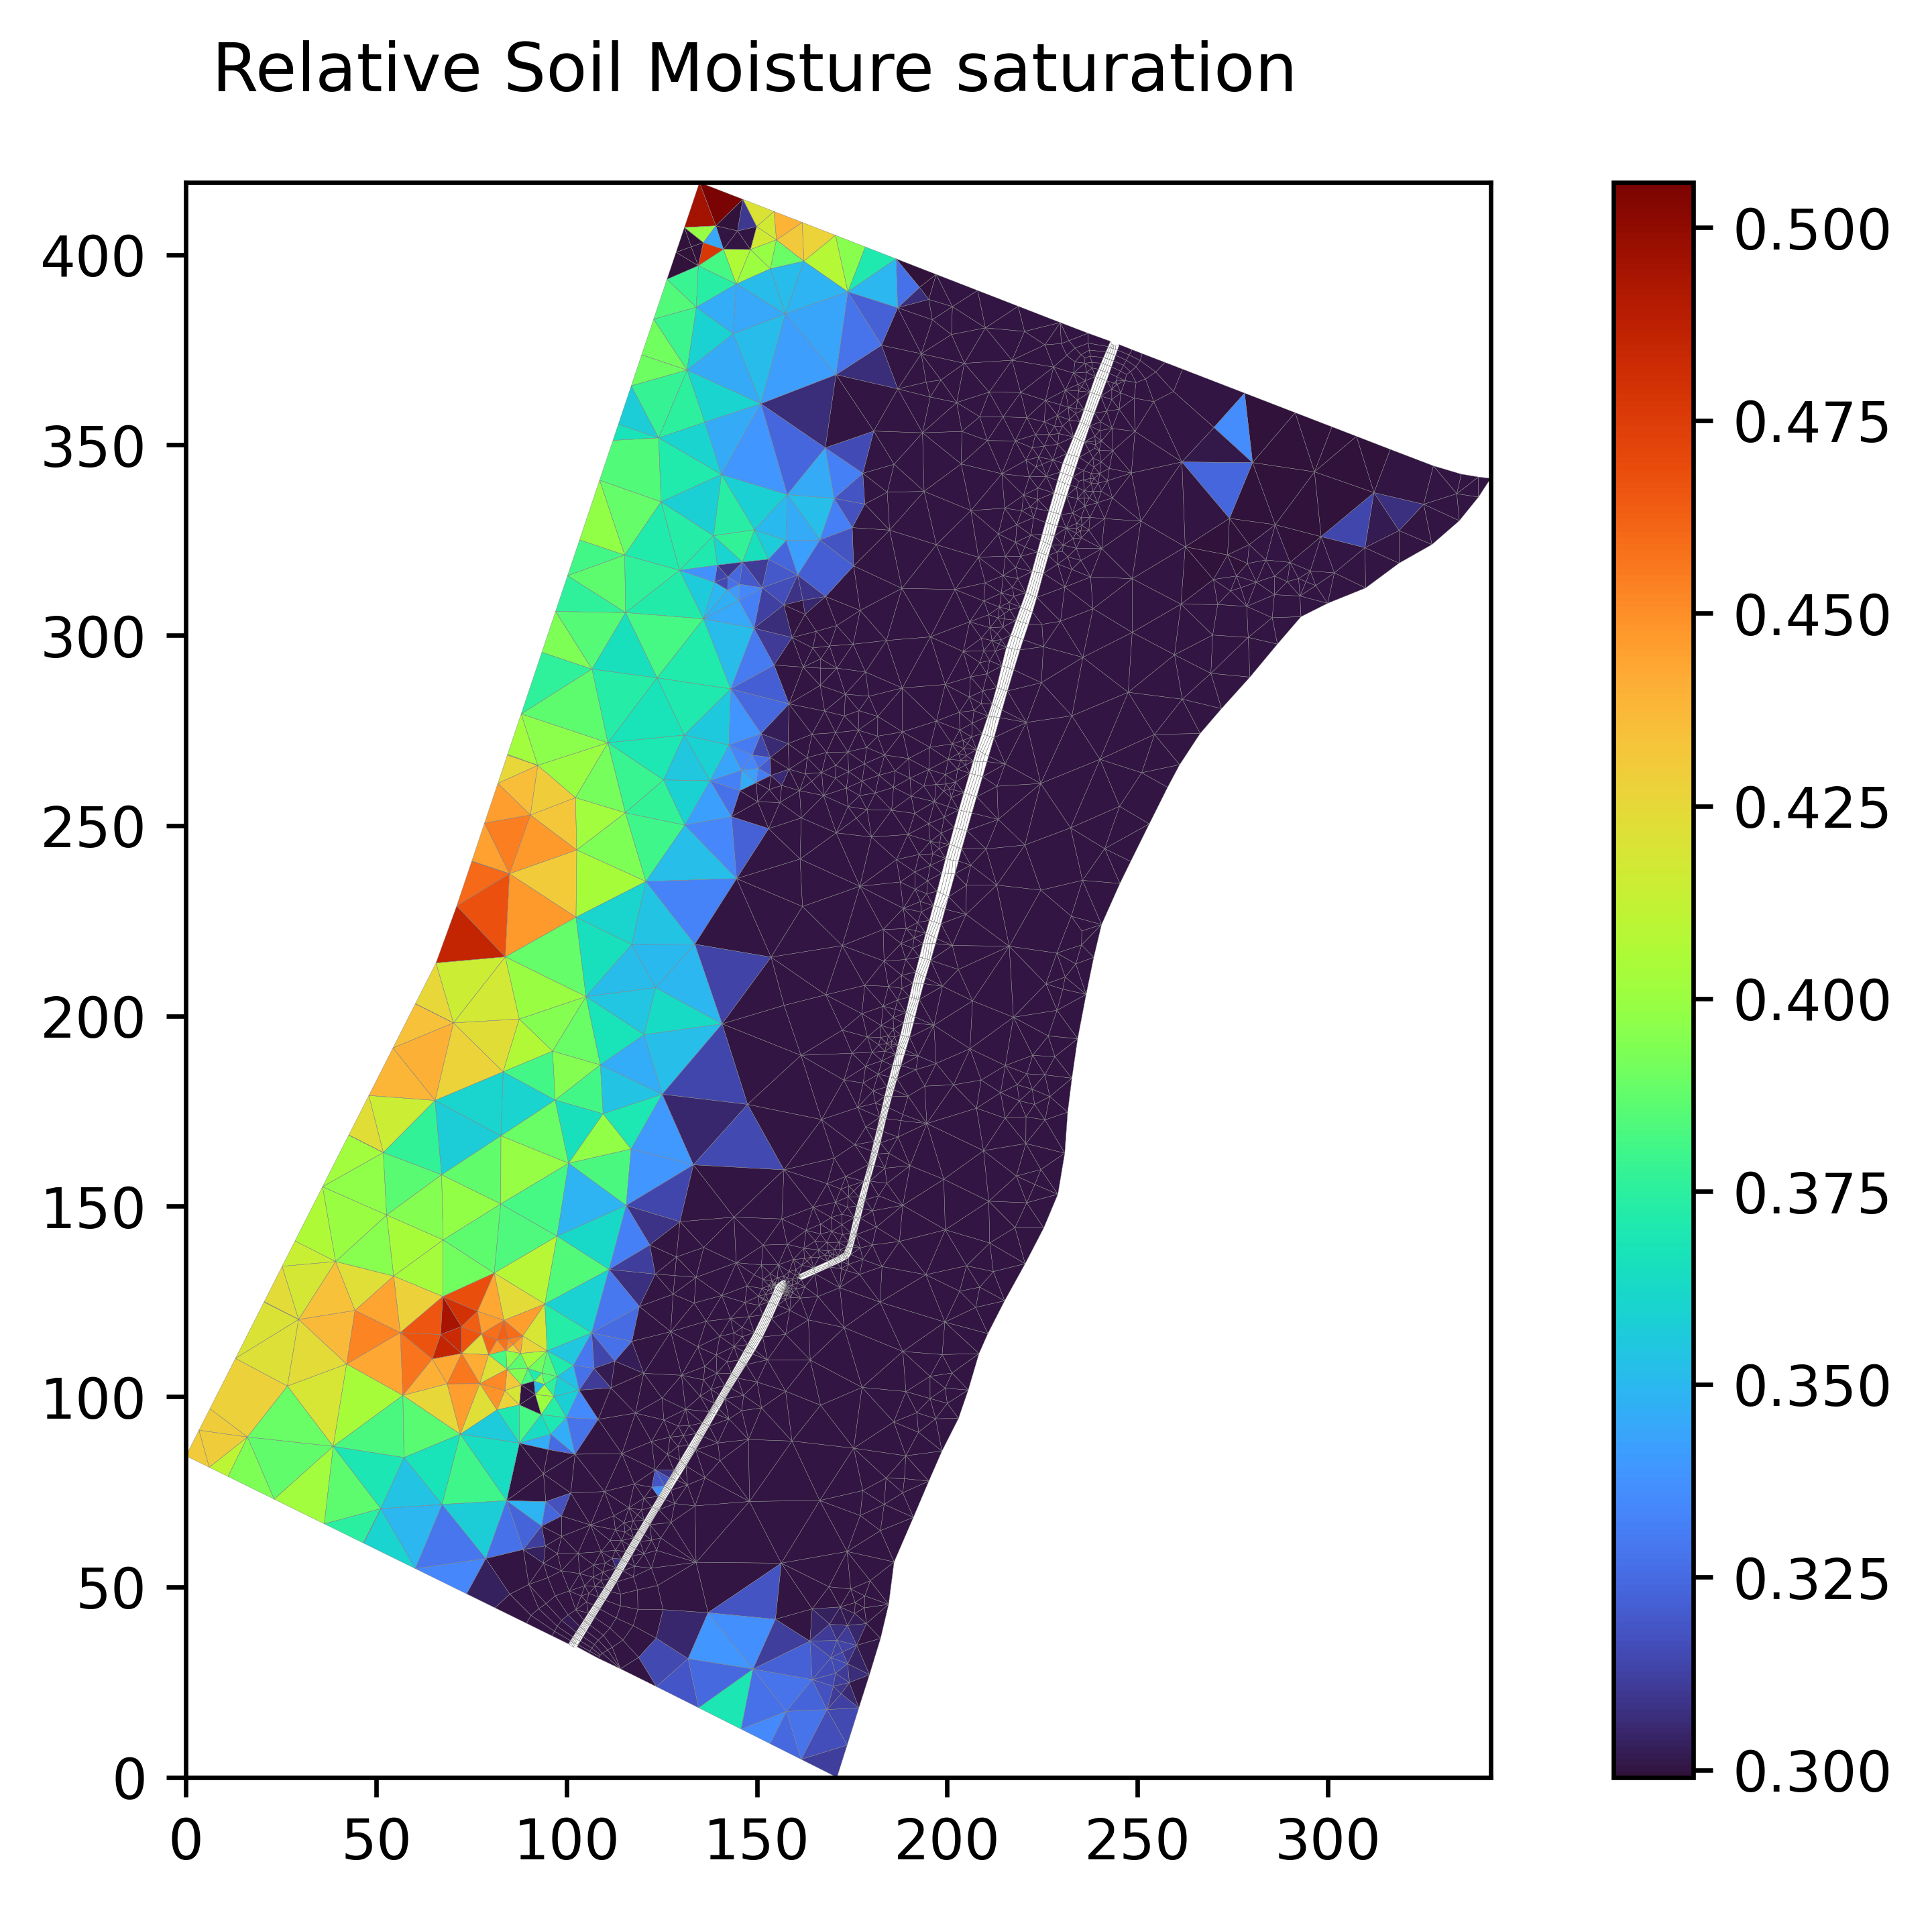
\includegraphics[width=0.9\linewidth]{PICTURES/models_res/sm_res_ratio}
\endminipage\hfill
\caption{Soil Moisture: left - absolute levels (mm); right - relative saturation.}\label{fig:sm_res}
\end{figure}

\begin{figure}[H]
    \centering
    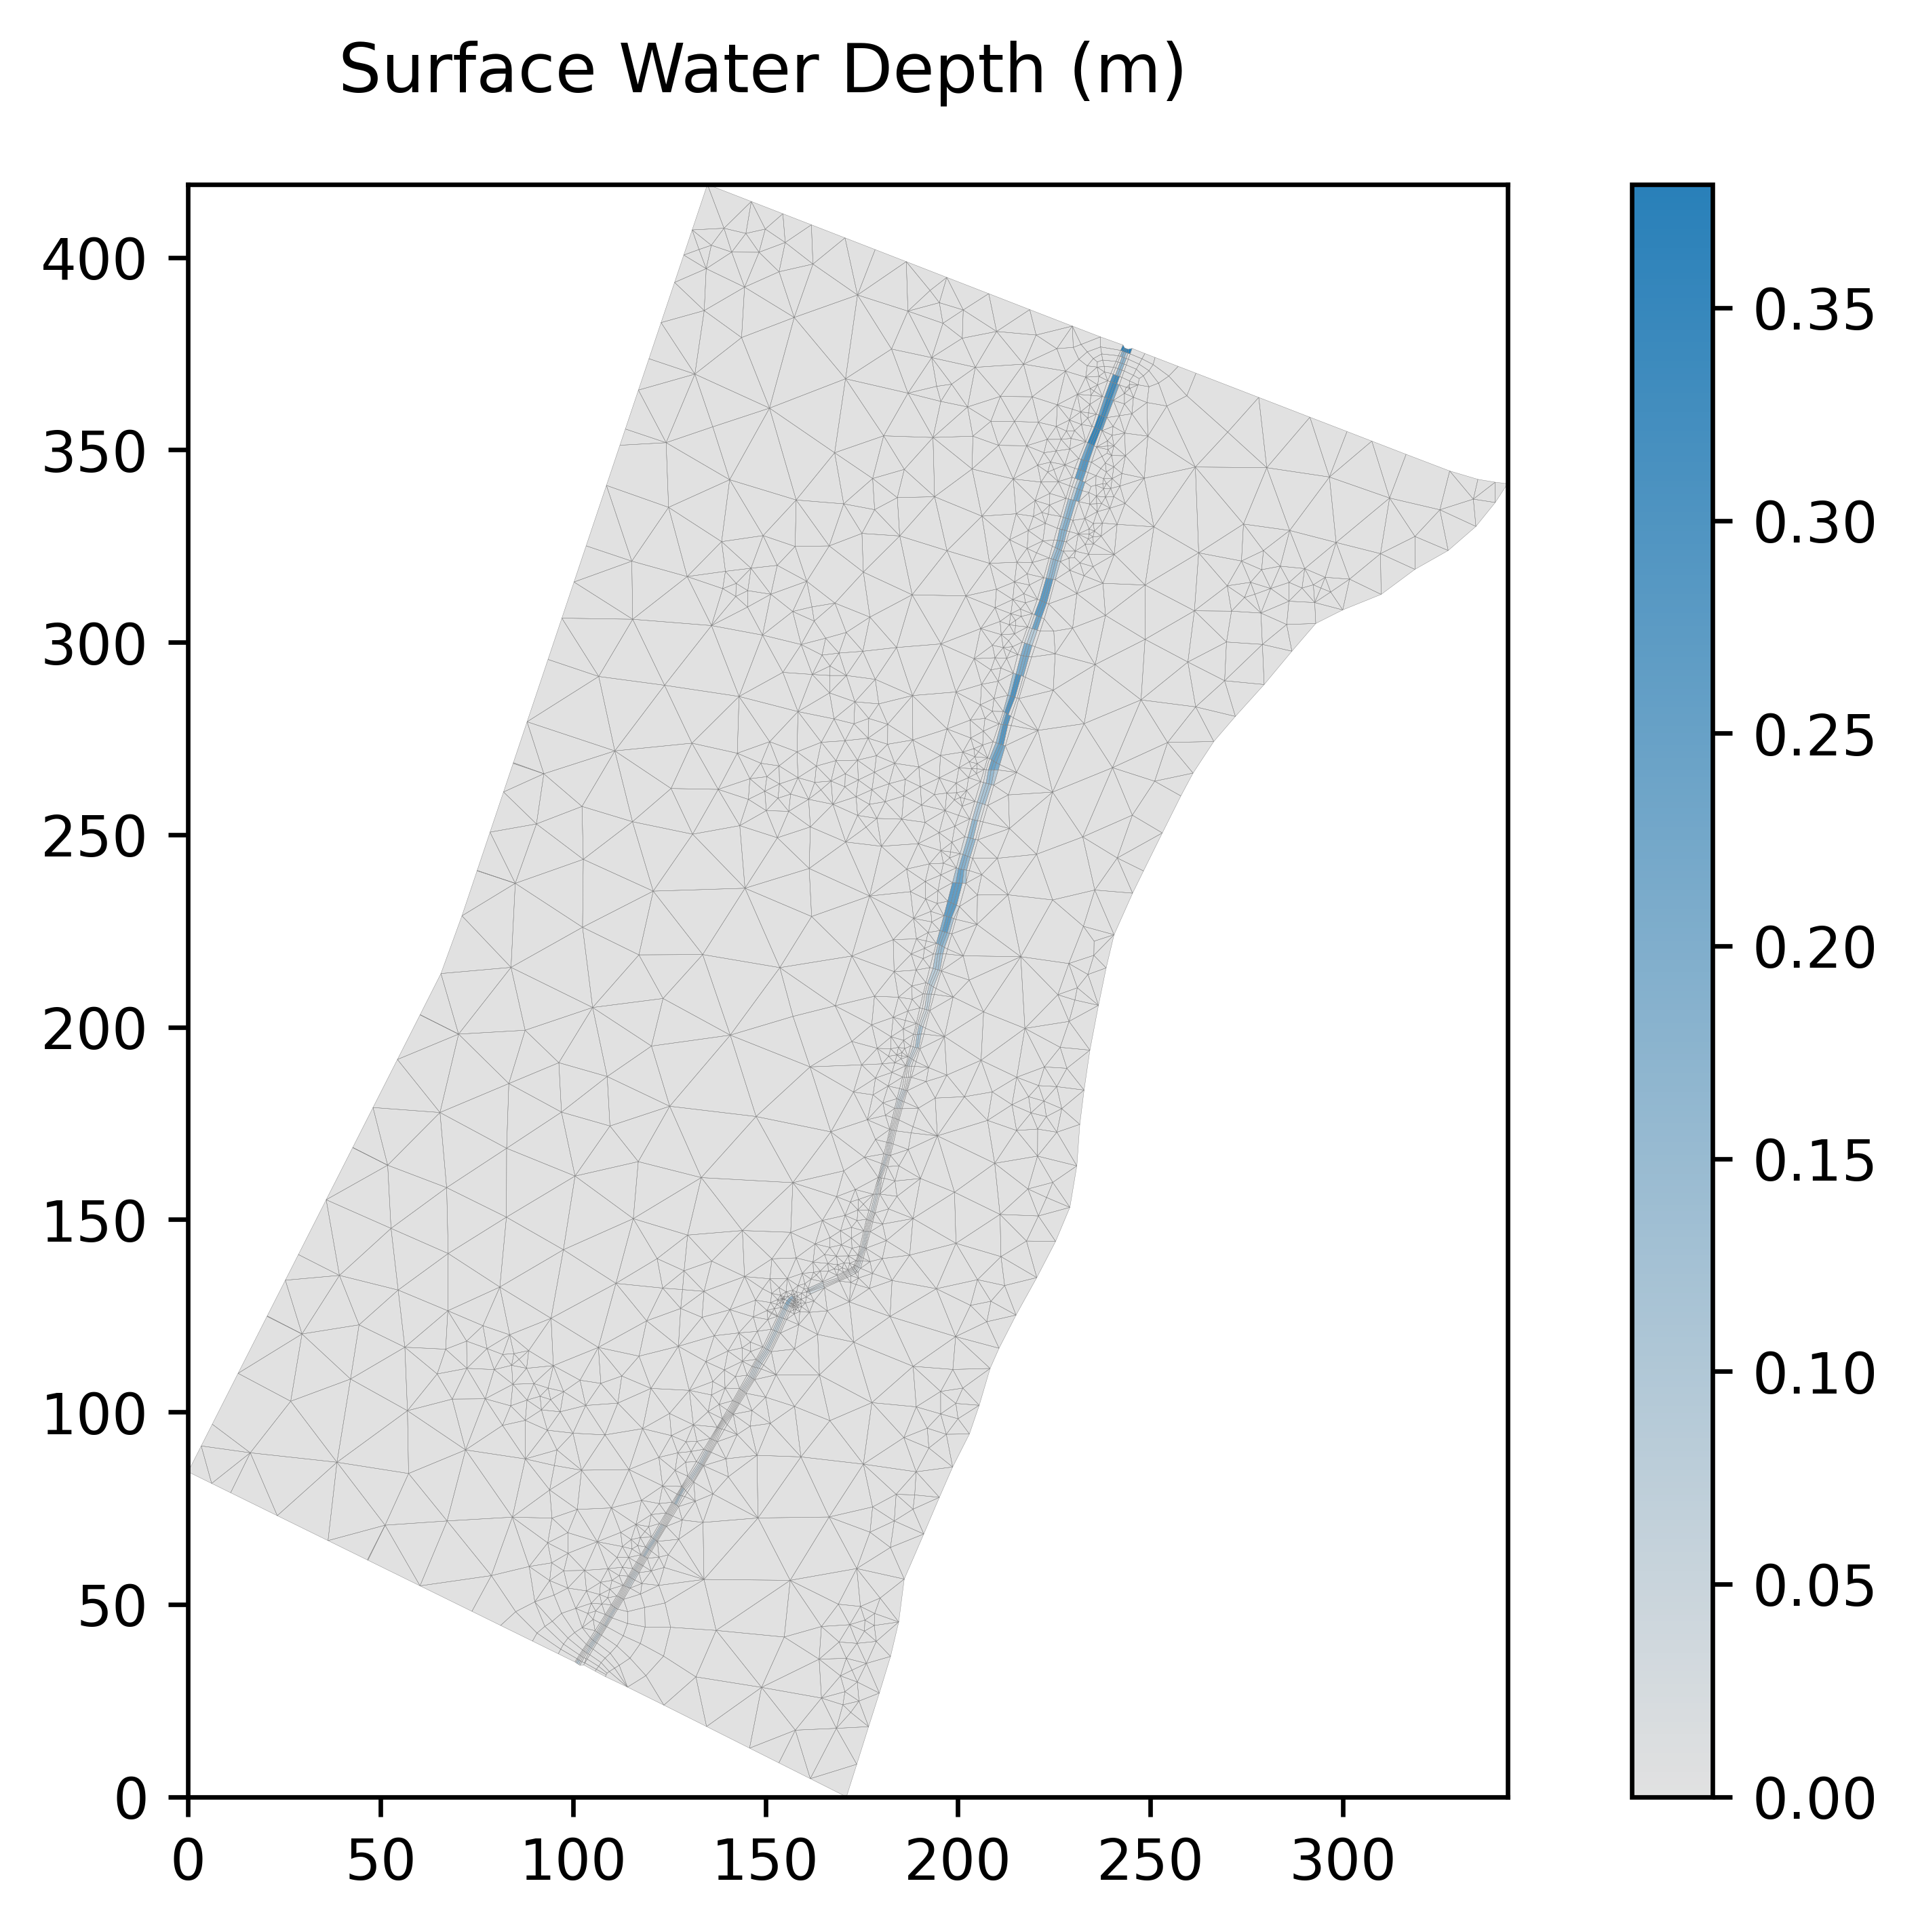
\includegraphics[scale=0.5]{PICTURES/models_res/sws}
    \caption{SW levels at the end of the simulation period.}
    \label{fig:sw_res}
\end{figure}



\section{Comparison with Measured Observations}
\label{obs}
The following plots compare the simulated and observed hydraulic heads at the observation locations as illustrated in \ref{fig:obs_pts}. It is observed that the simulated observations agree with the measured observations qualitatively in most locations. 

\begin{figure}[H]
    \centering
    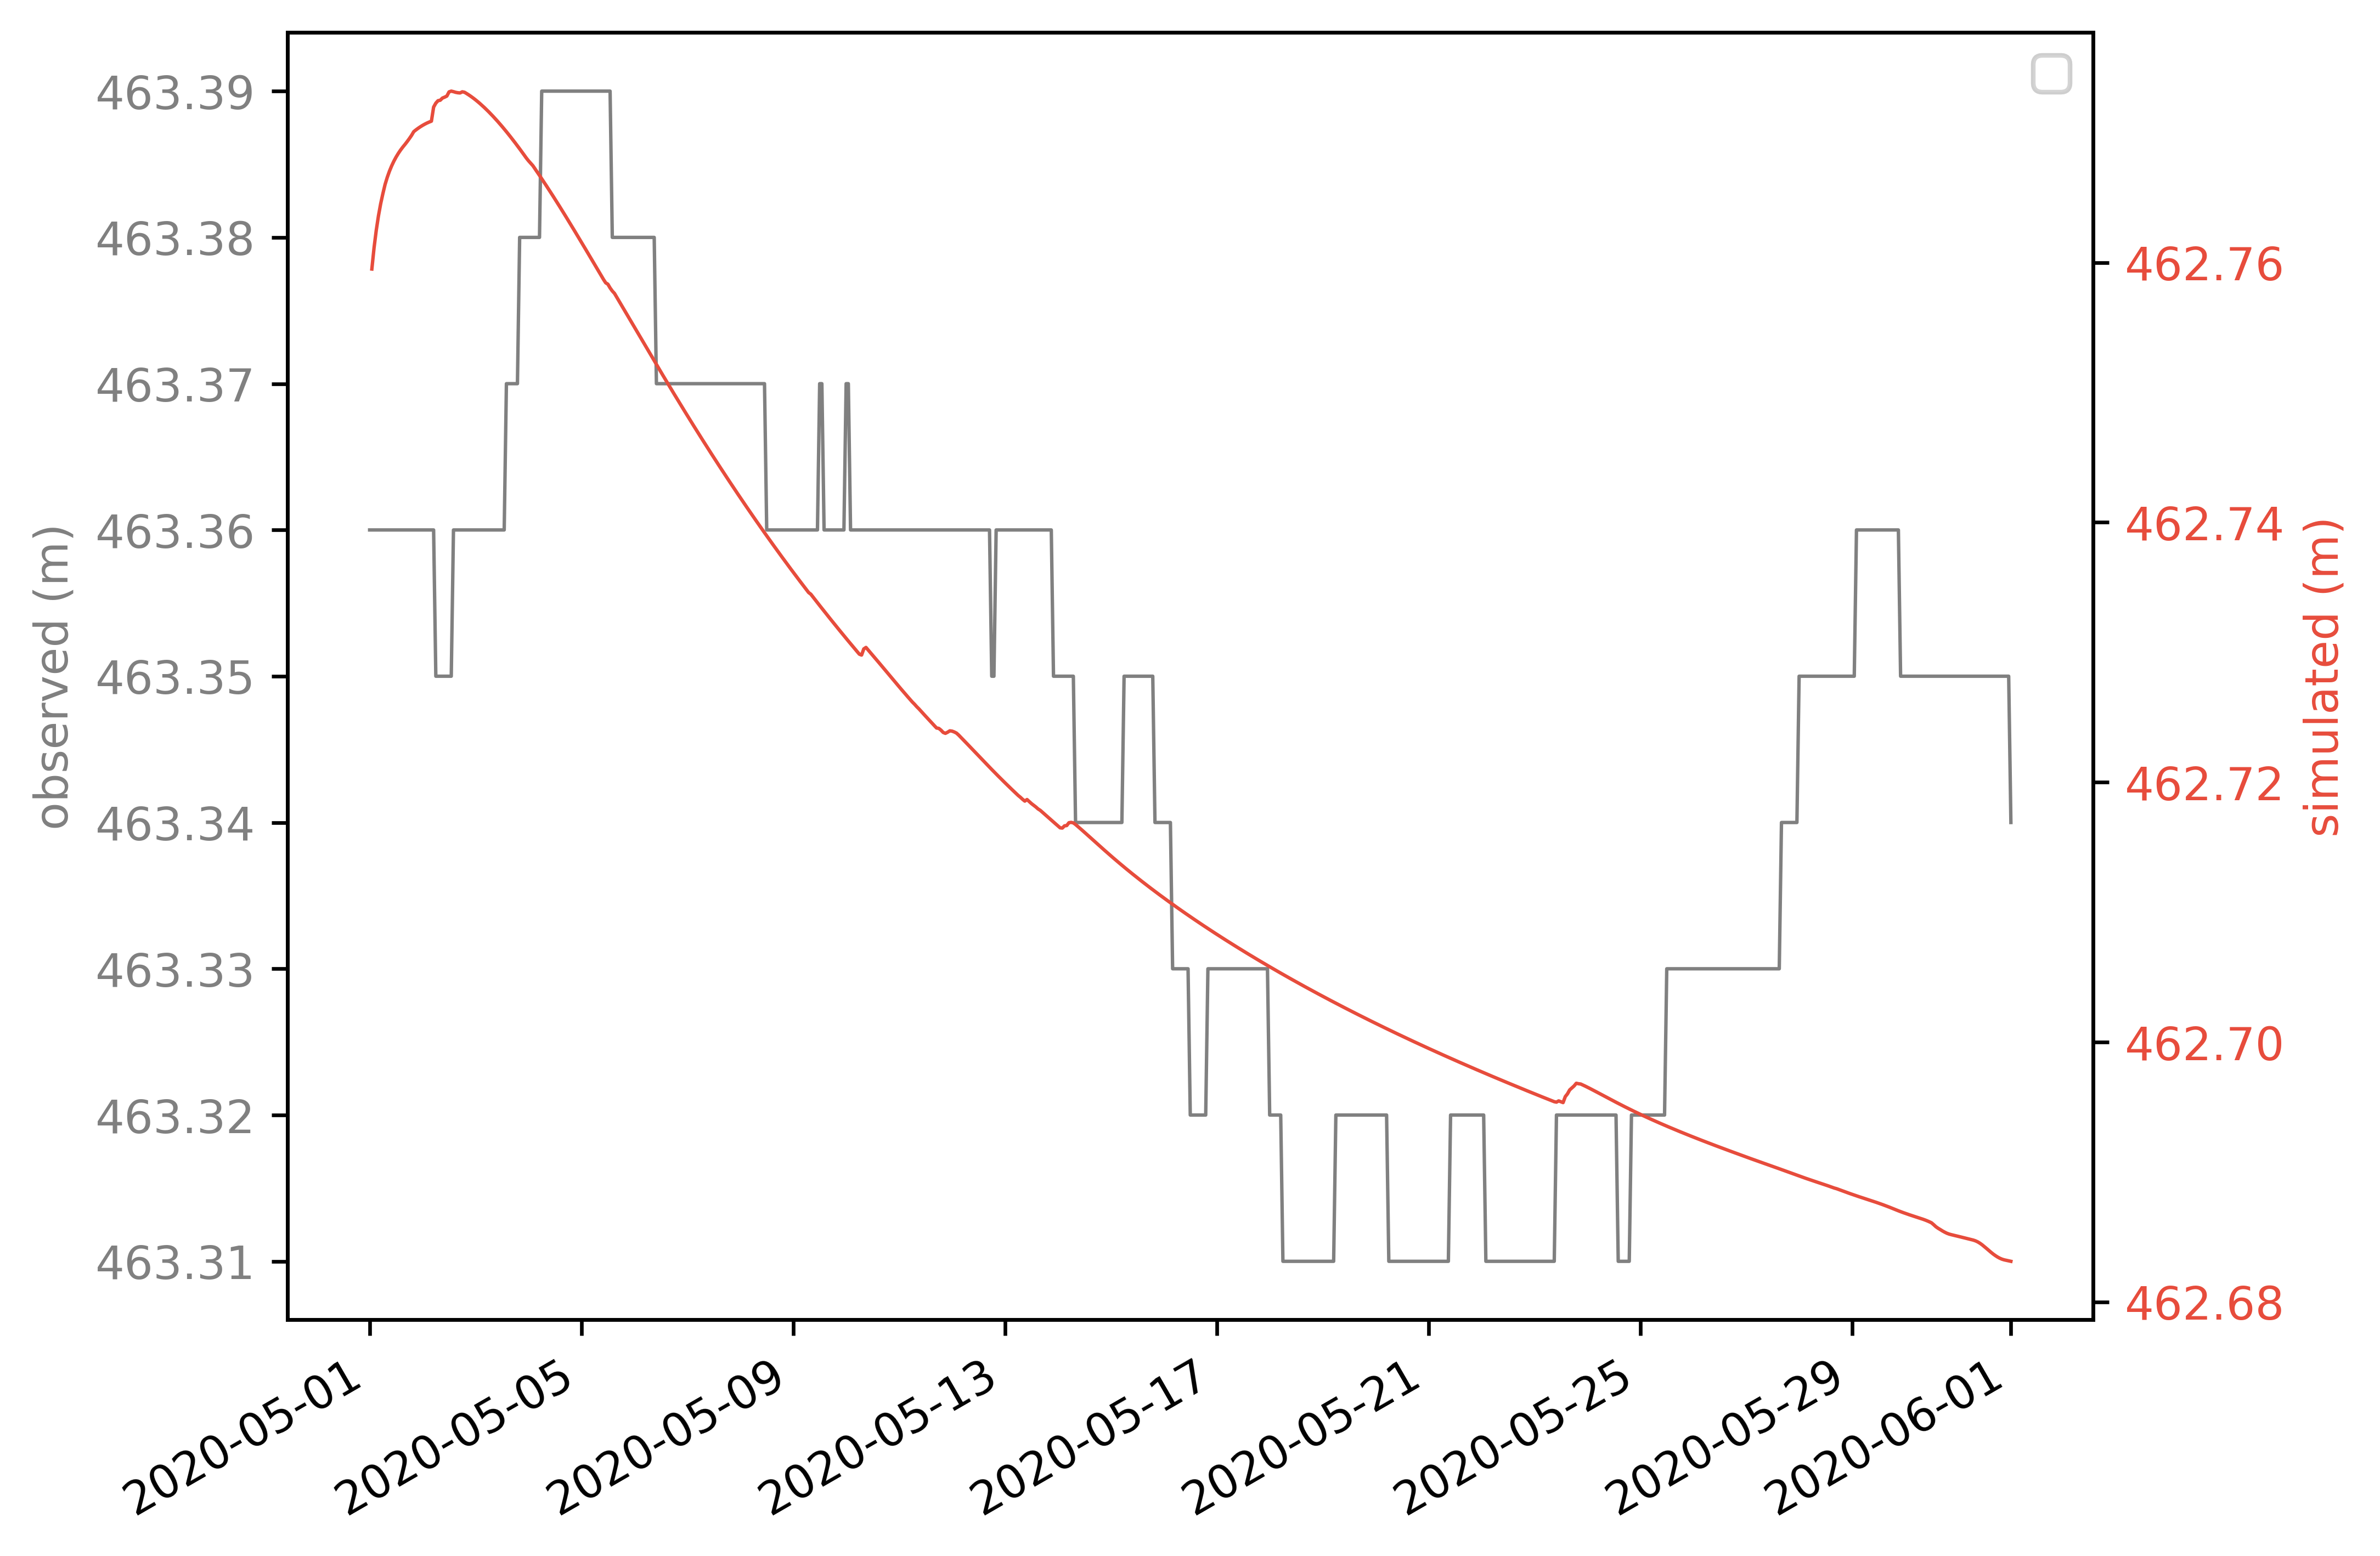
\includegraphics[width=\linewidth]{PICTURES/models_res/p2}
    \caption{Comparing simulated and measured observations at location P-2.}
    \label{fig:p2}
\end{figure}

\begin{figure}[H]
    \centering
    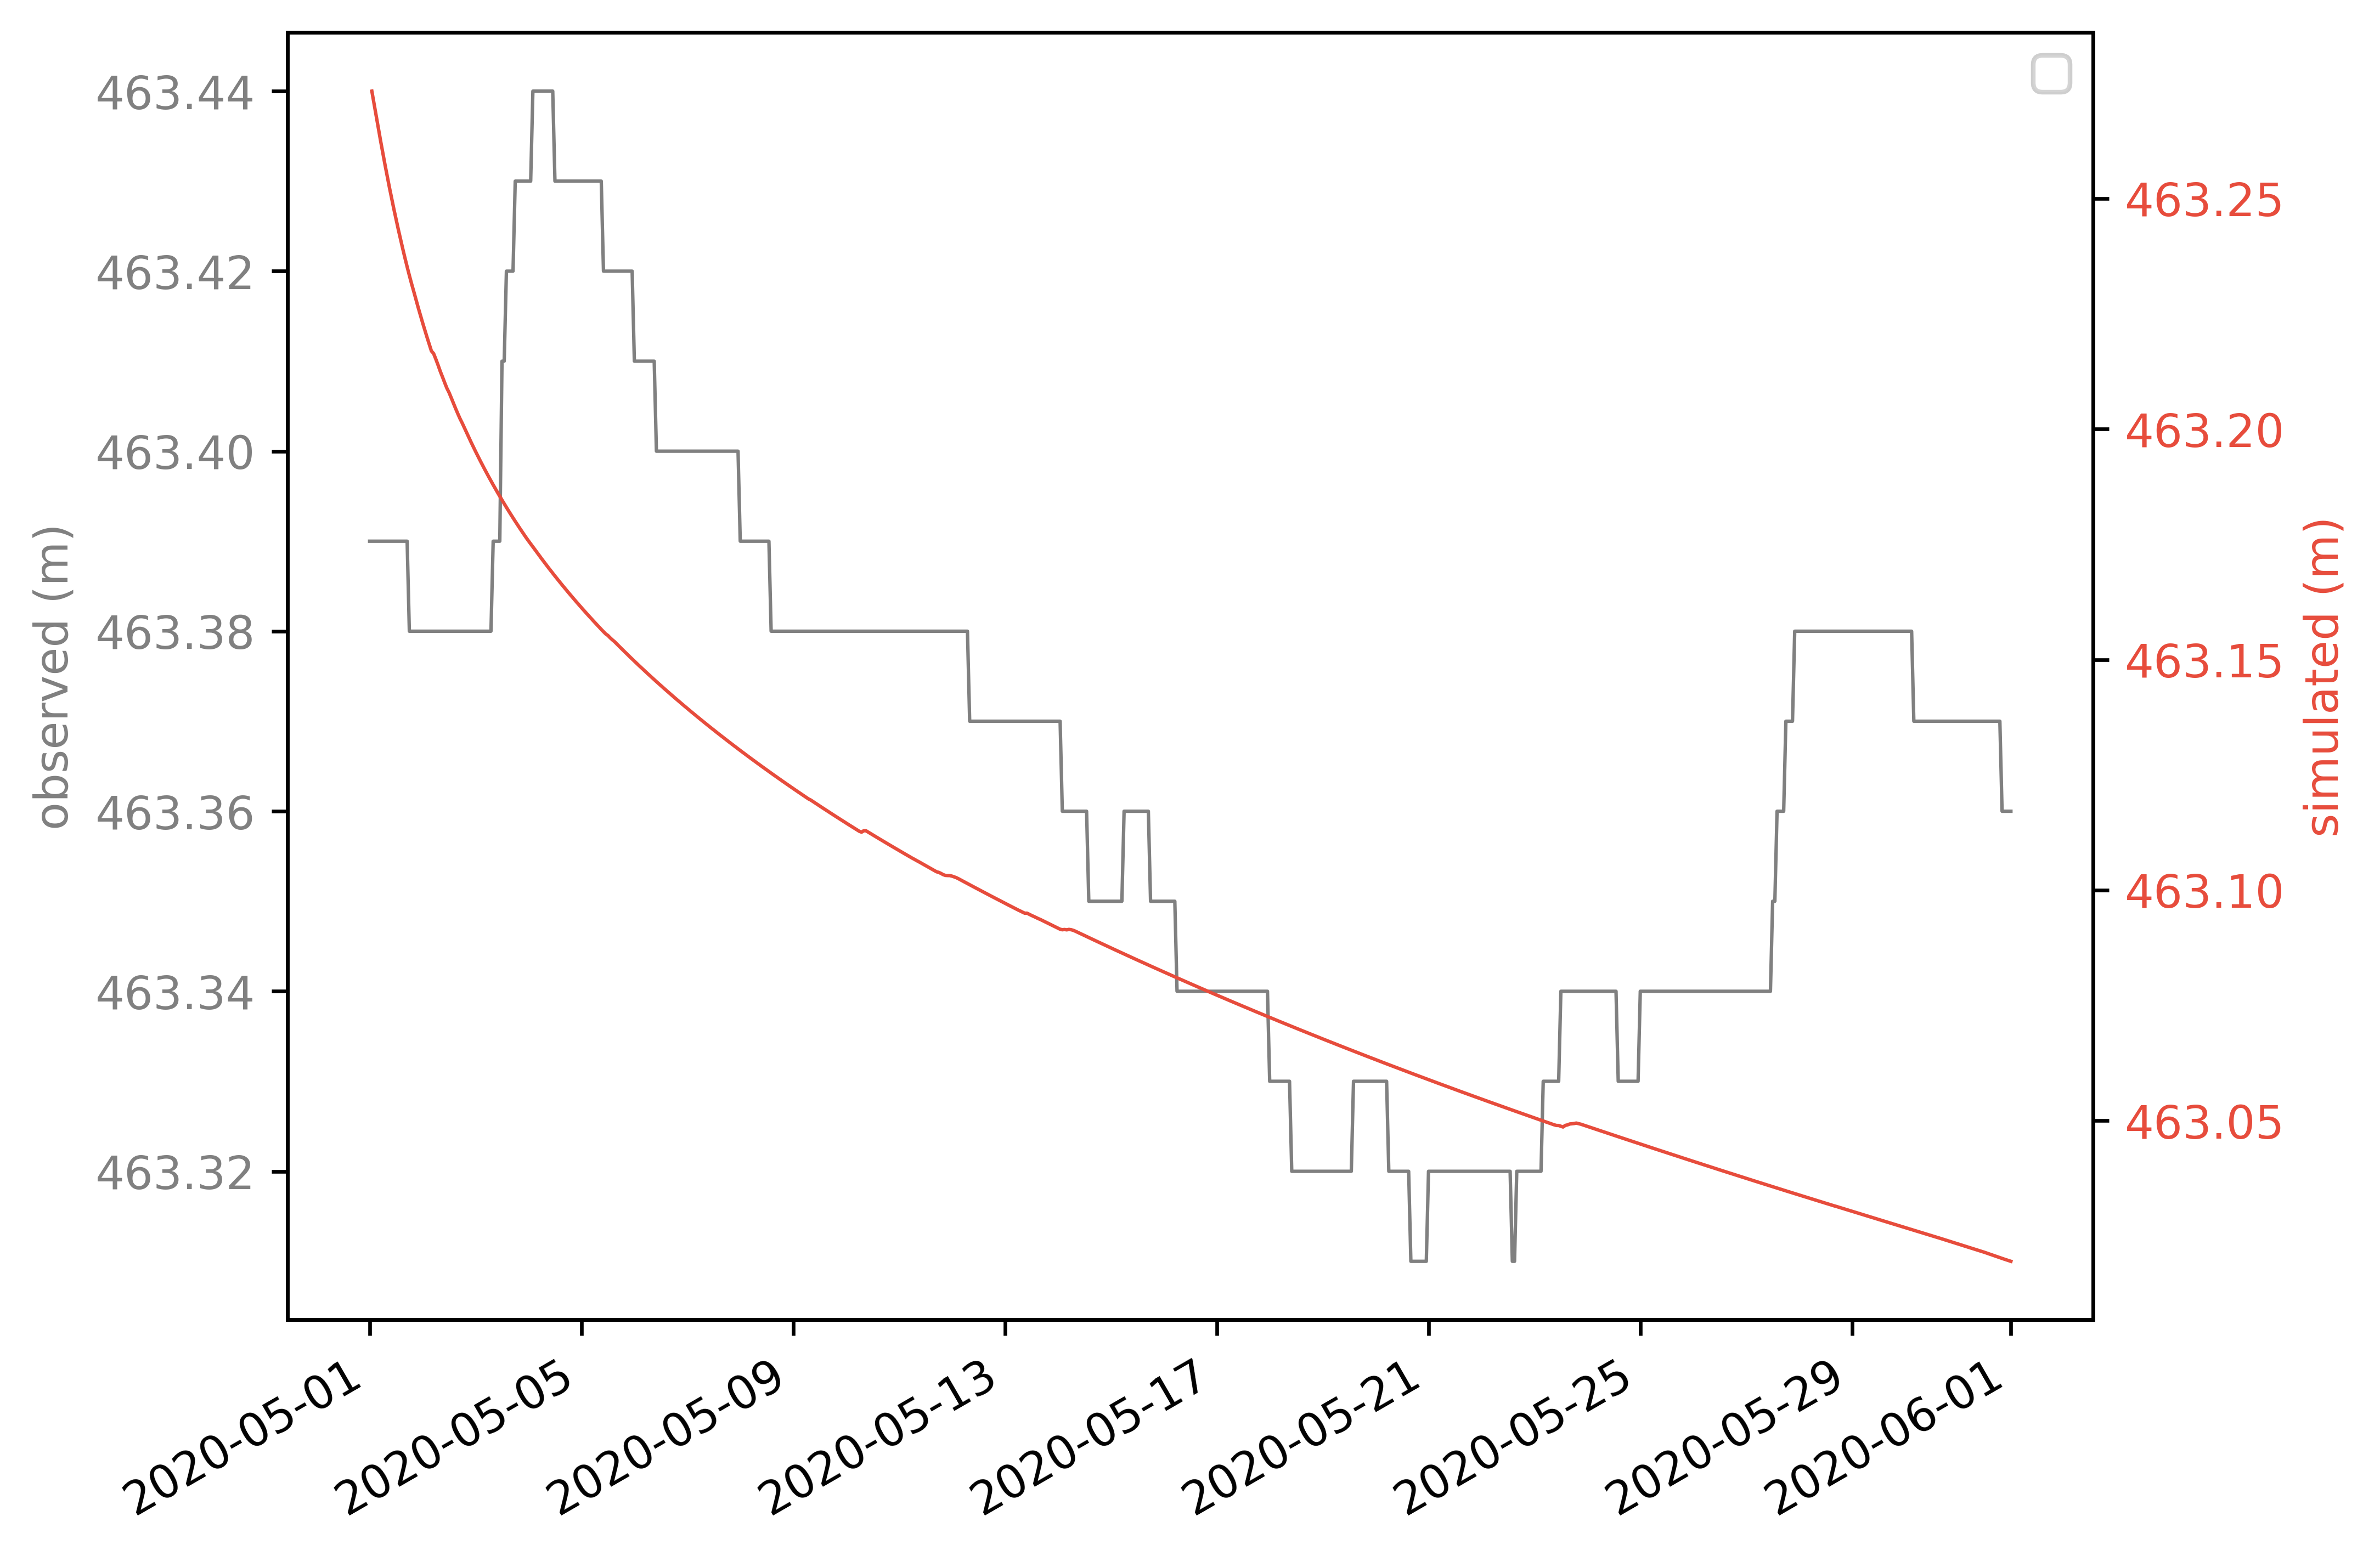
\includegraphics[height=0.42\textheight]{PICTURES/models_res/p1}
    \caption{Comparing simulated and measured observations at location P-1.}
    \label{fig:p1}
\end{figure}

\begin{figure}[H]
    \centering
    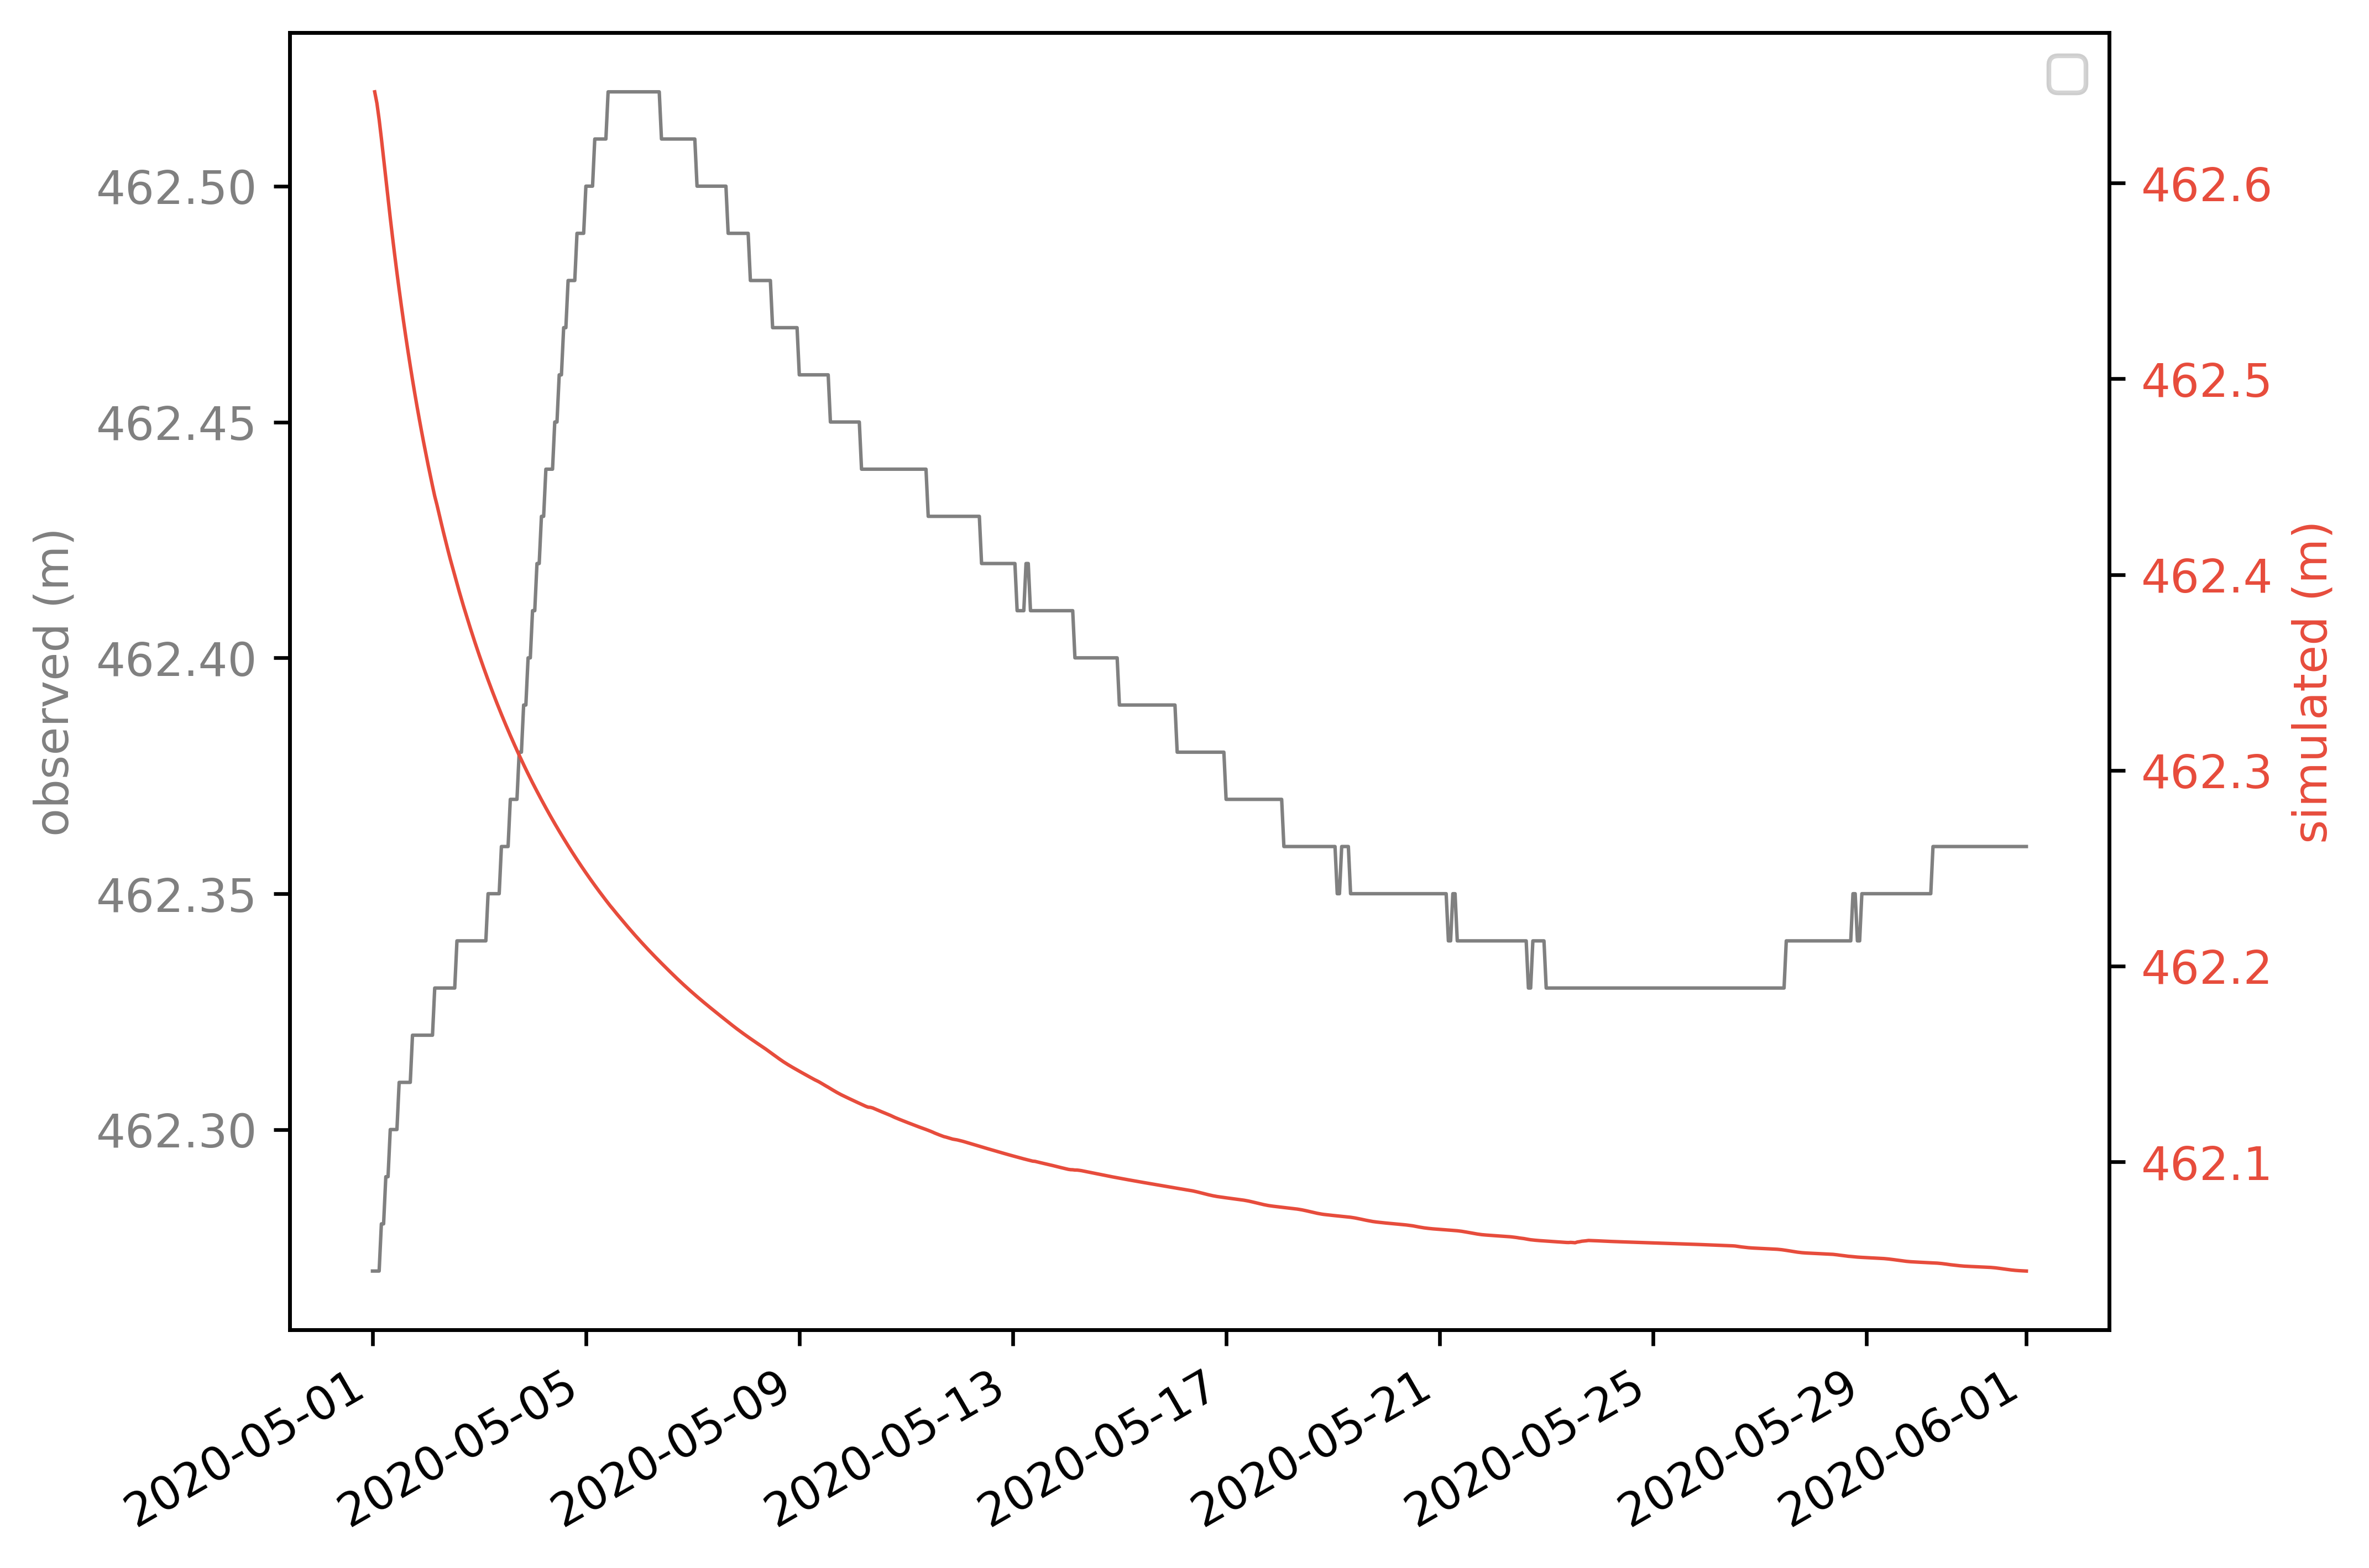
\includegraphics[height=0.42\textheight]{PICTURES/models_res/p12}
    \caption{Comparing simulated and measured observations at location P-12.}
    \label{fig:p12}
\end{figure}

\begin{figure}[H]
    \centering
    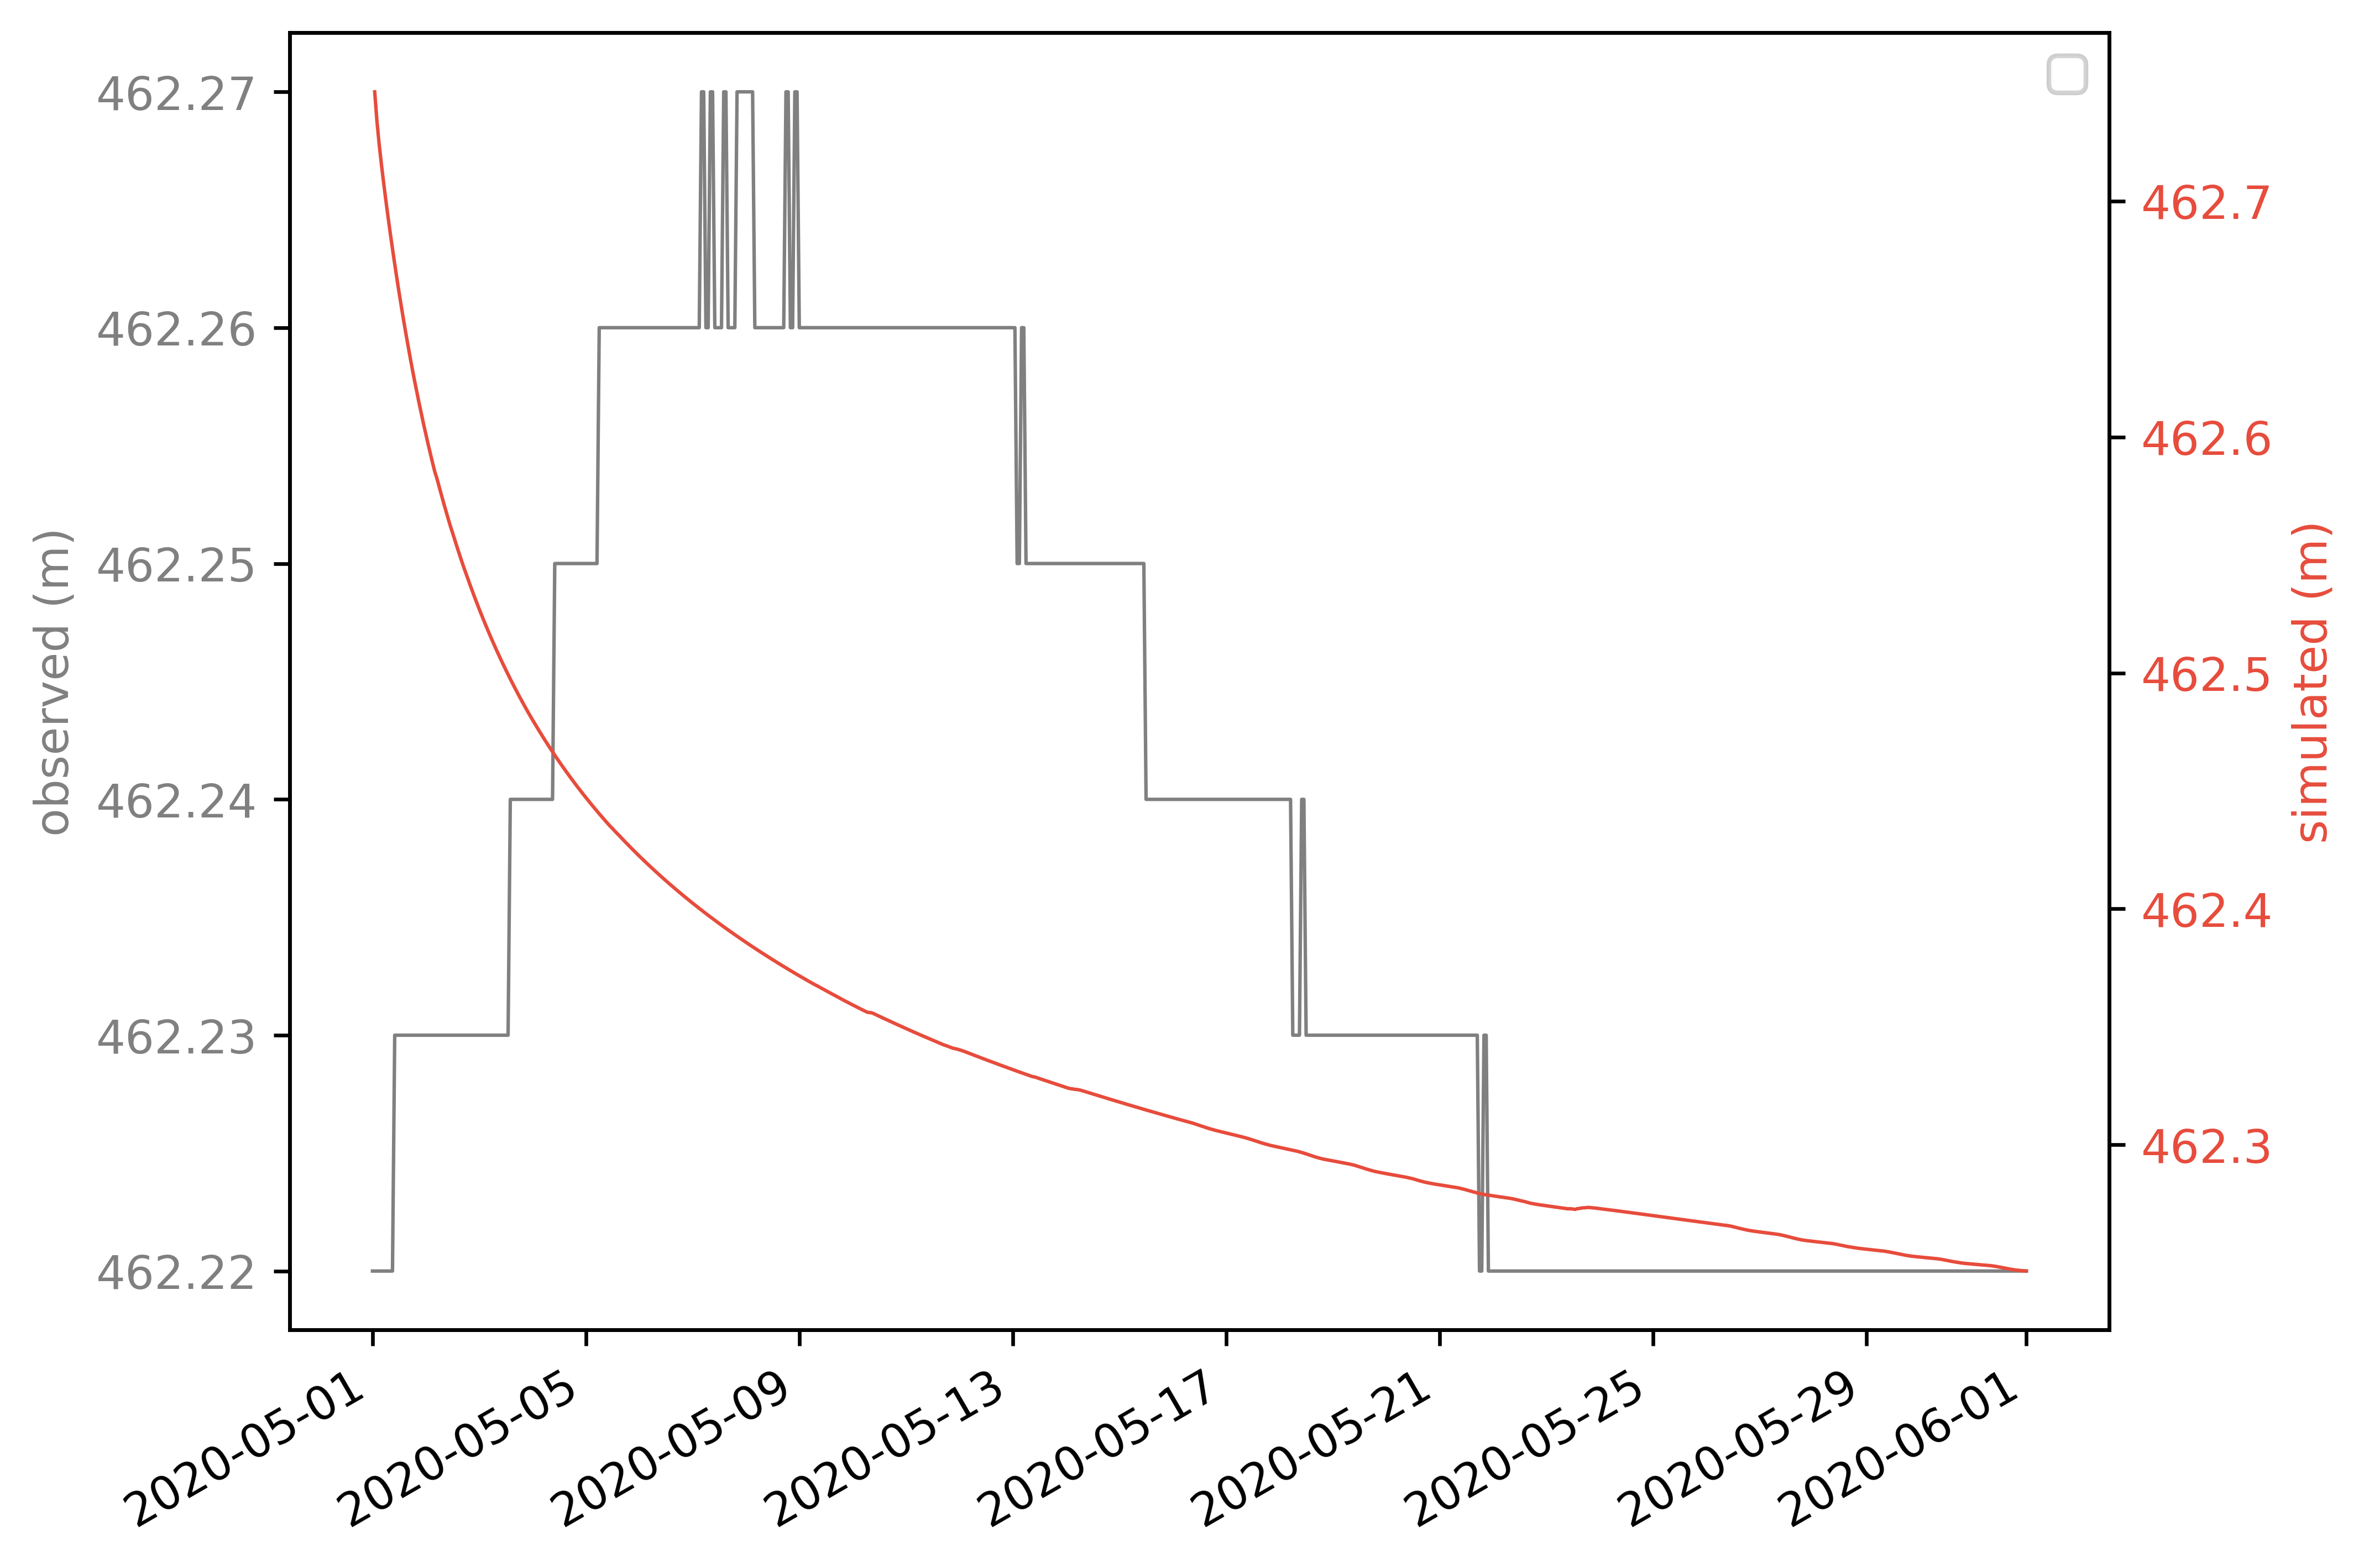
\includegraphics[height=0.42\textheight]{PICTURES/models_res/p6}
    \caption{Comparing simulated and measured observations at location P-6.}
    \label{fig:p6}
\end{figure}

\begin{figure}[H]
    \centering
    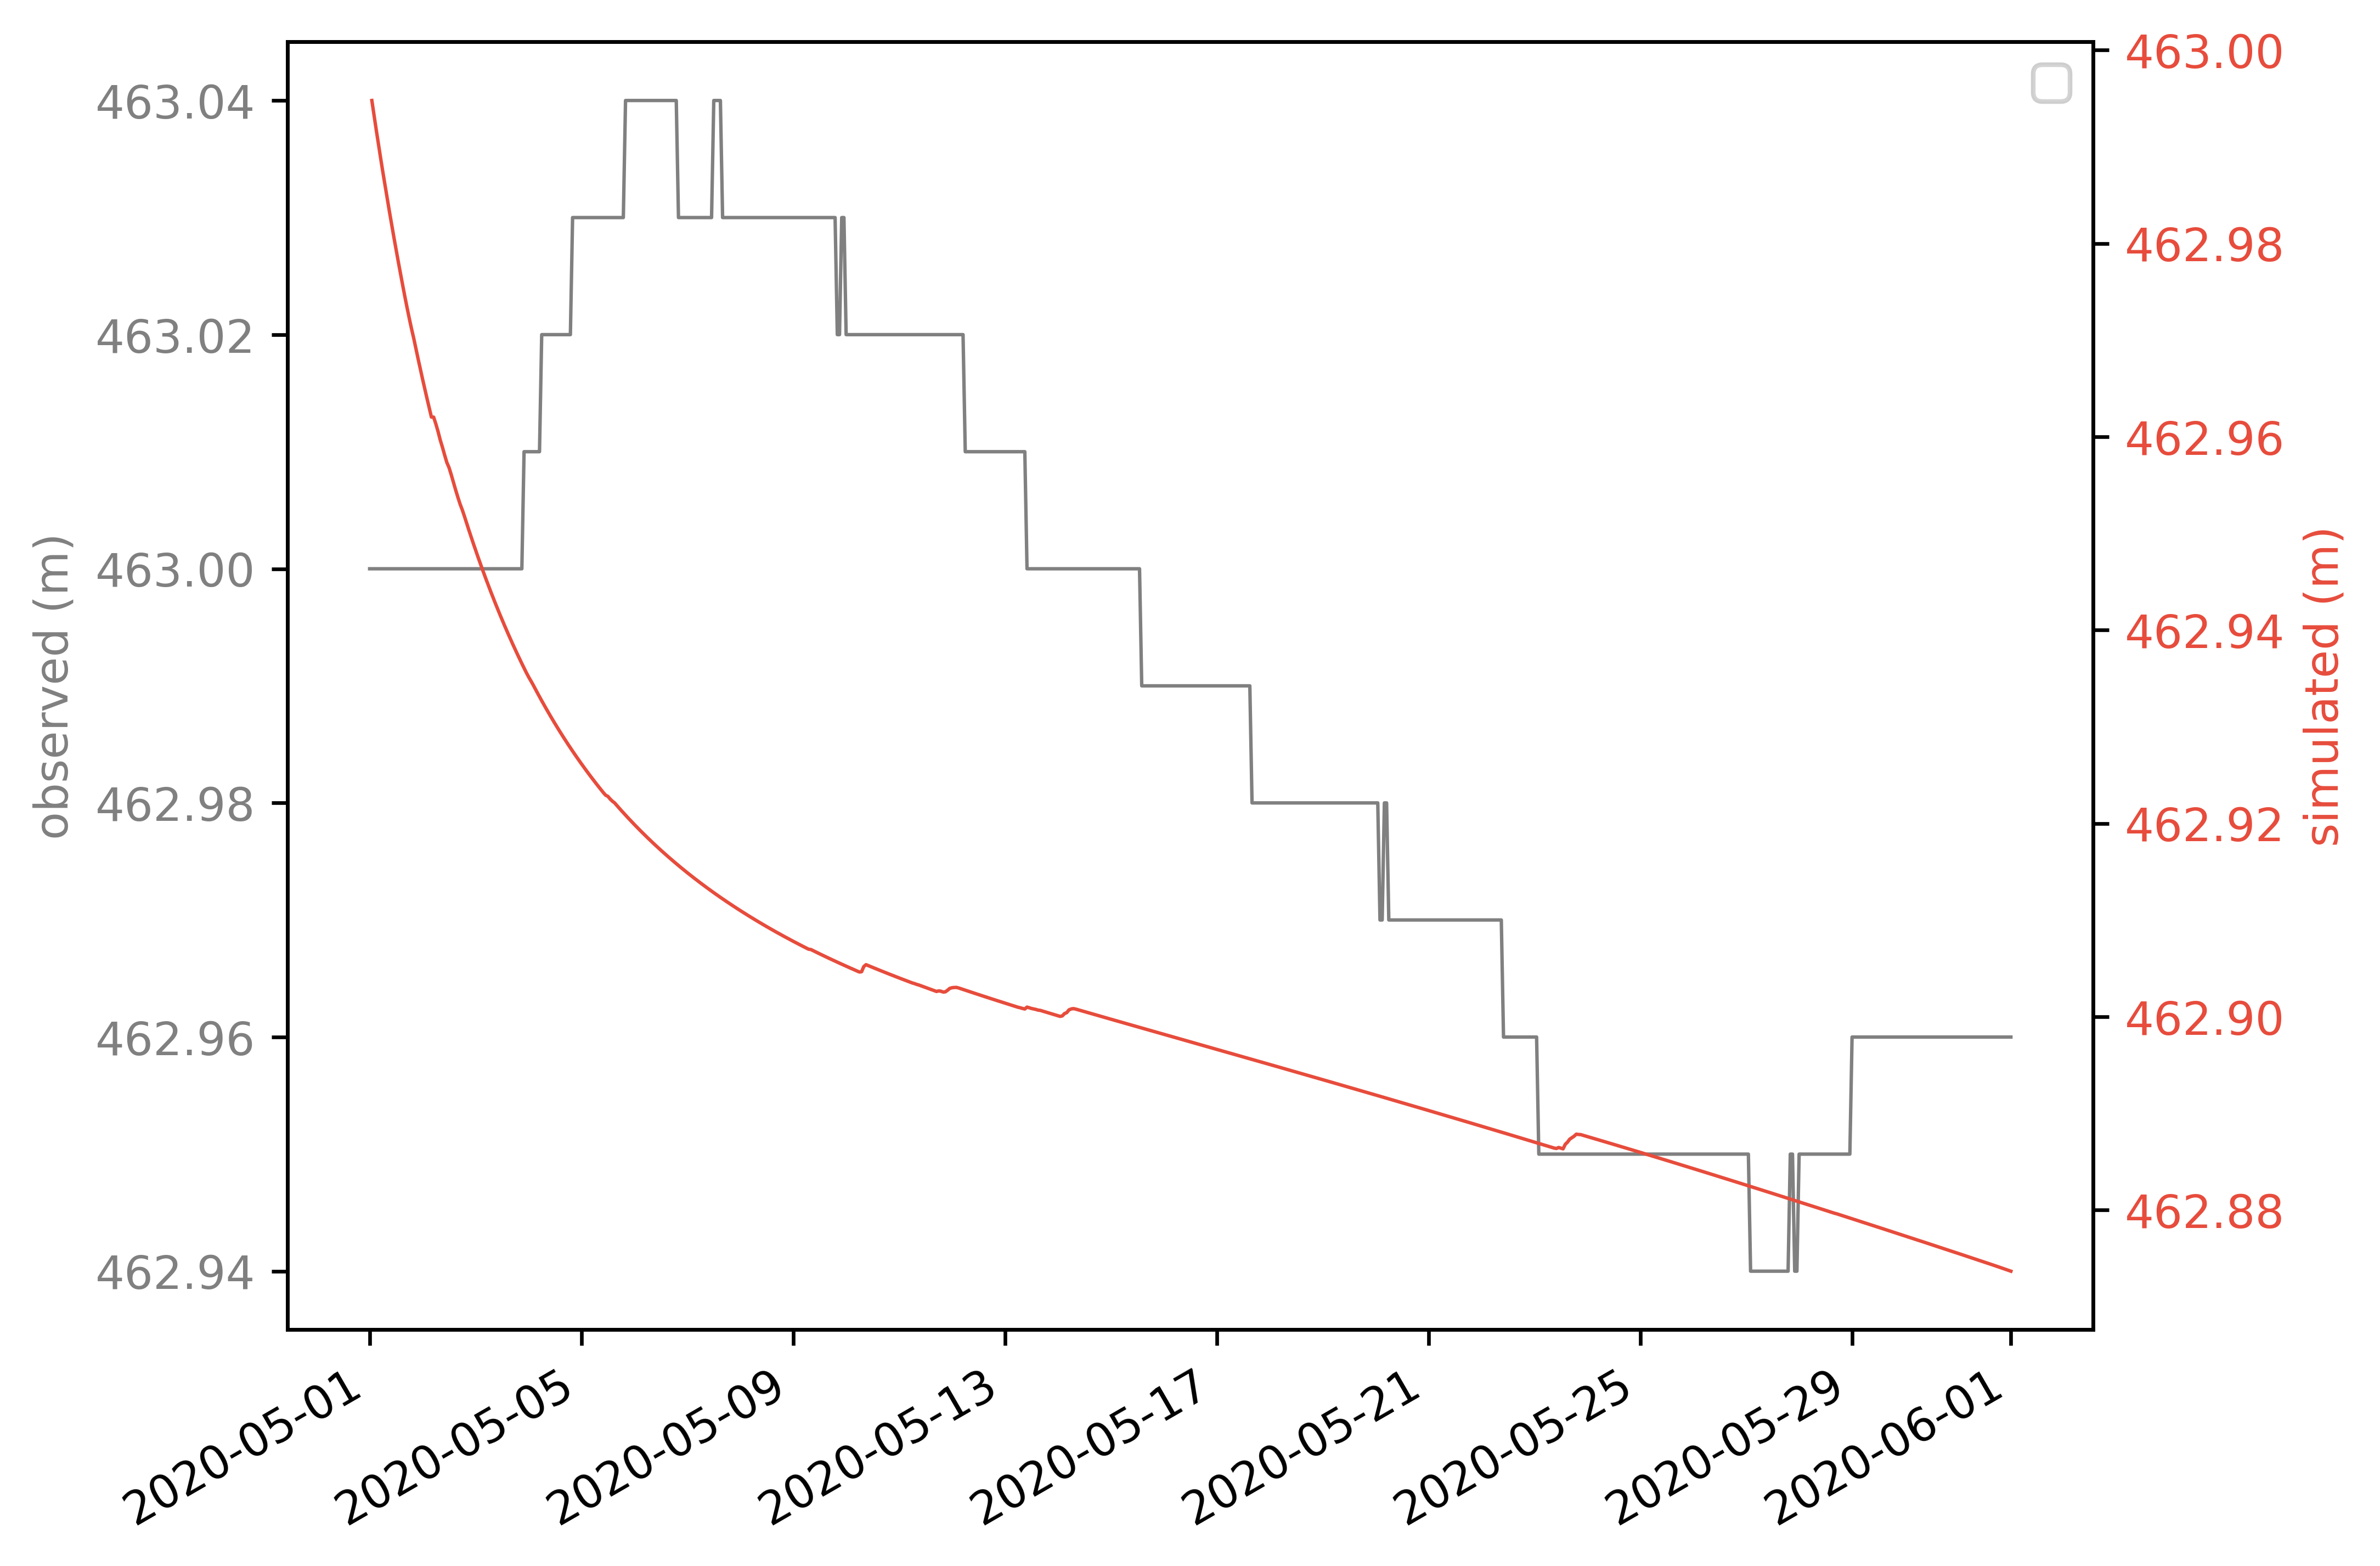
\includegraphics[height=0.42\textheight]{PICTURES/models_res/p7}
    \caption{Comparing simulated and measured observations at location P-7.}
    \label{fig:p7}
\end{figure}

\subsection{Addressing the Discrepancy}
One must note that the simulation set up was rather bare and is lacking in depth of representing the reality numerically. No calibration of either of the three models has been carried out. As discussed previously, GWSWEX model, being a conceptual model, demands extensive calibration. Furthermore, the initial conditions are very rough approximations that seem to be inadequately representative of the conditions observed in the study area. In this light, the simulated observations look rather quite promising.
\\ \\
The simulation may be improve with:
\begin{enumerate}
    \item calibration of GWSWEX, GW, and SW models,
    \item a better description of the GW model - especially the thickness of the unconfined zone,
    \item either improving the initial conditions to adequately represent the observed conditions in the study area, or running the simulation for a longer period of time and discarding the initial results to a point from where the measured and simulated observations agree quantitatively, adequately.
    \item improving the quality of P and ET inputs, and
    \item a finer temporal and spatial descretisization. 
\end{enumerate}

In the above list of improvements, Point (2) is crucial to the quality of the model results as the GWSWEX model heavily relies on the geometry to calculate GW and SM fluxes. It is known that the GW model used in this study does not have an adequately realistic representation of the study area as in some areas, as in observation locations P-2, P-1, and P-6, the model top in the GW model does not correspond to the measured elevations at these locations.
\\ \\
The study area lies almost in the middle of three meteorological stations. Thus, by combining  precipitation data from all three stations instead of using the data from just one (as is the case in this study) may further improve model results.
\\
Furthermore, the study enforced potential evapotranspiration directly. The model results might imitate the measured observations better if one enforced actual evapotranspiration instead.
\\ \\
The initial conditions are based purely on speculations from observing the measurements from the few observation locations that lie in the model domain. The relatively short simulation period of 1 month might not be adequate to allow the initial state of the model to achieve equilibrium. Thus, either a significantly longer simulation period and the assessment of the time scale at which the initial conditions no longer have an effect on the model results need to be determined for more reliable results.
\\ \\
For the sake of a testing and debugging, the simulation used coarse temporal and spatial descretisizations. The effects of varying temporal resolutions, which might be a crucial factor in explicit coupling schemes, are not studied. There is good scope for such a study.

\endinput